\documentclass[
 nopagenumber, exercisesheet, %% L'un
 answers,                     %% Ou l'autre 
 %noexercisenumber,
]
{kholles}


\title{Le fascicule de khôlles}
\author{Guillaume Bermudez, Baptiste Corrège}
\date{}
\mail{guillaume.bermudez@ens.fr, \qquad baptiste.correge@ens.fr}

% \title{}
% \author{}
% \mail{}

%Refs
\bibresource{misc/sources}

% \usepackage{pdfpages}
% \usepackage{circuitikz}

%%%%% EXERCICES %%%%%
\begin{document}

\setcounter{part}{33} %\part{Mécanique}
\setcounter{section}{4} %\section{Mécanique RNG}
\setcounter{exercise}{0} %numexo

             %%%%%%%%%%%%%%%%%%%%%%%%%%%%%%%%%%%%%%%%%%%%%%%%%%%%%%%%%%%%%%%%%%%%%%%%%%%%%%
             %%%%  ATTENTION DE BIEN METTRE LES NOUVEAUX EXOS DANS MAIN.TEX EGALEMENT  %%%%
             %%%%%%%%%%%%%%%%%%%%%%%%%%%%%%%%%%%%%%%%%%%%%%%%%%%%%%%%%%%%%%%%%%%%%%%%%%%%%%

\setcounter{part}{27}  % s

\part{Signaux et électronique}
\section{\'Electronique en régime stationnaire}
% Niveau :      PCSI - PC
% Discipline :  Elec
% Mots clés :   Elec, Ordre 2

\begin{exercise}{Brèves}{1}{Sup,Spé}
{\'Electrocinétique, Circuits d'ordre 2}{bermu}

\begin{questions}
    \question Trois lampes à incandescence de puissances différentes (par exemple 25 W , 60 W et 100 W) sont reliées en
série ; l'ensemble est branché sur un générateur délivrant une tension de 220 V. \\
En admettant que
l'éclairement d'une lampe est proportionnel à la puissance électrique qu'elle reçoit, quelle lampe brillera le
plus fort ? Quid si les lampes sont en dérivation ? \\
N.B. : Ce qu'on appelle la puissance d'une lampe est sa puissance lorsqu'elle est soumise à une tension
caractéristique soit ici 220 V.

    \question Un poste de distribution EDF assimilé à une fem $E$ constante est relié à une installation domestique par deux
fils très longs dont la résistance totale inévitable est $r$. On appelle $P_f$ la puissance fournie par le poste de
distribution, $P_u$ la puissance utile reçue par l'installation et $\rho$ le rendement de l'opération. \\
Exprimer $\rho$ en fonction de $E$, $r$ et $P_f$ . En déduire que, pour une puissance fiéee, le rendement est d'autant
meilleur que $E$ est grand. Quelle est l'application pratique de ce résultat ?
\end{questions}
\end{exercise}
\begin{exercise}{Calculs d'impédance}{1}{Sup}
{\'Electrocinétique}{lelay}

\begin{questions}
    \questioncours Loi de composition des impédances et des admittances
    \question Quelle est l'impédance équivalente du circuit suivant ?
\begin{circuit}
      \draw
      (0,0) to [R, l^=$R$] (2,0) 
            to [L, l^=$C$] (4,0)
            to [C, l^=$C$] (6,0);
\end{circuit}
    \question Donner, pour chacun des circuits suivants, le rapport $s/e$
\end{questions}

\begin{circuit}
      \draw
      (0,0) to [open, v_=$e$, *-o] (0,2)
      (0,2) to [R, l=$R$] (2,2) 
      to [C, l^=$C$, *-*] (2,0)
      (2,2) to [short] (4,2)
      (4,0) to [open, v_=$s$, *-o] (4,2)
      (0,0) to [short] (4,0);
\end{circuit}

\begin{circuit}
      \draw
      (0,0) to [open, v_=$e$, *-o] (0,2)
      (0,2) to [R, l=$R$] (2,2) 
      to [C, l^=$C$, *-*] (2,0)
      (2,2) to [R, l=$R$] (4,2)
      to [C, l^=$C$, *-*] (4,0)
      (4,2) to [short] (6,2)
      (6,0) to [open, v_=$s$, *-o] (6,2)
      (0,0) to [short] (6,0);
\end{circuit}

\begin{circuit}
      \draw
      (0,0) to [open, v_=$e$, *-o] (0,2)
      (0,2) to [R, l=$R$] (2,2) 
      to [C, l^=$C$, *-*] (2,0)
      (2,2) to [R, l=$R$] (4,2)
      to [C, l^=$C$, *-*] (4,0)
      (4,2) to [R, l=$R$] (6,2)
      to [C, l^=$C$, *-*] (6,0)
      (6,2) to [short] (8,2)
      (8,0) to [open, v_=$s$, *-o] (8,2)
      (0,0) to [short] (8,0);
\end{circuit}

\end{exercise}

\begin{solution}

avec $p = jRC\omega = j\frac{\omega}{\omega_0}$
\begin{align*}
    \frac{s}{e} &= \frac{1}{1+p} \\
    \frac{s}{e} &= \frac{1}{(1+p)(2+p)-1} \\
    \frac{s}{e} &= \frac{1}{(1+p)(2+p)^2-1} \\
\end{align*}
\end{solution}
% Niveau :      PCSI - PC
% Discipline :  Elec
% Mots clés :   Elec, Ordre 2

\begin{exercise}{Résistance d'un maillage}{2}{Sup,Spé}
{\'Electrocinétique, Circuits d'ordre 2}{schlosser}

On s'intéresse à la résistance d'un maillage pris entre deux points.

\begin{questions}
    \questioncours Dipôles actifs et passifs : caractéristique, résistance et conductance. Association de dipôles.
    \question Quelle est la résistance d'une maille simple (Circuit \arabic{exercise}.1) ?
    \question Quelle est la résistance d'une maille double (Circuit \arabic{exercise}.2) ?
\begin{EnvUplevel}
    Dans les figures ci-dessous, toutes les résistances valent $R$.
\begin{multicols}{2}
\begin{circuit}[Maille simple]
    \draw (0,0)
    to [R] (2,0)
    to [R] (2,2)
    to [R] (0,2)
    to [R] (0,0) ;
    \draw (-.4,2.4) to [short, *-*] (0,2);
    \draw (2,0) to [short, *-*] (2.4,-.4);
\end{circuit}
\begin{circuit}[Maille double]
    \draw (0,0)
    to [R] (2,0)
    to [R] (4,0)
    to [R] (4,2)
    to [R] (4,4)
    to [R] (2,4)
    to [R] (0,4)
    to [R] (0,2)
    to [R] (0,0);
    \draw (2,4)
    to [R, *-*] (2,2)
    to [R, *-*] (2,0) ;
    \draw (4,2)
    to [R, *-*] (2,2)
    to [R, *-*] (0,2) ;
    \draw (-.4,4.4) to [short, *-*] (0,4);
    \draw (4,0) to [short, *-*] (4.4,-.4);
\end{circuit}
\end{multicols}

Et maintenant l'astuce !
\end{EnvUplevel}
    \question Monter que les courts-circuits coupant perpendiculairement les axes de symétrie et d'antisymétrie de la répartition des courants peuvent être supprimés sans modifier la répartition des courants.
    
    \question Retrouver par cette  méthode le résultat de la question 3.
    
    \question Donner le résultat pour la maille triple :
\end{questions}
    
\begin{circuit}[Maille triple]
    \draw (0,0)
    to [R] (2,0)
    to [R] (4,0)
    to [R] (6,0)
    to [R] (6,2)
    to [R] (6,4)
    to [R] (6,6)
    to [R] (4,6)
    to [R] (2,6)
    to [R] (0,6)
    to [R] (0,4)
    to [R] (0,2)
    to [R] (0,0);
    \draw (2,0)
    to [R, *-*] (2,2)
    to [R, *-*] (2,4)
    to [R, *-*] (2,6) ;
    \draw (4,0)
    to [R, *-*] (4,2)
    to [R, *-*] (4,4)
    to [R, *-*] (4,6) ;
    \draw (0,2)
    to [R, *-*] (2,2)
    to [R, *-*] (4,2)
    to [R, *-*] (6,2) ;
    \draw (0,4)
    to [R, *-*] (2,4)
    to [R, *-*] (4,4)
    to [R, *-*] (6,4) ;
    \draw (-.4,6.4) to [short, *-*] (0,6);
    \draw (6,0) to [short, *-*] (6.4,-.4);
\end{circuit}

C'est plus rapide comme ça, non ?

%\plusloin Quid du cas de la $n$-maille ?

\end{exercise}

\begin{solution}
    \url{https://fr.wikiversity.org/wiki/Signaux\_physiques\_(PCSI)/Exercices/Circuits\_\%C3\%A9lectriques\_dans\_l\%27ARQS\_:\_associations\_de\_conducteurs\_ohmiques}
\end{solution}

\section{\'Electronique en régime transitoire}
% Niveau :      PCSI - PC
% Discipline :  Elec
% Mots clés :   Elec, Ordre 2

\begin{exercise}{Tube fluorescent}{1}{Sup,Spé}
{\'Electrocinétique, Circuits d'ordre 2}{bermu}


Les tubes fluorescents sont un type particulier de lampes électriques qui produisent de la lumière grâce à une décharge électrique.

Ces tubes s'allument quand la tension à leur bornes dépasse une certaine tension d'allumage $U_a$. Un fois allumé, le tube s'éteint quand la tension descend en dessous de $U_e$, la tension d'extinction, comme l'illustre la figure ci-dessous.

\begin{figure}[H]
    \centering
    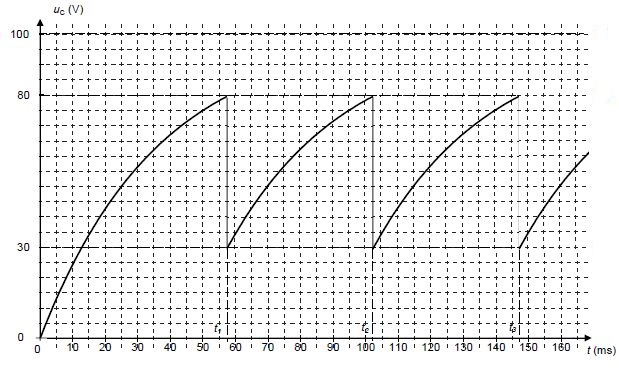
\includegraphics[width=0.65\linewidth]{elec/neon.jpg}
    \caption{Tension au bornes du néon $u_\textsc{c}$ en fonction du temps.}
\end{figure}

\`A $t<0$, le condensateur $C$ est déchargé et le tube est éteint. On allume le générateur à $t=0$.

Le circuit électrique, dans lequel est inséré le tube fluorescent, est schématisé ci-dessous :
\begin{circuit}[Modélisation du tube néon.]
      \draw (0,0)
      to [vsource, v^>=$E$] (0,3)
      to [R, l=$R$] (2,3)
      to [C, l_=$C$, *-*] (2,0)
      to [short] (0,0) {}
      (2,3) to [short] (4,3)
      to [nos, l^=$K$] (4,2)
      to [R, l^=$r$] (4,0)
      to [short] (2,0) {}
      (2.7,0) [open, v_=$u_\textsc{c}$] to (2.7,3) {} ;
      \draw [red, dashed] (3.6,-0.2) rectangle(4.8,3.2) ;
      \node [red] at (4.2,3.5) {Tube néon};
\end{circuit}
Le tube fluorescent est modélisé comme une résistance faible $r$ et un interrupteur $K$ en série. L'interrupteur est ouvert lorsque le tube est éteint et fermé lorsque le tube est allumé.
% Le tube fluorescent est modélisé comme une résistance faible $r$ et un interrupteur $K$ qui s'ouvre et se ferme selon si le tube est allumé ou éteint.

\paragraph{Données :} $E = 100$ V, $R = 60$ k$\Omega$, $r = 10$ $\Omega$, $C = 600$ nF.


\begin{questions}
    \questioncours Condensateurs et dipôles à comportement capacitifs.
    
    \question Décrire le comportement global observé en Fig.~\arabic{exercise}.1 ci-dessus et donner les valeurs de $U_e$ et $U_a$.
    
    \uplevel{On étudie d'abord le circuit entre $t = 0$ et $t_1$.}
    
    \question Simplifier le circuit \arabic{exercise}.1 dans ce cas puis résoudre l'équation différentielle vérifiée par $i$ et $u_\textsc{c}$.
    \question Calculer le temps $t_1$ de l'allumage du néon. Par analogie, quel est le temps $\tau$ du cycle d'allumage du néon ?
    
    \uplevel{On étudie maintenant d'abord le circuit entre $t_1$ et $t_1 + \varepsilon$.}
     
    \question En remarquant que $R\gg r$, simplifier le circuit \arabic{exercise}.1 dans ce cas puis résoudre l'équation différentielle vérifiée par $i$ et $u_\textsc{c}$.
    \question Calculer le temps $t'$ de décharge du condensateur. Justifier que l'on peut négliger ce temps dans le cycle du néon. Voit-on le néon s'allumer et s'éteindre ?
    
\end{questions}
\end{exercise}
% Niveau :      PCSI
% Discipline :  Elec
% Mots clés :   Elec, Ordre 1

\begin{exercise}{Combinaison de dipôles}{1}{Sup}
{\'Electrocinétique, Circuits d'ordre 1}{lelay,mines}

On cherche à décrire le circuit suivant :
\begin{circuit}
      \draw
      node [ground] at (0,0) {}
      to [vsource, v^>=$E$, i^>=$i$] (0,2)
      to [short] (1,2)
      
      (1,2) to [short] (1,1)
      to [short] (2,1)
      to [R, l^=$R_2$] (3,1)
      to [short] (4,1)
      to [short] (4,2)
      
      (1,2) to [short] (1,3)
      to [short] (2,3)
      to [R, l^=$R_1$] (3,3)
      to [short] (4,3)
      to [short] (4,2)
      
      (4,2) to [short] (5,2)
      to [R, l^=$R_0$] (6,2)
      to [short] (7,2)
      
      (7,2) to [short] (8,2)
      
      (8,2) to [short] (8,1)
      to [short] (9,1)
      to [L, l^=$L_2$] (10,1)
      to [short] (11,1)
      to [short] (11,2)
      
      (8,2) to [short] (8,3)
      to [short] (9,3)
      to [L, l^=$L_1$] (10,3)
      to [short] (11,3)
      to [short] (11,2)
      
      (11,2) to [short] (12,2)
      to [L, l^=$L_0$] (13,2)
      to [short] (14,2)
      
      to [short] (14,0)
      node [ground]{};
\end{circuit}

\begin{questions}
    \questioncours Loi de composition des résistances en série et en parallèle. (Si vous l'avez vu : ) Pont diviseur de tension.
    \question Écrire l'équation régissant le courant $i$ passant  dans le circuit plus haut et montrez que cette équation peut se mettre sous la forme
    \begin{align*}
        L \dv{i}{t} + Ri = E
    \end{align*}
    Où $L$ (resp. $R$) est une inductance (resp. résistance) fonction de $L_0$, $L_1$ et $L_2$ (resp. $R_0$, $R_1$, $R_2$) que l'on précisera.
    \question La forme revêtue par $L$ vous semble-t-elle familière ? Justifier que les bobines se comportent `un peu comme' des résistances.
    \question Écrire maintenant l'équation régissant l'évolution de la tension $u$ dans le circuit suivant et montrez que cette équation peut se mettre sous la forme
    \begin{align*}
        C \dv{u}{t} + \frac{u}{R} = I
    \end{align*}
    Où $C$ (resp. $R$) est une capacité (resp. résistance) fonction de $C_0$, $C_1$ et $C_2$ (resp. $R_0$, $R_1$, $R_2$) que l'on précisera.
    
\begin{circuit}
      \draw
      node [ground] at (0,0) {}
      to [short] (0,2)
      to [short] (1,2)
      
      (1,2) to [short] (1,1)
      to [short] (2,1)
      to [R, l^=$R_2$] (3,1)
      to [short] (4,1)
      to [short] (4,2)
      
      (1,2) to [short] (1,3)
      to [short] (2,3)
      to [R, l^=$R_1$] (3,3)
      to [short] (4,3)
      to [short] (4,2)
      
      (4,2) to [short] (5,2)
      to [R, l^=$R_0$] (6,2)
      to [short] (7,2)
      
      node [ground] at (7,0) {}
      (7,0) to [isource, v^>=$u$, i^>=$I$] (7,2)
      
      (7,2) to [short] (8,2)
      
      (8,2) to [short] (8,1)
      to [short] (9,1)
      to [C, l^=$C_2$] (10,1)
      to [short] (11,1)
      to [short] (11,2)
      
      (8,2) to [short] (8,3)
      to [short] (9,3)
      to [C, l^=$C_1$] (10,3)
      to [short] (11,3)
      to [short] (11,2)
      
      (11,2) to [short] (12,2)
      to [C, l^=$C_0$] (13,2)
      to [short] (14,2)
      
      to [short] (14,0)
      node [ground]{};
\end{circuit}

    \question Proposer une loi de composition en série et en parallèle des bobines et des condensateurs.
\end{questions}
\end{exercise}


\begin{solution}

\begin{questions}
    \questioncours ok
    \question $E$
    \question $t = 0$, la bobine est un interrupteur ouvert, $t=\infty$, le condensateur est un fil
    \question $3L \dv{u}{t} + R u = 0$
    \question $\tau = 3L/R$
    \question Une exponentielle décroissante pépère.
\end{questions}

\end{solution}
% Niveau :      PCSI
% Discipline :  Elec
% Mots clés :   Elec, Ordre 1

\begin{exercise}{Bobine avec interrupteur}{1}{Sup}
{\'Electrocinétique, Circuits d'ordre 1}{lelay}

On cherche à décrire le circuit suivant :
\begin{circuit}
      \draw
      node [ground] at (0,0) {}
      to [vsource, v^>=$E$] (0,2)
      to [R, l^=$R$] (2,2)
      to [nos, l=$K$] (4,2)
      to [R, l^=$R$] (6,2)
      to [vsource, v^<=$E$] (6,0)
      node [ground]{}
      (2,2) to [R, l_=$R$] (2,0)
      node [ground]{}
      (4,2) to [L, l^=$L$] (4,0)
      node [ground]{};
\end{circuit}

\begin{questions}
    \questioncours Donne la loi reliant la tension aux bornes d'une bobine au courant qui la traverse. Unité et ordre de grandeur de l'inductance d'une bobine.
    \question Quelle est la tension aux bornes de la bobine tant que l'interrupteur reste ouvert ? Le courant qui la traverse ?
    \question À $t = 0$, on ferme l'interrupteur $K$. Donner le circuit équivalent à $t = 0^+$ et à $t = \infty$.
    \question Donner l'équation différentielle vérifiée par la tension $u$ aux bornes de la bobine.
    \question Quel est le temps caractéristique d'évolution de $u(t)$ ? Quel nom proposez-vous de lui donner ?
    \question Écrire $u(t)$ et donner l'allure de sa courbe.
\end{questions}
\end{exercise}


\begin{solution}

\begin{questions}
    \questioncours ok
    \question $E$
    \question $t = 0$, la bobine est un interrupteur ouvert, $t=\infty$, le condensateur est un fil
    \question $3L \dv{u}{t} + R u = 0$
    \question $\tau = 3L/R$
    \question Une exponentielle décroissante pépère.
\end{questions}

\end{solution}
% Niveau :      PCSI
% Discipline :  Elec
% Mots clés :   Elec, Ordre 1

\begin{exercise}{Condensateur avec interrupteur}{1}{Sup}
{\'Electrocinétique, Circuits d'ordre 1}{lelay}

On cherche à décrire le circuit suivant :
\begin{circuit}
      \draw
      node [ground] at (0,0) {}
      to [vsource, v^>=$E$] (0,2)
      to [R, l^=$R$] (2,2)
      to [nos, l=$K$] (4,2)
      to [R, l^=$R$] (6,2)
      to [vsource, v^<=$E$] (6,0)
      node [ground]{}
      (2,2) to [R, l_=$R$] (2,0)
      node [ground]{}
      (4,2) to [C, l^=$C$] (4,0)
      node [ground]{};
\end{circuit}

\begin{questions}
    \questioncours Donne la loi reliant la tension aux bornes d'un condensateur à la charge qu'il contient. Unité et ordre de grandeur de la capacité d'un condensateur.
    \question Quelle est la tension aux bornes du condensateur tant que l'interrupteur reste ouvert ? Le courant qui le traverse ?
    \question À $t = 0$, on ferme l'interrupteur $K$. Donner le circuit équivalent à $t = 0^+$ et à $t = \infty$.
    \question Donner l'équation différentielle vérifiée par la tension $u$ aux bornes du condensateur.
    \question Quel est le temps caractéristique d'évolution de $u(t)$ ? Quel nom proposez-vous de lui donner ?
    \question Écrire $u(t)$ et donner l'allure de sa courbe.
\end{questions}
\end{exercise}


\begin{solution}

\begin{questions}
    \questioncours ok
    \question $E$
    \question $t = 0$, le condensateur est un fil, $t=\infty$, le condensateur est un interrupteur ouvert
    \question $RC \dv{u}{t} + 3 u = 2e$
    \question $\tau = RC/3$
    \question Une exponentielle saturante pépère.
\end{questions}

\end{solution}
% Niveau :      PCSI - PC
% Discipline :  Elec
% Mots clés :   Elec, Ordre 2

\begin{exercise}{Circuit avec interrupteur}{2}{Sup,Spé}
{\'Electrocinétique, Circuits d'ordre 2}{lelay,mines}

On cherche à décrire le circuit suivant :
\begin{circuit}
      \draw
      node [ground] at (0,0) {}
      to [short] (0,1)
      to [vsource, v^>=$E$] (0,3) 
      to [short] (0,4)
      to [nos, l=$K$] (2,4)
      to [C, l_=$C$, *-*] (2,2)
      to [R, l_=$R$] (2,0)
      node [ground]{}
      (2,4) to [short] (5,4)
      to [R, l^=$R$, -*] (5,2)
      to [C, l^=$C$] (5,0)
      node [ground]{}
      (2,2) to [short, i_=$i$] (3,2) 
      to [R, l^=$R$] (5,2);
\end{circuit}
Initialement, les condensateurs $C$ sont déchargés.

\begin{questions}
    \questioncours Donne la loi reliant la tension aux bornes d'un condensateur à la charge qu'il contient.
    \question On considère le circuit ci-dessus. À $t = 0$, on ferme l'interrupteur $K$. 
    \question Donner le circuit équivalent à $t = 0^+$ et à $t = \infty$.
    \question En déduire $i(t = 0^+)$ et $i(t = \infty)$. Justifier qu'il y a un instant $t_0$ pour lequel $i(t_0) = 0$.
    \question Donner l'équation différentielle vérifiée par $i$ et en déduire $i(t)$.
    \question Donner $t_0$.
\end{questions}
\end{exercise}


\begin{solution}


Par symétrie, la tension aux bornes des deux condensateurs est la même, notée $u$ (si pas convaincu: écrire le système et vérifier que $u_{C_1}-u_{C_2} = 0$).

Du coup (loi des mailles) : la tension aux bornes des deux résistances sur le coté est $u-E$.

On a donc (loi des mailles sur une maille intérieure) : $u + Ri + u-E = 0$ et (loi des noeuds sur un des noeuds) : $i = \frac{u-E}{R} + C\dv{u}{t}$. On en déduit immédiatement que $u = (E-Ri)/2$ et donc que $i$ satisfait $\dv{i}{t} + \frac{3i}{\tau} = \frac{-1}{\tau}\frac{E}{R}$, donc $i(t) = \frac{E}{R}-\frac{4}{3}\frac{E}{R}e^{3t/\tau}$ donc $t_0 = \frac{\tau}{3}\ln\qty(\frac43)$
\begin{circuit}
      \draw
      node [ground] at (0,0) {}
      to [short] (0,1)
      to [vsource, v^>=$E$] (0,3) 
      to [short] (0,4)
      to [short] (2,4)
      to [C, v_<=$u$] (2,2)
      to [R, v_>=$u - E$] (2,0)
      node [ground]{}
      (2,4) to [short] (5,4)
      to [R, v^>=$u - E$] (5,2)
      to [C, v^<=$u$] (5,0)
      node [ground]{}
      (2,2) to [R, v^<=$Ri$] (5,2);
\end{circuit}

\end{solution}
% Niveau :      PCSI
% Discipline :  Elec
% Mots clés :   Elec, Ordre 2

\begin{exercise}{Condensateurs couplés}{2}{Sup}{\'Electrocinétique, Circuits d'ordre 2}{correge}

On considère le schéma suivant. Les condensateurs de même capacité $C$ sont déchargés lorsque les interrupteurs $K_1$ et $K_2$ sont ouverts.

\begin{figure}[H]
\centering
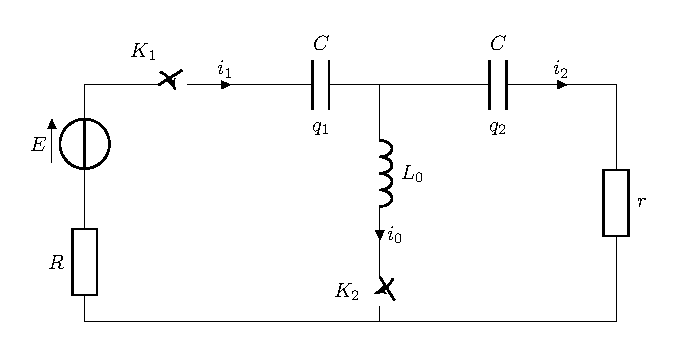
\includegraphics[scale=0.9]{elec/CondCouples.pdf}
\end{figure}

\begin{questions}

    \question En régime continu, par quels éléments peut-on remplacer condensateurs et bobines ?
    \question On ferme $K_1$, $K_2$ restant ouvert. Déterminer en un minimum de calcul  les charges $q_1$ et $q_2$ portées par les deux condensateurs identiques au bout d'un temps très long.
    \question Quelle est alors l'énergie emmagasinée par le système ? \\
              Application numérique pour $C=1\mu$F et $E=10$V.
    \question À partir de maintenant, on ferme $K_2$, $K_1$ restant fermé, et on prend une nouvelle origine des temps.
              Que vaudront l'intensité $i_0$ dans la bobine et les charges $q_1$ et $q_2$ au bout d'un temps long ? \\
              Indication : commencer par dessiner un schéma équivalent au bout d'un temps très long, et raisonner sur ce schéma à l'aide des lois de Kirchhoff.
    \question Quelles sont l'intensité $i_0$ dans la bobine et les charges $q_1$ et $q_2$ des condensateurs à $t=0^+$ ? Justifier.
    \question Écrire les lois de Kirchhoff et les lois usuelles pour les divers composants, puis établir deux équations différentielles du second ordre que vérifient les charges $q_1$ et $q_2$ des deux condensateurs après la fermeture de $K_2$.
    \question On suppose à partir d'ici que $r=R$. Montrer qu'à partir des deux équations différentielles précédentes, on obtient une équation sur $Q=q_1+q_2$ et une équation sur $q=q_1-q_2$.
    \question Résoudre ces équations, donner l'expression de $Q(t)$ et $q(t)$, et montrer en particulier que $Q$ est effectivement indépendante du temps.
    \question Les autres valeurs des composants sont prises à $L_0=5$mH, $r=200\Omega$. \\
              Montrer que 
              \[i_0(t) = \frac{r^2 C E}{16 L_0^2} t\cdot\exp\left(-\frac{r}{4L_0}t\right),\]
              et représenter graphiquement l'allure de $i_0(t)$.
\end{questions}



\end{exercise}

\begin{solution}
\begin{questions}
    \question En régime continu, une bobine est équivalente à un fil, alors qu'un condensateur est équivalent à un interrupteur ouvert.
    \question  Au bout d'un temps long, les condensateurs se comportent comme des coupe-circuits. Le courant circulant dans le circuit est donc nul. Par suite, la loi des mailles donne
                \begin{equation}
                E = u_1+u_2
                \end{equation}
                avec $u_1$ et $u_2$ les tensions aux bornes des condensateurs. Mais comme les deux condensateurs sont reliés par un fil, en régime permanent, la charge portée par leurs armatures est nécessairement la même. D'où $q_1=q_2=q$, et par suite 
                \begin{equation}
                E=2\times\frac{q}{C} \quad \Longrightarrow \quad \boxed{q = \frac{CE}{2}}
                \end{equation}
    \question On a alors l'énergie $W$ emmagasinée par le système
                \begin{equation}
                W = 2\times\frac{1}{2}\frac{q^2}{C} = \frac{CE^2}{4} = 2,5.10^{-5}J
                \end{equation}
    \question Pour un temps long, la bobine est équivalente à un fil. On a toujours $i_1=i_2=0$ car les condensateurs bloquent le courant, et par la loi des noeuds $i_0=0$. 
              En appliquant la loi des mailles dans la maille de gauche, on a $u_1=E$ (pas de tension aux bornes des résistances), donc $q_1=CE$. Dans la maille de droite, $u_2=0$ donc $q_2=0$.
    \question Par continuité de l'intensité traversant une bobine, $i_0(0^+)=0$. Par ailleurs, la charge au borne d'un condensateur est une fonction continue (car la tension l'est), donc on a $q_1(0^+)=q_2(0^+)=\frac{CE}{2}$.
    \question On écrit la loi des mailles dans les mailles de droite et de gauche :
                \begin{align}
                    E &= u_0+u_1+Ri_1 \\
                    0 &= u_0-u_2-ri_2
                \end{align}
                On a bien sûr $i_1=i_0+i_2$. 
                Par ailleurs, $u_1 = \frac{q_1}{C}, u_2=\frac{q_2}{C}$, et finalement:
                \begin{equation}
                    u_0=L_0\dv{i_0}{t}=L_0\dv{(i_1-i_2)}{t} = L_0\left(\dv{ q_1}{t}-\dv{q_2}{t}\right).
                \end{equation}
                En réarrangeant les équations de mailles, on obtient donc les équations différentielles couplées

                \begin{equation}
                \label{eqcouple}
                \boxed{
                \left\{\begin{array}{ll}
                \dv{ q_1}{t}-\dv{ q_2}{t}+\frac{R}{L_0}\dv{q_1}{t}+\frac{q_1}{L_0 C} = \frac{E}{L_0}\\
                \dv{q_1}{t}-\dv{ q_2}{t}-\frac{r}{L_0}\dv{q_2}{t}-\frac{q_2}{L_0 C} = 0 \\
                \end{array}\right.}
                \end{equation}
    \question  Les équations présentées ici sont caractéristiques de ce qu'on appelle des modes symétriques et antisymétriques (vous les retrouverez en TP lors de l'étude des pendules couplés). L'astuce habituelle pour les découpler consiste à faire apparaître les combinaisons $Q=q_1+q_2$ et $q=q_1-q_2$. Puis, prenant (\ref{eqcouple}), et calculant la somme et la différence des deux équations, on obtient finalement

                \begin{equation}
                \boxed{ \left\{\begin{array}{ll}
                    \dv{q}{t}+\frac{r}{2L_0}\dv{q}{t}+\frac{q}{2L_0 C} = \frac{E}{2L_0} \\
                    \dv{Q}{t}+\frac{Q}{rC} = \frac{E}{r} 
                \end{array}\right.}
                \end{equation}
    \question Résolvons l'équation différentielle pour $Q$. Il s'agit d'une équation différentielle du premier ordre avec second membre. La solution de l'équation homogène associée est $Q_H(t) = Ke^{-t/rC}$. Une solution particulière est $Q_p(t) = CE$. La condition initiale est 

                \begin{equation}
                Q(0) = q_1(0)+q_2(0) = CE \Rightarrow K+CE = CE \Rightarrow K=0 !
                \end{equation}

                Ainsi, $\boxed{Q(t)=CE=\text{cste}}$ : la charge totale des deux condensateurs reste constante.

                On résout maintenant l'équation différentielle associée à $q$. Il s'agit d'une équation du second ordre. On commence par résoudre l'équation sans second membre. L'équation caractéristique est
                \[x^2+\frac{r}{2L_0}x+\frac{1}{2L_0C}=0.\]

                Son discriminant vaut $\Delta = \frac{r^2}{4L_0^2}-\frac{2}{L_0C} \approx 0$ avec le degré de précision des données du problème. On a donc une racine double $x=\frac{r}{4L_0}$, et la solution se met sous la forme $q_H(t) = (At+B)\exp\left(-\frac{r}{4L_0}t\right)$. Une solution particulière étant $q_p(t)=CE$, on a alors 

                \begin{equation}
                q(t) = CE+(At+B)\exp\left(-\frac{r}{4L_0}t\right).
                \end{equation}

                Les conditions initiales sont $q(0^+) = q_1(0^+)-q_2(0^+) = 0$, ce qui amène $B=-CE$. Par ailleurs, $\dv{q}{t}(0^+) = \dv{q_1}{t}(0^+)-\dv{q_2}{t}(0^+) = i_1(0^+)-i_2(0^+) = i_0(0^+) = 0$, et $\dv{q}{t} = (A-\frac{r}{4L_0}(At-CE))\exp\left(-\frac{r}{4L_0}t\right) = A+\frac{rCE}{4L_0}$, soit $A=-\frac{rCE}{4L_0}$. Finalement 

                \begin{equation}
                q(t) = CE\left(1-(1+\frac{r}{4L_0}t)e^{-\frac{r}{4L_0}t}\right).
                \end{equation}
    \question On sait que $i_0 = i_1-i_2$, donc $i_0=\dv{q}{t}$, ce qui donne
                \begin{equation}
                    i_0(t)=CE\left(-\frac{r}{4L_0}+\frac{r}{4L_0}(1+\frac{r}{4L_0})\right)\exp(-\frac{r}{4L_0}t)
                \end{equation}
                \begin{equation}
                \boxed{i_0(t) =\frac{r^2CE}{16L_0^2}t.\exp\left(-\frac{r}{4L_0}t\right)}
                \end{equation}
\end{questions}

\end{solution}
% Niveau :      PCSI
% Discipline :  Elec
% Mots clés :   Elec, Ordre 2

\begin{exercise}{Décrement logarithmique}{2}{Sup}{\'Electrocinétique, Circuits d'ordre 2}{correge}

Dans le montage ci-dessous, le générateur de tension est idéal, de force électromotrice $E$ constante. Tant que l'interrupteur est ouvert, le condensateur est déchargé et la bobine (idéale) n'est parcourue par aucun courant. À l'instant $t=0$, on ferme l'interrupteur.

\begin{figure}[H]
\centering
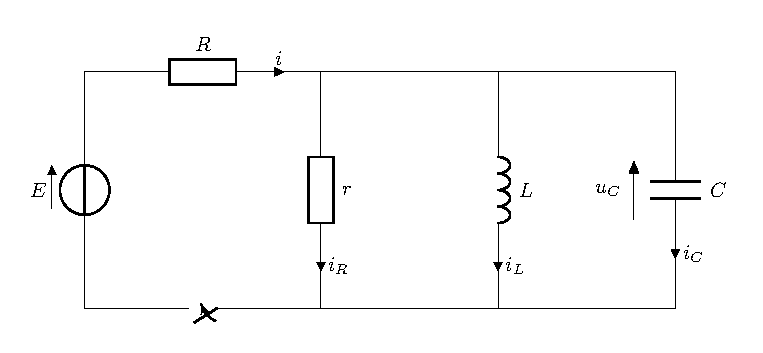
\includegraphics[scale=1]{elec/circuitDecrement.pdf}
\end{figure}

\begin{questions}
    \question Déterminer par raisonnements simples la tension $u$ et les courants $i_R, i_L,i_C$ et $i$ (dans l'ordre qui vous paraîtra le plus judicieux):  à $t=0^-$, à $t=0^+$ et à $t\to \infty$.
    
    \question Établir l'équation différentielle régissant l'évolution de $i_R$ (on pourra écrire la loi des noeuds et la dériver). On posera pour ce circuit parallèle :
              \[\omega_0 = \frac{1}{\sqrt{LC}} \qquad \lambda = \frac{R+r}{2rRC}\]
    \question Pour la suite, on prendra $R=\SI{2,50}{k\ohm}, r=\SI{1,25}{k\ohm}, C=\SI{1,00}{\micro\farad}, L=\SI{20,0}{mH}, E=\SI{6,00}{V}$. À quel type de régime transitoire assiste-t-on ? Justifier.
    \question Définir et calculer la pseudo-pulsation $\omega$ et la pseudo-période $T$ du phénomène. Compte-tenu de la précision des données, que peut-on dire des valeurs numériques comparées de $\omega$ et $\omega_0$ ?
    \question Écrire la solution de l'équation différentielle en $i_R$ obtenue à la question 2 et satisfaisant aux conditions initiales trouvées à la question 1.
    \question En déduire alors l'expression de $u(t)$ et tracer l'allure du graphe correspondant. Donner l'instant $t_0$ auquel $u$ atteint sa valeur maximale.
    \question On définit le décrément logarithmique de $u$ par 
              \[\delta = \frac{1}{n}\ln\left(\frac{u(t)}{u(t+nT)}\right)\]
              Exprimer $\delta$ en fonction de $\lambda$ et $T$. Application numérique.
\end{questions}
\end{exercise}

%vides ?
%\input{elec/ALI}
%\input{elec/autourdurlc}


\section{\'Electronique en régime sinusoïdal forcé}
\begin{exercise}{Quelques (pré) filtres (1)}{1}{Sup}
{\'Electrocinétique}{lelay}

\begin{questions}
    \questioncours Notion de déphasage, d'avance et de retard de phase
    \question Donner le déphasage entre $\underline{s}$ et $\underline{e}$ dans le circuit suivant en fonction de la fréquence $\omega$ de $\underline{e}$
\begin{circuit}
      \draw
      (0,0) to [open, v_=$\underline{e}$, *-o] (0,2)
      (0,2) to [R, l=$R$] (2,2) 
      to [C, l^=$C$, *-*] (2,0)
      (2,2) to [short] (4,2)
      (4,0) to [open, v_=$\underline{s}$, *-o] (4,2)
      (0,0) to [short] (4,0);
\end{circuit}
    \question Pour quelle valeur de $\omega$ a-t-on un déphasage de $-\pi/3$ ?
    \question Tracer la courbe $\Delta\varphi = f(\omega)$
    \question Donner le déphasage entre $\underline{s}$ et $\underline{e}$ dans le circuit suivant en fonction de la fréquence $\omega$ de $\underline{e}$
\begin{circuit}
      \draw
      (0,0) to [open, v_=$\underline{e}$, *-o] (0,2)
      (0,2) to [R, l=$R$] (2,2) 
      to [L, l^=$L$, *-*] (2,0)
      (2,2) to [short] (4,2)
      (4,0) to [open, v_=$\underline{s}$, *-o] (4,2)
      (0,0) to [short] (4,0);
\end{circuit}
    \question Pour quelle valeur de $\omega$ a-t-on un déphasage de $\pi/3$ ?
    \question Tracer la courbe $\Delta\varphi = f(\omega)$
    \question Que remarquez-vous ?
\end{questions}

\end{exercise}

\begin{exercise}{Quelques (pré) filtres (2)}{1}{Sup}
{\'Electrocinétique}{lelay}

\begin{questions}
    \questioncours Passage en complexe : signification, limitations
    \question Donner le déphasage entre $\underline{s}$ et $\underline{e}$ dans le circuit suivant en fonction de la fréquence $\omega$ de $\underline{e}$
\begin{circuit}
      \draw
      (0,0) to [open, v_=$\underline{e}$, *-o] (0,2)
      (0,2) to [C, l=$C$] (2,2) 
      to [R, l^=$R$, *-*] (2,0)
      (2,2) to [short] (4,2)
      (4,0) to [open, v_=$\underline{s}$, *-o] (4,2)
      (0,0) to [short] (4,0);
\end{circuit}
    \question Pour quelle valeur de $\omega$ a-t-on un déphasage de $\pi/3$ ?
    \question Tracer la courbe $\Delta\varphi = f(\omega)$
    \question Donner le déphasage entre $\underline{s}$ et $\underline{e}$ dans le circuit suivant en fonction de la fréquence $\omega$ de $\underline{e}$
\begin{circuit}
      \draw
      (0,0) to [open, v_=$\underline{e}$, *-o] (0,2)
      (0,2) to [L, l=$L$] (2,2) 
      to [R, l^=$R$, *-*] (2,0)
      (2,2) to [short] (4,2)
      (4,0) to [open, v_=$\underline{s}$, *-o] (4,2)
      (0,0) to [short] (4,0);
\end{circuit}
    \question Pour quelle valeur de $\omega$ a-t-on un déphasage de $-\pi/3$ ?
    \question Tracer la courbe $\Delta\varphi = f(\omega)$
    \question Que remarquez-vous ?
\end{questions}

\end{exercise}

 % Niveau :      PCSI - PC
% Discipline :  Elec
% Mots clés :   Elec, Ordre 2

\begin{exercise}{Bobine réelle}{1}{Sup,Spé}
{\'Electrocinétique, Circuits d'ordre 2}{lelay,centrale}

Dans cet exercice, on cherche à étudier les caractéristique d'une bobine réelle (par opposition à une bobine idéale).

\begin{questions}
    \questioncours Composants élémentaires en électrocinétique et ordres de grandeur.
    \question En quoi consiste une bobine réelle (dans la vraie vie, par opposition à bobine "idéale") ? Justifier qu'on représente une bobine réelle par une bobine parfaite et une résistance en série.
    \question On s'intéresse au circuit suivant. A l'aide d'une étude asymptotique, trouver quel filtre est ici réalisé.

\begin{circuit}
      \draw
      node [ground] at (0,0) {}
      (0,0) to [sV, v^>=$U_e$] (0,2)
            to [R, l=$r$] (2,2)
            to [L, l=$L$] (4,2)
            to [C, l=$C$] (6,2)
            to [R, l_=$R$, v^<=$U_s$] (6,0)
            to [short]    (0,0);
      \draw [red, dashed] (0.2,1.5) rectangle(3.8,2.8) ;
      \node [red] at (2.0,3.1) {Bobine réelle};
\end{circuit}
    
    \question Sur l'écran d'un oscilloscope mesurant $U_s$ et $U_e$ on voit le graphe représenté ci dessous. Quelle est la fréquence de ces signaux ? Quel est leur décalage en amplitude ? En phase ?

\begin{figure}[H]
    \centering
    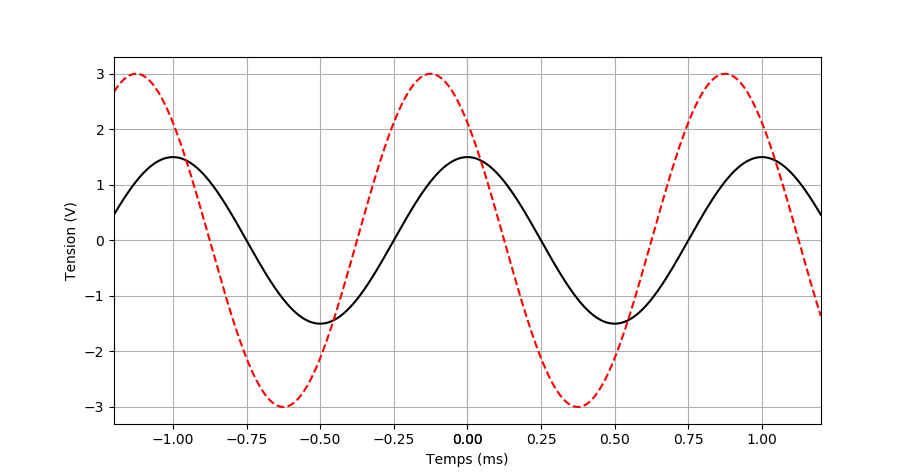
\includegraphics[width=\linewidth]{elec/filtragelineaire/OSCILLO_DECALE.png}
    \caption{En rouge et en tirets : $U_e$ (l'excitation), en noir : $U_s$ (la réponse).}
\end{figure}

    \question Sachant qu'on sait que $C = 1.00$ $\mu$F et $R =1.00$ k$\Omega$, donner la valeur de $L$ et de $r$. Conclure sur la qualité de la bobine utilisée.
\end{questions}
\end{exercise}

\begin{solution}

\begin{questions}
    \questioncours Parler un peu de C et L en vrai, OdG genre 1 nF et 10 mH
    \question C'est un long fil donc normal résistance
    \question Passe-bande
    \question Fréquence : $\omega = 1 kHz$, décalage en amplitude : facteur 1/2, décalage en fréquence : -pi/4 donc $H(\omega) = \frac12e^{-i\pi/4}$
    \question La fonction de transfert est bien sur $H(\omega) = \frac1{1+\frac{r}R + j\frac1R\qty(L\omega-\frac{1}{C\omega})}$. On utilise la phase d'abord : 
    \begin{align*}
    arg\qty(\frac1{1+\frac{r}R + j\frac1R\qty(L\omega-\frac{1}{C\omega})}) = -arg\qty( 1+\frac{r}R + j\frac1R\qty(L\omega-\frac{1}{C\omega}) ) = -\frac{\pi}4 \\
    \arctan\qty(\frac{\frac1R\qty(L\omega-\frac{1}{C\omega})}{1+\frac{r}R}) = \frac{\pi}4 \\
    \frac{\frac1R\qty(L\omega-\frac{1}{C\omega})}{1+\frac{r}R} = 1 \\
    \frac1R\qty(L\omega-\frac{1}{C\omega}) = 1+\frac{r}R
    \end{align*}
    Ensuite, l'amplitude :
    \begin{align*}
    \abs{\frac1{1+\frac{r}R + j\frac1R\qty(L\omega-\frac{1}{C\omega})}} = \frac1{\abs{1+\frac{r}R + j\frac1R\qty(L\omega-\frac{1}{C\omega})}} = \frac12\\
    \abs{1+\frac{r}R + j\frac1R\qty(L\omega-\frac{1}{C\omega})} = 2 \\
    \sqrt{\qty(1+\frac{r}R)^2 + \frac1R\qty(L\omega-\frac{1}{C\omega})^2} = 2
    \end{align*}
    On utilise le résultat sur la phase
    \begin{align*}
    \sqrt{2}\qty(1+\frac{r}R) = 2 \\
    1+\frac{r}R = \sqrt{2} \\
    r = R(\sqrt{2} -1)
    \end{align*}
    Et on repart du résultat sur la phase
    \begin{align*}
    \frac1R\qty(L\omega-\frac{1}{C\omega}) = \sqrt{2} \\
    L = \frac{R\sqrt{2}}{\omega} + \frac1{C\omega^2}
    \end{align*}
    Donc voilà
    
\end{questions}

\end{solution}

\begin{exercise}{Usine alimentée par un courant sinusoïdal}{1}{Sup}{\'Electrocinétique,Régime sinusoidal forcé}{correge}

\begin{questions}
    \questioncours Montrer le lien entre valeur efficace et amplitude pour un signal sinusoïdal.

    \uplevel{Une usine, alimentée sous la tension sinusoïdale de valeur efficace $U=\SI{220}{V}$ et de fréquence $f=\SI{50}{Hz}$, consomme une puissance moyenne $P=\SI{100}{kW}$; son facteur de puissance est $\cos \phi=0.8$.}
    
    \question Calculer l'intensité efficace $I$. \\ On pourra montrer que $P$ ne dépend que de $U$ et $I$ et $\cos\phi$, $\phi$ étant le déphasage entre $u(t)$ et $i(t)$.

    \uplevel{Souvent, les installations industrielles et domestriques ont un caractère inductif (\emph{i.e.} se comportent comme une inductance résistive), lié à la présence de fils et de bobinages (moteurs, transformateurs~\emph{etc.}).}

    \question Représenter qualitativement dans le plan complexe $\ubar{u}$ et $\ubar{i}$ en prenant comme référence la phase de $\ubar{u}$, ainsi que l'argument $\varphi$ de l'impédance équivalente $\ubar{Z}$ de l'usine.

    \question EDF facture à l'usine la puissance moyenne consommée $P$. Sachant que le réseau pour acheminer l'électricité possède une résistance $R_\textsc{edf}$, quelle puissance $P_\text{f}$ doit fournir EDF en fonction de $P$, $R_\textsc{edf}$ et $I$ ? Que doit valoir $\phi$ pour réduire la charge sur le réseau ?
    
    \uplevel{EDF met en parallèle avec l'usine un condensateur de capacité $C$ de sorte que le facteur de puissance $\cos\phi_\text{tot}$ de l'ensemble soit maximal.}

    \question Compléter la figure de la question 3 en y représentant les amplitudes complexes de $\ubar{i}_C$ et $\ubar{i}_\text{tot}$.

    \question Que doit valoir $C$ pour que le facteur de puissance $\cos\phi = 1$ ? Calculer en pourcentage l'économie réalisée par le fournisseur de l'énergie électrique, l'industriel consommant toujours la même puissance.
\end{questions}
\end{exercise}

\begin{solution}
    \begin{questions}
        \question La valeur efficace est telle que :
        $$U^2 = \ev{u(t)^2} = {u_0}^2 \ev{\cos^2(\omega t)} = \dfrac{1}{2}{u_0}^2 \ev{1 + \cos(2\omega t)} = \dfrac{{u_0}^2}{2}.$$
        D'où $U = u_0/\sqrt{2}$.

        \question $P = \ev{u(t) i(t)} = 2 UI\ev{\cos(\omega t)\cos(\omega t + \phi)} = UI\ev{\cos\phi + \cos(2\omega t + \phi)} = UI\cos\phi$.

        AN. : $I = 568$ A.

        \question $\ubar{u} = \ubar{Z}\, \ubar{i}$, donc $u_0 = Z_0 i_0 e^{j(\phi + \varphi)}$, ce qui indique que $\varphi = -\phi$, l'angle entre $(Ox)$ et $\ubar{i}$. Comme $\ubar{Z} = R + jL\omega$, $0 < \varphi < \pi/2$ et donc $0 > \phi > -\pi/2$, quart bas droite du plan complexe.

        Ainsi $\cos\phi \ll 1$ : on diminue la puissance consommée.

        \question $$P_\text{f} = R_\textsc{edf} I^2 + \abs{Z}\cos\phi I^2 = \dfrac{R_\textsc{edf} I^2 + \abs{Z}\cos\phi}{\cos^2\phi}\dfrac{P^2}{U^2}.$$
        Ainsi pour une même puissance, la charge sur réseau diverge quand $\cos\phi = 0$, EDF tente donc d'optimiser en prenant $\phi = 0$.

        \question $\ubar{i}_C = jC\omega \ubar{u}$ sera donc dans l'axe $Oy$.
        
        $\ubar{i}_\text{tot} = \ubar{i} + \ubar{i}_C = j\qty(C\omega - \dfrac{1}{Z_0}\sin\varphi) + \dfrac{1}{Z_0}\cos\varphi\ubar{u}$ sera entre les deux.

        Pour que $\phi_\text{tot} = 0$, il faut que $\text{Im }\ubar{i}_C = - \text{Im }\ubar{i}$ soit $I_C = I \sin\varphi$ ou encore $C\omega = \dfrac{1}{Z_0}\sin\varphi$.

        \question Ainsi $C = \dfrac{\sin\varphi}{Z_0\omega}$. L'industriel économise donc d'un facteur $\dfrac{1 - \cos\phi}{\cos\phi} = 25\%$.
        
    \end{questions}
\end{solution}
% Niveau :      PCSI - PC
% Discipline :  Elec
% Mots clés :   Elec, Ordre 2

\begin{exercise}{Oscillateur de Van Der Pol}{1}{Sup,Spé}
{\'Electrocinétique, Circuits d'ordre 2}{lelay}

On considère le circuit suivant :
\begin{circuit}
      \draw (0,0)
      to [C, l=$C$] (0,2)
      to [L, l_=$L$] (3,2)
      to [short] (3,0)
      to [vsourcesin, l^=$T$] (.5,0) {}
      to [short, i^<=$i$] (0,0) ;
\end{circuit}
où $T$ est un composant ayant comme loi de courant
$$u_\textsc{t}(i) = -R_0 i_0 \qty[\dfrac{i}{i_0} - \dfrac{1}{3}\qty(\dfrac{i}{i_0})^3].$$

\begin{questions}
    \questioncours Donner les conditions nécessaires à vérifier pour pouvoir passer en notation complexe. Est-il possible de le faire ici ?
    \question Tracer la caractéristique de $T$. Comment qualifier ce composant ?
    \question Montrer que l'équation différentielle vérifiée par $i$ peut se mettre sous la forme
    $$\dv[2]{i}{t} + \dfrac{\omega_0}{Q}\qty[\qty(\dfrac{i}{i_0})^2 - 1]\dv{i}{t} + {\omega_0}^2 i = 0$$
    \question Discuter de l'évolution du système lorsque $i$ est petit / grand devant $i_0$. De façon générale, que va-t-il se passer ?
    \question Que vaut $\En$, la quantité d'énergie contenue dans la bobine et le condensateur ? A votre avis, est-elle conservée ?
    \question On définit $\ev{\En} = \dfrac{1}{T} \displaystyle\int_0^T\En(t)\dd{t}$. Que représente cette quantité ?
    \question On considère une solution périodique $i(t) = \sum_{k=0}^N I_k \cos(k\omega t)$. Montrer qu'alors $\ev{\En}$ est constant (et ne diverge pas à une certaine condition à préciser sur les $I_k$) et donner sa valeur. 
\end{questions}
\end{exercise}

\begin{solution}

\begin{questions}
    \questioncours Faut que tout soit linéaire, $T$ ne l'est aps donc non. 
    \question La focntion $u = f(i)$ est comme $-i$ au voisinage de 0 et comme $i^3$ à l'infini.
    \question Il faut faire une loi des mailles et dériver, on tombe direct sur le bon truc.
    \question POUR LES SUPS : leur dire d'oublier le terme en dérivée seconde pour cette question. POUR LES SPES : faire une analogie avec l'oscillateur harmonique amorti. Quand $i$ est petit (devant $i_0$), on a un terme de frottement négatif, donc $i$ est amplifié et va grandir exponentiellement. Quand $i$ est grand (devant $i_0$), le terme de frottement est positif et augmente avec $\abs{i}$ : $i$ va décroître exponentiellement. Quand $i$ est de l'ordre de $i_0$, on a presque un oscillateur harmonique.
    \question $E_n = \frac12 Li^2 + \frac12 Cu^2$ et n'a aucune raison particulière d'être conservée (surtout vu la question d'avant, le terme de frottement est important).
    \question C'est la moyenne temporelle de l'énergie
    \question L'idée est que si $i$ est périodique on s'en sort avec l'orthogonalité des fonctions trigo.
    \begin{align*}
        \ev{i^2} &= \ev{\qty(\sum_{k=0}^N I_k \cos(k\omega t))^2} \\
            &= \sum_{k=0}^N\sum_{p=0}^N I_k I_p \ev{\cos(k\omega t)\cos(p\omega t)} \\
         &= \sum_{k=0}^N I_k^2 \ev{\cos^2(k\omega t)} + \sum_{k=0}^N\sum_{p\neq k} I_k I_p \ev{\cos(k\omega t)\cos(p\omega t)} \\
        &= \frac12\sum_{k=0}^N I_k^2 + 0
    \end{align*}
    Ce qui ne diverge pas si $(I_k)$ est de carré sommable. On obtient 
    \begin{align*}
        \ev{E_n} &= \frac14 L \sum_k I_k^2 + \frac14 C \sum_k \qty(\frac{I_k}{k})^2
    \end{align*}
\end{questions}
\end{solution}

\section{Filtrage linéaire --- Premier ordre}
% RC passe bas
\begin{exercise}{Filtres linéaires du premier ordre}{0}{Sup}
{\'Electrocinétique,Filtrage linéaire, Premier ordre}{bermudez}

\begin{minipage}[t]{.3\linewidth}
\vspace{-1.5em}
\begin{circuitikz}
      \draw
      (0,0) to [open, v^=$\underline{e}$, *-o] (0,2)
      (0,2) to [R, l=$R$] (2,2) 
      to [C, l^=$C$, *-*] (2,0)
      (2,2) to [short] (3,2)
      (3,0) to [open, v_=$\underline{s}$, *-o] (3,2)
      (0,0) to [short] (3,0);
\end{circuitikz}
\vspace{1em}
\end{minipage}\begin{minipage}[t]{.7\linewidth}
    \textsf{Question de cours : } Déterminez la nature et le diagramme de Bode de ce filtre, en précisant sa fréquence de coupure et son gain statique.
\end{minipage}
\end{exercise}


% RL passe haut
\begin{exercise}{Filtres linéaires du premier ordre}{0}{Sup}
{\'Electrocinétique,Filtrage linéaire, Premier ordre}{bermudez}

\begin{minipage}[t]{.3\linewidth}
\vspace{-1.5em}
\begin{circuitikz}
      \draw
      (0,0) to [open, v^=$\underline{e}$, *-o] (0,2)
      (0,2) to [R, l=$R$] (2,2) 
      to [L, l^=$L$, *-*] (2,0)
      (2,2) to [short] (3,2)
      (3,0) to [open, v_=$\underline{s}$, *-o] (3,2)
      (0,0) to [short] (3,0);
\end{circuitikz}
\vspace{1em}
\end{minipage}\begin{minipage}[t]{.7\linewidth}
    \textsf{Question de cours : } Déterminez la nature et le diagramme de Bode de ce filtre, en précisant sa fréquence de coupure et son gain statique.
\end{minipage}
\end{exercise}


% RC passe bas
\begin{exercise}{Filtres linéaires du premier ordre}{0}{Sup}
{\'Electrocinétique,Filtrage linéaire, Premier ordre}{bermudez}

\begin{minipage}[t]{.3\linewidth}
\vspace{-1.5em}
\begin{circuitikz}
      \draw
      (0,0) to [open, v^=$\underline{e}$, *-o] (0,2)
      (0,2) to [C, l=$C$] (2,2) 
      to [R, l^=$R$, *-*] (2,0)
      (2,2) to [short] (3,2)
      (3,0) to [open, v_=$\underline{s}$, *-o] (3,2)
      (0,0) to [short] (3,0);
\end{circuitikz}
\vspace{1em}
\end{minipage}\begin{minipage}[t]{.7\linewidth}
    \textsf{Question de cours : } Déterminez la nature et le diagramme de Bode de ce filtre, en précisant sa fréquence de coupure et son gain statique.
\end{minipage}
\end{exercise}


% RL passe haut
\begin{exercise}{Filtres linéaires du premier ordre}{0}{Sup}
{\'Electrocinétique,Filtrage linéaire, Premier ordre}{bermudez}

\begin{minipage}[t]{.3\linewidth}
\vspace{-1.5em}
\begin{circuitikz}
      \draw
      (0,0) to [open, v^=$\underline{e}$, *-o] (0,2)
      (0,2) to [L, l=$L$] (2,2) 
      to [R, l^=$R$, *-*] (2,0)
      (2,2) to [short] (3,2)
      (3,0) to [open, v_=$\underline{s}$, *-o] (3,2)
      (0,0) to [short] (3,0);
\end{circuitikz}
\vspace{1em}
\end{minipage}\begin{minipage}[t]{.7\linewidth}
    \textsf{Question de cours : } Déterminez la nature et le diagramme de Bode de ce filtre, en précisant sa fréquence de coupure et son gain statique.
\end{minipage}
\end{exercise}


% Tableau des solutions

{
\def\thesolution{Solutions \arabicAlph{part}\arabicAlph{section}\hspace{2pt}01--\twodigits{exercise}\quad---\quad}
\begin{solution}

\newcounter{subsol}
\newcommand{\parti}{\large\bfseries\sffamily\stepcounter{subsol}\arabicAlph{part}\arabicAlph{section}\hspace{2pt}\twodigits{subsol}\quad}

\noindent\begin{tabularx}{\linewidth}{@{\parti}C@{\vspace{1em}}Ccp{5em}}

\begin{circuitikz}[baseline={(0,2)}]
      \draw
      (0,0) to [open, v^=$\underline{e}$, *-o] (0,2)
      (0,2) to [R, l=$R$] (2,2) 
      to [C, l^=$C$, *-*] (2,0)
      (2,2) to [short] (3,2)
      (3,0) to [open, v_=$\underline{s}$, *-o] (3,2)
      (0,0) to [short] (3,0);
\end{circuitikz} &
$ \underline{H}(\omega) = \dfrac{1}{1+j RC\omega}$ &
Passe-bas &
$H_0 = 1$, \newline $\omega_\text{c} = \dfrac{1}{RC}$ \\

\begin{circuitikz}[baseline={(0,2)}]
      \draw
      (0,0) to [open, v^=$\underline{e}$, *-o] (0,2)
      (0,2) to [R, l=$R$] (2,2) 
      to [L, l^=$L$, *-*] (2,0)
      (2,2) to [short] (3,2)
      (3,0) to [open, v_=$\underline{s}$, *-o] (3,2)
      (0,0) to [short] (3,0);
\end{circuitikz} &
$ \underline{H}(\omega) = \dfrac{j L/R\omega}{1+j L/R\omega}$ &
Passe-haut &
$H_0 = 1$, \newline $\omega_\text{c} = \dfrac{R}{L}$ \\

\begin{circuitikz}[baseline={(0,2)}]
      \draw
      (0,0) to [open, v^=$\underline{e}$, *-o] (0,2)
      (0,2) to [C, l=$C$] (2,2) 
      to [R, l^=$R$, *-*] (2,0)
      (2,2) to [short] (3,2)
      (3,0) to [open, v_=$\underline{s}$, *-o] (3,2)
      (0,0) to [short] (3,0);
\end{circuitikz} &
$ \underline{H}(\omega) = \dfrac{jRC\omega}{1+j RC\omega}$ &
Passe-haut &
$H_0 = 1$, \newline $\omega_\text{c} = \dfrac{1}{RC}$ \\

\begin{circuitikz}[baseline={(0,2)}]
      \draw
      (0,0) to [open, v^=$\underline{e}$, *-o] (0,2)
      (0,2) to [L, l=$L$] (2,2) 
      to [R, l^=$R$, *-*] (2,0)
      (2,2) to [short] (3,2)
      (3,0) to [open, v_=$\underline{s}$, *-o] (3,2)
      (0,0) to [short] (3,0);
\end{circuitikz} &
$ \underline{H}(\omega) = \dfrac{1}{1+j L/R\omega}$ &
Passe-bas &
$H_0 = 1$, \newline $\omega_\text{c} = \dfrac{R}{L}$ \\

\end{tabularx}

\end{solution}

}

% Niveau :      PCSI
% Discipline :  Elec
% Mots clés :   Elec, Ordre 1

\begin{exercise}{Bobine réelle}{1}{Sup}
{\'Electrocinétique, Circuits d'ordre 1}{lelay}

\begin{questions}
    \questioncours Donne la loi reliant la tension aux bornes d'une bobine au courant qui la traverse, sous forme différentielle et complexe. Unité et ordre de grandeur de l'inductance d'une bobine.
    \question La bobine "idéale" existe-t-elle dans la vraie vie ? Justifie qu'on représente une bobine "réelle" par une bobine idéale et un résistance $r$ en série. Comment doit être $r$ afin de se rapproche le plus possible de la bobine idéale ?
    \question On cherche maintenant à trouver l'inductance d'une certaine bobine, en prenant en compte sa résistance interne. On considère le circuit ci-dessous, où $R$ vaut 100 $\Omega$ :
    \begin{circuit}
          \draw
          (0,0) to [open, v_=$\underline{e}$, *-o] (0,2)
          (0,2) to [R, l=$r$] (2,2) 
                to [L, l=$L$] (4,2)
                to [R, l=$R$] (4,0)
          (4,2) to [short] (6,2)
          (6,0) to [open, v_=$\underline{s}$, *-o] (6,2)
          (0,0) to [short] (6,0);
    \end{circuit}
    Donner sa fonction de transfert $\underline{H} = \frac{\underline{s}}{\underline{e}}$
    \question Tracer l'allure du graphe de $\abs{\underline{H}}$ et $\arg(\underline{H})$ en fonction de $\frac{\omega}{\omega_0}$ où $\omega_0$ est une pulsation caractéristique du système que l'on précisera.
    \question Si on se place à très basse fréquence et que le signal d'entrée $\underline{e}$ a une amplitude de 6 V, le signal de sortie présente une amplitude de 5 V. En déduire la valeur de $r$.
    \question On constate qu'à $f = 2.4$ kHz, les deux signaux $\underline{s}$ et $\underline{e}$ sont en quadrature de phase. En déduire la valeur de l'inductance $L$.
\end{questions}
\end{exercise}


\begin{solution}


\begin{questions}
    \questioncours $U = L\dv{i}{t}$, $L\sim 10$ mH
    \question Impossible ideale, une bobine est faite de fil long donc au bout d'un moment on doit avoir de la résistance. idéale : résistance nul du fil, donc $r=0$.
    \question On a un diviseur de tension : 
    $$ \underline{s} = \frac{R}{R\,+\,r + jL\omega}\underline{e}$$
    soit sous forme canonique
    $$ H(\omega) = \frac{H_0}{1 + j\frac{\omega}{\omega_0}}$$
    avec $H_0 = R/(R+r)$ et $\omega_0 = (R+r)/L$
    \question On a un passe bas d'ordre 1, avec une phase qui va de 0 à $-\pi/2$
    \question À très basse fréquence on $H = H_0 = 5/6$ d'où $r = R/5 = 20$ $\Omega$
    \question quadrature de phase : on a $\omega = \omega_0$. On en déduit $L = (R+r)/(2\pi f)$ soit 8 mH.
\end{questions}

\end{solution}
% Niveau :      PCSI
% Discipline :  Elec
% Mots clés :   Elec, Ordre 1

\begin{exercise}{Condensateur réel}{1}{Sup}
{\'Electrocinétique, Circuits d'ordre 1}{lelay}

\begin{questions}
    \questioncours Donne la loi reliant la tension aux bornes d'un condensateur au courant qui le traverse, sous forme différentielle et complexe. Unité et ordre de grandeur de la capacité d'un condensateur
    \question Le condensateur "idéal" existe-t-il dans la vraie vie ? Justifie qu'on représente un condensateur "réel" par un condensateur idéal et une résistance $r$ en parallèle. Comment doit être $r$ afin de se rapproche le plus possible du condensateur idéal ?
    \question On cherche maintenant à trouver la capcité $C$ d'un certain condensateur, en prenant en compte sa résistance interne. On considère le circuit ci-dessous, où $R$ vaut 50 k$\Omega$ :
    \begin{circuit}
          \draw
          (0,0) to [open, v_=$\underline{e}$, *-o] (0,4)
          (0,4) to [R, l=$R$] (2,4) 
                to [short] (4,4)
                to [short] (4,3)
          (4,3) to [short] (5,3)
                to [R, l=$r$] (5,1)
                to [short] (4,1)
          (4,3) to [short] (3,3)
                to [C, l=$C$] (3,1)
                to [short] (4,1)
          (4,1) to [short] (4,0)
          (4,4) to [short] (6,4)
          (6,0) to [open, v_=$\underline{s}$, *-o] (6,4)
          (0,0) to [short] (6,0);
    \end{circuit}
    Donner sa fonction de transfert $\underline{H} = \frac{\underline{s}}{\underline{e}}$
    \question Tracer l'allure du graphe de $\abs{\underline{H}}$ et $\arg(\underline{H})$ en fonction de $\frac{\omega}{\omega_0}$ où $\omega_0$ est une pulsation caractéristique du système que l'on précisera.
    \question Si on se place à très basse fréquence et que le signal d'entrée $\underline{e}$ a une amplitude de 5.25 V, le signal de sortie présente une amplitude de 5 V. En déduire $r$.
    \question On constate qu'à $f = 16$ kHz, les deux signaux $\underline{s}$ et $\underline{e}$ sont en quadrature de phase. En déduire la valeur de la capacité $C$.
\end{questions}
\end{exercise}


\begin{solution}


\begin{questions}
    \questioncours $i = C\dv{U}{t}$, $C\sim 1$ $\mu$H
    \question Impossible ideal, un condensateur est fait d'un milieu isolant mais y a bien une fuite (resistivite non nulle). idéal : résistivite nulle de l'isolant, donc $r=\infty$.
    \question On a un diviseur de tension : 
    \begin{align*}
        \underline{s} &= \frac{\frac{1}{\frac{1}{r} + jC\omega}}{R\,+\,\frac{1}{\frac{1}{r} + jC\omega}}\underline{e} \\
        &= \frac{1}{\frac{R}{r} + jCR\omega + 1}\underline{e}
    \end{align*}     
    soit sous forme canonique
    $$ H(\omega) = \frac{H_0}{1 + j\frac{\omega}{\omega_0}}$$
    avec $H_0 = r/(r+R)$ et $\omega_0 = (R+r)/(rRC)$
    \question On a un passe bas d'ordre 1, avec une phase qui va de 0 à $-\pi/2$
    \question À très basse fréquence on $H = H_0 = 5/5.25$ d'où $r = 20 R = 1$ M$\Omega$
    \question quadrature de phase : on a $\omega = \omega_0$. On en déduit $C = (R+r)/(r R 2\pi f)$ soit 10 $\mu$F.
\end{questions}

\end{solution}

\section{Filtrage linéaire --- Second ordre}
% RLC passe bas 
\begin{exercise}{RLC série}{0}{Sup}
{\'Electrocinétique,Filtrage linéaire, Second ordre}{bermudez}

\begin{minipage}[t]{.4\linewidth}
\vspace{-1.5em}
\begin{circuitikz}
      \draw
      (0,0) to [open, v^=$\underline{e}$, *-o] (0,2)
      (0,2) to [R, l=$R$] (2,2)
      to [L, l=$L$] (4,2) 
      to [C, l^=$C$, *-*] (4,0)
      (4,2) to [short] (5,2)
      (5,0) to [open, v_=$\underline{s}$, *-o] (5,2)
      (0,0) to [short] (5,0);
\end{circuitikz}
\vspace{1em}
\end{minipage}\begin{minipage}[t]{.6\linewidth}
    \textsf{Question de cours : } Déterminez la nature et le diagramme de Bode de ce filtre, en précisant sa fréquence propre, sa fréquence de de résonance, son gain statique / à la résonance, et son facteur de qualité.
\end{minipage}
\end{exercise}



% RLC passe bande 
\begin{exercise}{RLC série}{0}{Sup}
{\'Electrocinétique,Filtrage linéaire, Second ordre}{bermudez}

\begin{minipage}[t]{.4\linewidth}
\vspace{-1.5em}
\begin{circuitikz}
      \draw
      (0,0) to [open, v^=$\underline{e}$, *-o] (0,2)
      (0,2) to [L, l=$L$] (2,2)
      to [C, l=$C$] (4,2) 
      to [R, l^=$R$, *-*] (4,0)
      (4,2) to [short] (5,2)
      (5,0) to [open, v_=$\underline{s}$, *-o] (5,2)
      (0,0) to [short] (5,0);
\end{circuitikz}
\vspace{1em}
\end{minipage}\begin{minipage}[t]{.6\linewidth}
    \textsf{Question de cours : } Déterminez la nature et le diagramme de Bode de ce filtre, en précisant sa fréquence propre, sa fréquence de de résonance, son gain statique / à la résonance, et son facteur de qualité.
\end{minipage}
\end{exercise}



% RLC passe haut 
\begin{exercise}{RLC série}{0}{Sup}
{\'Electrocinétique,Filtrage linéaire, Second ordre}{bermudez}

\begin{minipage}[t]{.4\linewidth}
\vspace{-1.5em}
\begin{circuitikz}
      \draw
      (0,0) to [open, v^=$\underline{e}$, *-o] (0,2)
      (0,2) to [R, l=$R$] (2,2)
      to [C, l=$C$] (4,2) 
      to [L, l^=$L$, *-*] (4,0)
      (4,2) to [short] (5,2)
      (5,0) to [open, v_=$\underline{s}$, *-o] (5,2)
      (0,0) to [short] (5,0);
\end{circuitikz}
\vspace{1em}
\end{minipage}\begin{minipage}[t]{.6\linewidth}
    \textsf{Question de cours : } Déterminez la nature et le diagramme de Bode de ce filtre, en précisant sa fréquence propre, sa fréquence de de résonance, son gain statique / à la résonance, et son facteur de qualité.
\end{minipage}
\end{exercise}




% Tableau des solutions

{
\def\thesolution{Solutions \arabicAlph{part}\arabicAlph{section}\hspace{2pt}01--\twodigits{exercise}\quad---\quad}
\begin{solution}
\ifx\thesubsol\undefined
    \newcounter{subsol}
 \else
    \setcounter{subsol}{-1}
 \fi
\def\parti{\large\bfseries\sffamily\stepcounter{subsol}\arabicAlph{part}\arabicAlph{section}\hspace{2pt}\twodigits{subsol}\quad}

\noindent\begin{tabularx}{\linewidth}{@{\parti}C@{\vspace{1em}}Cp{11em}}

\begin{circuitikz}[baseline={(0,2)}]
      \draw
      (0,0) to [open, v^=$\underline{e}$, *-o] (0,2)
      (0,2) to [R, l=$R$] (2,2)
      to [L, l=$L$] (4,2) 
      to [C, l^=$C$, *-*] (4,0)
      (4,2) to [short] (5,2)
      (5,0) to [open, v_=$\underline{s}$, *-o] (5,2)
      (0,0) to [short] (5,0);
\end{circuitikz}  &
$ \underline{H}(\omega) = \dfrac{1}{1+j RC\omega - LC\omega^2}$ &
Passe-bas du 2\textsuperscript{nd} ordre \newline
$H_0 = 1$, \newline $\omega_\text{c} = \dfrac{1}{\sqrt{LC}}$ \newline $Q = \dfrac{1}{R}\sqrt{\dfrac{L}{C}}$ \\

\begin{circuitikz}[baseline={(0,2)}]
      \draw
      (0,0) to [open, v^=$\underline{e}$, *-o] (0,2)
      (0,2) to [L, l=$L$] (2,2)
      to [C, l=$C$] (4,2) 
      to [R, l^=$R$, *-*] (4,0)
      (4,2) to [short] (5,2)
      (5,0) to [open, v_=$\underline{s}$, *-o] (5,2)
      (0,0) to [short] (5,0);
\end{circuitikz}  &
$ \underline{H}(\omega) = \dfrac{jRC\omega}{1+j RC\omega - LC\omega^2}$ &
Passe-bande du 2\textsuperscript{nd} ordre \newline
$H_0 = 1$, \newline $\omega_\text{c} = \dfrac{1}{\sqrt{LC}}$ \newline $Q = \dfrac{1}{R}\sqrt{\dfrac{L}{C}}$ \\

\begin{circuitikz}[baseline={(0,2)}]
      \draw
      (0,0) to [open, v^=$\underline{e}$, *-o] (0,2)
      (0,2) to [R, l=$R$] (2,2)
      to [C, l=$C$] (4,2) 
      to [L, l^=$L$, *-*] (4,0)
      (4,2) to [short] (5,2)
      (5,0) to [open, v_=$\underline{s}$, *-o] (5,2)
      (0,0) to [short] (5,0);
\end{circuitikz}  &
$ \underline{H}(\omega) = \dfrac{-LC\omega^2}{1+j RC\omega - LC\omega^2}$ &
Passe-haut du 2\textsuperscript{nd} ordre \newline
$H_0 = 1$, \newline $\omega_\text{c} = \dfrac{1}{\sqrt{LC}}$ \newline $Q = \dfrac{1}{R}\sqrt{\dfrac{L}{C}}$ \\

\end{tabularx}

\end{solution}

}

% Niveau :      PCSI - PC
% Discipline :  Elec
% Mots clés :   Elec, Ordre 2

\begin{exercise}{Filtre bouchon}{2}{Sup,Spé}
{\'Electrocinétique, Circuits d'ordre 2}{lelay}

On cherche à décrire le circuit suivant :

\begin{circuit}
      \draw
      (0,0) to [short] (5,0)
      to [open, v_=$s$, *-o] (5,2) 
      to [short] (2,2)
      (0,0) to [open, v^=$e$, *-o] (0,2)
      to [R, l=$R$] (2,2)
      to [L, l=$L$, *-*] (2,0) 
      (3.5,0) to [C, l_=$C$, *-*] (3.5,2);
\end{circuit}

\begin{questions}
    \questioncours Pour chaque composant du circuit, donner la loi associée et le comportement asymptotique.
    \question Donner la fonction de transfert de ce filtre et tracer le diagramme de Bode associé.
    \question Quel est le comportement de ce filtre ?
    \question \'Etudier les limites $R\longrightarrow 0$ et $R\longrightarrow +\infty$. Pourquoi observe-t-on un tel comportement ?
\end{questions}
\end{exercise}

\begin{solution}
    $$H(\omega) = \dfrac{1}{1 + j Q \qty(\dfrac{\omega}{\omega_0} - \dfrac{\omega_0}{\omega})}, Q=R\sqrt{\dfrac{C}{L}}, \omega_0 = \dfrac{1}{\sqrt{LC}}$$
\end{solution}
% Niveau :      PCSI - PC
% Discipline :  Elec
% Mots clés :   Elec, Ordre 3

\begin{exercise}{Filtre de Butterworth}{1}{Sup,Spé}
{\'Electrocinétique}{lelay}

On donne le filtre de Butterworth d'ordre trois :

\begin{circuit}
      \draw (0,0) 
      to [short, o-] (1,0)
      to [L, l=$L_1$] (3,0)
      to [L, l=$L_2$] (5,0)
      to [short, -*] (6,0);
      
      \draw (0,-2) 
      to [short, o-*] (6,-2);
      
      \draw (3,0) 
      to [C, l=$C$] (3,-2);
      
      \draw (5,0) 
      to [R, l=$R$] (5,-2);
\end{circuit}

tel que $L_1/L_2 = 8$ et $R^2 C/L_2 = 27/8$

\begin{questions}
    \questioncours Pour chaque composant du circuit, donner la loi associée et le comportement asymptotique.
    \question Qualitativement, donner le comportement asymptotique de ce filtre. Pourquoi selon-vous est-il appelé d'ordre trois ?
    \question Déterminer la fonction de transfert du filtre et tracer son gain en fonction de la fréquence. Donner la pulsation de coupure en fonction de $L_2$
    \question Quel est l'intérêt d'utiliser ce type de filtre ? On comparera aux filtres similaires vus en classes préparatoires.
\end{questions}
\end{exercise}

\begin{solution}
    % $$H(\omega) = \dfrac{1}{1 + j Q \qty(\dfrac{\omega}{\omega_0} - \dfrac{\omega_0}{\omega})}, Q=R\sqrt{\dfrac{C}{L}}, \omega_0 = \dfrac{1}{\sqrt{LC}}$$
    
    \begin{align*}
        H(\omega) &= \frac{1}{1 +\frac{L_1+L_2}{R} j \omega  + L_1 C (j\omega)^2 +\frac{L_1L_2C}{R}(j\omega)^3} \\ 
        &= \frac{1}{1 + 3\qty(\frac{3L_2}{R}j\omega) + 3 \qty(\frac{3L_2}{R}j\omega)^2 + \qty(\frac{3L_2}{R}j\omega)^3} \qqtext{d'apres l'enonce}\\
        &= \frac{1}{\qty(1 + j\frac{\omega}{\omega_0})^3} \qqtext{avec} \omega_0  = \qty(\frac{R}{L_1 L_2 C})^{1/3} = \frac{3L_2}{R}
    \end{align*}
    
    $$ G(\omega) = \frac{1}{\sqrt{1 + \qty(\frac{\omega}{\omega_0})^6}}$$
    
    % $$ \omega_0  = \qty(\frac{R}{L_1 L_2 C})^{1/3}$$
    
    Ce filtre est un passe bas qui présente une meilleure sélectivité que ceux étudiés en prépa (-60 dB / décade) et qui n'introduit pas de résonance (comme le filtre RLC d'ordre 2) qui pourrait déformer le signal. 
\end{solution}
% Niveau :      PCSI - PC
% Discipline :  Elec
% Mots clés :   Elec, Ordre 2

\begin{exercise}{Filtre déphaseur}{2}{Sup,Spé}
{\'Electrocinétique, Circuits d'ordre 3}{lelay, X}

\begin{questions}
    \questioncours Rappeler le montage suiveur avec un A.O. et discuter de son intérêt pour construire des filtres d'ordre $n$.
    \question Donner la fonction de transfert du filtre ci dessous. Pourquoi l'appelle-t-on filtre déphaseur ?
\end{questions}

\begin{circuit}
      \draw
      %node [ground] at (4,0) {}
      (0,0) to [open, v_=$e$, *-o] (0,2)
      (0,2) to [R, l=$R$] (2,2) 
      to [C, l^=$C$, *-*] (2,0)
      (2,2) to [R, l=$R$] (4,2)
      to [C, l^=$C$, *-*] (4,0)
      (4,2) to [R, l=$R$] (6,2)
      to [C, l^=$C$, *-*] (6,0)
      (6,2) to [short] (8,2)
      (8,0) to [open, v_=$s$, *-o] (8,2)
      (0,0) to [short] (8,0);
\end{circuit}
\end{exercise}

\begin{solution}

$$H = \frac{1}{q(2+p)-(1+p)} \qq{avec} q=(2+p)(1+p)-1$$

\end{solution}
% Niveau :      PCSI - PC
% Discipline :  Elec
% Mots clés :   Elec, Ordre 2

\begin{exercise}{Philtre inconnu}{2}{Sup,Spé}
{\'Electrocinétique, Circuits d'ordre 2}{bermudez}

On cherche à décrire le circuit suivant :

\begin{circuit}
      \draw (0,0)
      to [open, v^=$e$, -o] (0,2)
      to [short,o-*] (1,2)
      to [R, l=$R$, *-*] (3,2)
      to [R, l=$R$, *-*] (5,2) 
      to [short,*-o] (6,2);
      \draw 
      (3,2) to [C, l=$C$,-*] (3,0)
      to [short] (0,0)
      to [short] (6,0)
      to [open, v_=$s$] (6,2) ;
      \draw
      (1,2) to [short] (1,3)
      to [C, l=$C$] (5,3)
      to [short] (5,2);
\end{circuit}

\begin{questions}
    \questioncours Pour chaque composant du circuit, donner la loi associée et donner le comportement asymptotique de ce filtre.
    \question Donner la fonction de transfert de ce filtre et tracer le diagramme de Bode associé. On introduira un temps pertinent $\tau$ pour adimensionner la fréquence $x = \omega \tau$
\end{questions}
\end{exercise}

\begin{solution}
    C'est un passe rien $\tau=RC$
    $$H(\omega) = \dfrac{1 + 2jx-x^2}{1 + 3jx -x^2}$$
\end{solution}
% Niveau :      PCSI - PC
% Discipline :  Elec
% Mots clés :   Elec, Ordre 2

\begin{exercise}{Filtres en cascade}{3}{Sup,Spé}
{\'Electrocinétique, Circuits d'ordre 2}{bermu}

On considère le circuit suivant :

\begin{circuit}
      \draw
      (0,0) to [short] (3,0)
      to [open, v_=$u_1$, *-o] (3,2) 
      to [short] (2,2)
      (0,0) to [open, v^=$u_0$, *-o] (0,2)
      to [R, l=$R$] (2,2) 
      to [C, l^=$C$, *-*] (2,0);
\end{circuit}

On note $Y_1 = jC\omega$.

\begin{questions}
    \questioncours Rappeler les lois de composition d'impédances ou d'admittance pour des dipôles en série et en parallèle.
    \question Donner la fonction de transfert $H_1(\omega)$ de ce filtre en fonction de $R$ et $Y_1$ puis de $\omega$ et tracer le diagramme de Bode associé. Quel est le comportement de ce filtre ?
\uplevel{On met désormais ce filtre en cascade avec un autre filtre identique.}
    \question Pourquoi la fonction de transfert de ce nouveau filtre n'est pas $H_2 = {H_1}^2$ ? \\
        Comment pourrait-on obtenir un filtre avec une telle fonction de transfert ?
    \question Montrer que la fonction de transfert $H_2(\omega)$ de ce filtre peut s'écrire
    $$H_2 = \dfrac{H_1}{1+R Y_2},$$
    avec $Y_2$, l'admittance d'un dipôle que l'on représentera et dont on donnera la  l'expression.
    \question Représenter le diagramme de bode de $H_2$.
\uplevel{On met désormais $n$ filtres de ce type en cascade.}
    \question Montrer qu'on peut écrire le circuit comme suit :
    \begin{circuit}
      \draw
      (0,0) to [R, l=$R$] (2,0)
      to [R, l=$Y_n$] (4,0) ;
      \draw (4,-.4) to [open, v^=$u_0$] (0,-.4) ;
      \node [ocirc] at (0,0) {} ;
      \node [circ] at (4,0) {} ;
\end{circuit}
et donner une relation de récurence entre $Y_n$, $Y_{n-1}$ et $Z_1$. \\ On ne demande pas de résoudre explicitement l'équation. La résolution de cette équation
    \question En déduire une relation de récurrence sur $H_n(\omega)$.
\uplevel{Prenons le cas $n=3$.}
    \question Quel est le comportement de ce filtre ? Pourquoi l'appelle-t-on un déphaseur.
\end{questions}
\end{exercise}

\begin{solution}
\begin{questions}
    \questioncours cf. cours
    \question
    $$H_1(\omega) = \dfrac{1}{1 + RY_1} = \dfrac{1}{1 + j\omega\tau_\textsc{rc}}, \qqtext{avec} \tau_\textsc{rc} = RC.$$
    \question Le diviseur de tension ne marche plus car on débite du courant, pour cela il faudrait un suiveur de tension entre les deux filtres.
    \question $Y_2$ est le composant
    \begin{circuit}
          \draw (-0.5,0) to [short, *-*] (0,0);
          \draw (0,-1) to [short] (0,1)
          to [R, l^=$R$] (2,1)
          to [R, l^=$Y_1$] (4,1)
          to [short] (4,-1)
          to [R, l^=$Y_1$] (0,-1);
          \draw (4,0) to [short, *-*] (4.5,0);
    \end{circuit}
    $$Y_2 = Y_1 + \dfrac{1}{R + 1/Y_1}$$
    $$H_2 = \dfrac{1}{(1 + RY_1)\qty(1 + RY_1 + R\dfrac{1}{1 + 1/Y_1})} = \dfrac{1}{1 + 3 RY_1 + R^2Y_1^2} = \dfrac{1}{1 + 3j\omega\tau - \omega^2\tau^2}$$
    \question 5
    \question Ainsi on peut représenter le circuit avec $Y_n$
    \begin{circuit}
          \draw (-0.5,0) to [short, *-*] (0,0);
          \draw (0,-1) to [short] (0,1)
          to [R, l^=$R$] (2,1)
          to [R, l^=$Y_{n-1}$] (4,1)
          to [short] (4,-1)
          to [R, l^=$Y_1$] (0,-1);
          \draw (4,0) to [short, *-*] (4.5,0);
    \end{circuit}
    $$Y_n = Y_1 + \dfrac{1}{R + 1/Y_{n-1}}$$
    \question Et on en déduit de proche en proche
    $$H_n = H_1\times H_2 \times \ldots \times H_{n-1} \times \dfrac{1}{1 + RY_n}$$
    \question 
\end{questions}

\paragraph{Annexe sans intéret}
$$\dfrac{1}{1 + RY_n} = \dfrac{\lambda + \lambda^{2n}}{1 + \lambda^{2n + 1}} \qqtext{avec $\lambda$ la solution de module < 1 de l'équation} \lambda (2 + RY_1 - \lambda) = 1$$

\end{solution}
% Niveau :      PCSI - PC
% Discipline :  Elec
% Mots clés :   Elec, Ordre 2

\begin{exercise}{Construction d'un passe bas}{1}{Sup,Spé}
{\'Electrocinétique, Circuits d'ordre 2}{lelay}

\begin{questions}
    \questioncours Présentez brièvement les différents types de filtres au programme
    \question À l'aide des composants électroniques usuels, construire un passe-bas d'ordre 2 simple. Vérifier son comportement par une analyse asymptotique.
    \question Donner la fonction de transfert de ce filtre. Tracer le diagramme de Bode asymptotique associé. 
    \question Comment choisir R, L et C pour avoir une fréquence de coupure de 1 kHz et une résonnance d'amplitude 20 dB ? 
\end{questions}
\end{exercise}

\begin{solution}
    \begin{circuit}
      \draw
      (0,0) to [short] (5,0)
      to [open, v_=$s$, *-o] (5,2) 
      to [short] (4,2)
      (0,0) to [open, v^=$e$,*-o] (0,2)
      to [R, l=$R$] (2,2)
      to [L, l=$L$, -*] (4,2) 
      to [C, l^=$C$] (4,0);
    \end{circuit}
    
    Ensuite, $\omega_0 = \frac1{\sqrt{LC}} = 10$ et $G_{dB} = 20\log{H_{max}} = 20$ donc $H_{max} \simeq Q = \frac1R \sqrt{\frac{L}{C}}= 10$
\end{solution}
% Niveau :      PCSI - PC
% Discipline :  Elec
% Mots clés :   Elec, Ordre 3

\begin{exercise}{Méthode des crénaux}{2}{Sup,Spé}
{Mutuelle inductance,Induction,Filtrage linéaire,Analyse de Fourier}{bermudez}

On considère deux circuits $LC$ mutuellement couplés :

\begin{center}
    \begin{circuitikz} 
\draw (0,0) to [V,v=$\underline{e}$] (0,2) to [R=$R$,i=$\underline{i_1}$] (2,2) -| (2,2) to [L,l_=$L$] (2,0) -- (0,0);
\draw (3,2) to [short,i<=$\underline{i_2}$] (4,2) to [R=$R$] (4,0) -- (3,0) to [L,l_=$L$] (3,2) ;
\draw (5,0) to [open,v_=$\underline{s}$] (5,2);
\draw [<->,>=stealth] (1.75,1.5) to [bend left] node[pos=0.5,fill=white] {$M$} ++(1.5,0);
\end{circuitikz}
\end{center}


\begin{questions}
    \questioncours On considère pour signal électrique d'entrée $e(t)$ un créneau de valeur moyenne nulle, d'amplitude $U$, et de fréquence $f_1 = \dfrac{\omega_1}{2\pi}$. Son développement en série de Fourier est :
    $$e(t) = \dfrac{4U}{\pi}\sum_{k=0}^{+\infty}\dfrac{\sin\qty\big((2k+1)\omega t)}{2k+1}.$$
    Tracer le signal ainsi que son spectre et les commenter.
    \question \'Etablir le système d'équations régissant les quantités complexes du circuit $\underline{i_1}$ et $\underline{s}$.
    \question Montrer que la fonction de transfert $\underline{H} = \dfrac{\underline{s}}{\underline{e}}$ peut s'écrire sous la forme
    $$\underline{H}(\omega) = \dfrac{Q}{1+jQ\qty(\dfrac{\omega}{\omega_0} - \dfrac{\omega_0}{\omega})}.$$
    On donnera les expressions de $Q$ et $\omega_0$ et on commentera ce résultat.
    \question Dans le cas asympotique $\omega \gg \omega_0$, comment se simplifie l'expression précédente ? Quel est alors le comportement de la fonction de transfert d'un point de vue de la fonction $e(t)$ ?
    \question On suppose donc que $\omega_1 \gg \omega_0$. En déduire et tracer $s(t)$. Quelle est son amplitude $S$ ? Quel est le développement en série de Fourier d'une fonction triangle ?
    \question On prend une résistance de $R = 100$ $\Omega$, et un signal d'amplitude $U = 1$ V et de fréquence $f_1 = 1$~kHz. On mesure en retour un signal de sortie d'amplitude $S = 0.2$ V. Combien vaut la mutuelle inductance $M$ ? Comparer avec la valeur de l'inductance propre $L = 120$ mH.
\end{questions}

\paragraph{Données :}
$$\sum_{k=0}^{+\infty}\dfrac{\sin\qty\big((2k+1)p)}{2k+1} = \dfrac{\pi}{4}\text{signe}(\sin p) \qquad \sum_{k=0}^{+\infty}\dfrac{1}{(2k+1)^2} = \dfrac{\pi^2}{8}.$$
\end{exercise}

\begin{solution}
   \begin{questions}
       \questioncours ~
       \question \begin{align*}
           \underline{e} &= R\underline{i_1} + jL\omega\underline{i_1} + jM\omega\underline{i_2} \\
           \underline{s} &= R\underline{i_2} = jL\omega\underline{i_2} + jM\omega\underline{i_1}
       \end{align*}
       \question $Q = \dfrac{M}{L}$, $\omega_0 = \dfrac{M}{R}$
       \question Asymptotiquement $\underline{H} \sim \dfrac{\omega_0}{j\omega}$ comportement intégrateur.
       \question $$s(t) = -\underset{8S/\pi^2}{\underbrace{\dfrac{4U\omega_0}{\pi\omega_1}}}\sum_{k=0}^{+\infty}\dfrac{\cos\qty\big((2k+1)\omega t)}{(2k+1)^2}.$$
       Donc $S = \dfrac{\pi\omega_0}{2\omega_1}U$
       \question $M = \dfrac{4 f_1}{R}\dfrac{S}{U} = 80$ mH.
   \end{questions}
\end{solution}
% Niveau :      PCSI - PC
% Discipline :  Elec
% Mots clés :   Elec, Ordre 2

\begin{exercise}{Cavité laser}{1}{Sup,Spé}
{\'Electrocinétique, Circuits d'ordre 2}{lelay,X}

On cherche à décrire le circuit suivant :

% \begin{circuit}
%     \node [op amp](A1){} (0,0);
%     \draw (A1.+) to [short] ++(0,-1) coordinate(tmp)
%     to [R, l^=$R_2$, *-*] ++(-2.5,0) node[ground]{} coordinate(tmp2)
%     to [R, l^=$R$, *-*] (A1.- -| tmp2)
%     node[anchor=east]{$V_\textsc{a}$}
%     to [short] (A1.-)
%     (tmp) to [R, l_=$R_1$] (tmp -| A1.out)
%     to [short, -*] (A1.out) node[anchor=west]{$V_\textsc{b}$}
%     to [short] ++(0,2) coordinate (tmp3)
%     to [C, l_=$C$] (tmp3 -| A1.-)
%     to [L, l_=$L$] (tmp3 -| tmp2)
%     to [short] (A1.- -| tmp2) ;
%     \draw [red, dashed] (-3.2,-2.25) rectangle(1.8,1.3) ;
%     \draw [blue, dashed] (-3.3,-1.2) to (-3.27,1.4) to (1.8,1.4) to (1.8,3.1) to (-4.4,3.1) to (-4.4,-1.2) to (-3.3,-1.2) ;
%     \node [blue] at (-4,2.8) {\textsfbf{(A)}};
%     \node [red] at (-2.8,0.9) {\textsfbf{(B)}};
% \end{circuit}

\begin{circuit}
    \node [op amp](A1){} (0,0);
    \draw (A1.+) to [short] ++(0,-1) coordinate(tmp)
    to [R, l^=$R_2$, *-*] ++(-2.5,0) node[ground]{} coordinate(gnd)
    to [R, l^=$R$, *-*] (A1.- -| gnd) node[anchor=south]{$V_\textsc{a}$} coordinate(Va)
    to [short] (A1.-);
    
    \draw (tmp) to [R, l_=$R_1$] (tmp -| A1.out)
    to [short, -*] (A1.out) node[anchor=west]{$V_\textsc{b}$}
    to [short] ++(0,1.5) coordinate (tmp3);

    
    \draw (Va)  to [short] ++(-0.5,0)
    to [L, l_=$L$] ++(-1.5,0)
    to [C, l^=$C$] ++ (-1.5,0) coordinate(entreefiltre)
    to [short] (tmp3 -| entreefiltre)
    to [short] (tmp3 -| A1.out);

    
    \draw [red, dashed] (-3.2,-2.25) rectangle(1.8,1.3) ;
    \draw [blue, dashed] (-3.3,-1.2) rectangle(-7,1.3) ;
    % \draw [blue, dashed] (-3.3,-1.2) to (-3.27,1.4) to (1.8,1.4) to (1.8,3.1) to (-4.4,3.1) to (-4.4,-1.2) to (-3.3,-1.2) ;
    \node [blue] at (-6.6,-0.8) {\textsfbf{(A)}};
    \node [red] at (-2.8,0.9) {\textsfbf{(B)}};
\end{circuit}

\begin{questions}
    \questioncours Caractéristique de l'amplificateur opérationnel (AO ou ALI) en régime linéaire
    \question Identifier la partie \textsfbf{(A)} du circuit. Donner rapidement sa fonction de transfert et l'allure de son diagramme de Bode. Comment choisir $R$, $L$ et $C$ pour sélectionner un fréquence $\omega_0$ le plus finement possible ?
    \question Identifier la partie \textsfbf{(B)} du circuit. Quel rôle remplit-elle ?
    \question Remarquer que les deux parties \textsfbf{(A)} et \textsfbf{(B)} sont reliées de manière circulaire. Que va-t-il se passer ? Ce phénomène vous rappelle-t-il un dispositif optique bien connu ?
\end{questions}
\end{exercise}

\begin{solution}

\begin{questions}
    \questioncours La baz
    \question C UN PASSE BANDE
    \question C UN AMPLI
    \question C UN LASER
\end{questions}

\end{solution}


\section{Propagation des signaux}
% Niveau :      PCSI
% Discipline :  Ondes signaux
% Mots clés :   Propagation des ondes

\begin{exercise}{Radar routier}{2}{Sup,Spé}
{Ondes,Propagation des ondes,Doppler}{bermudez}

On étudie le principe de fonctionnement d'un radar. On considère la situation suivante où le radar, situé hors agglomération, en $x=0$, regarde un véhicule (en $x<0$) se dirigeant vers lui a la vitesse $v$ (algébrique) : \\[1ex]

\begin{center}
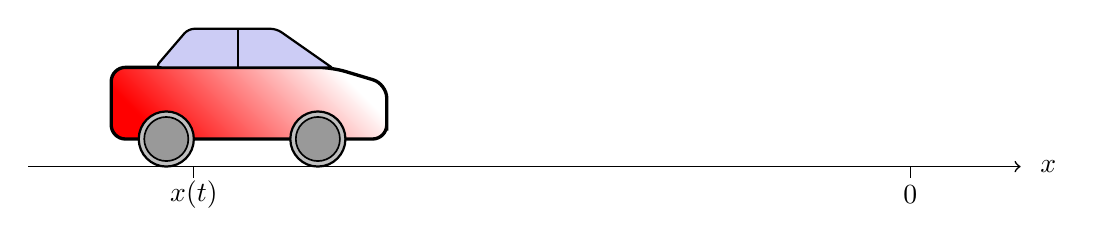
\begin{tikzpicture}[x=-0.7cm,y=0.7cm]
    \shade[top color=red, bottom color=white, shading angle={135}]
        [draw=black,fill=red!20,rounded corners=1.2ex,very thick] (1.5,.5) -- ++(0,1) -- ++(1,0.3) --  ++(3,0) -- ++(1,0) -- ++(0,-1.3) -- (1.5,.5) -- cycle;
    \draw[very thick, rounded corners=0.5ex,fill=black!20!blue!20!white,thick]  (2.5,1.8) -- ++(1,0.7) -- ++(1.6,0) -- ++(0.6,-0.7) -- (2.5,1.8);
    \draw[thick]  (4.2,1.8) -- (4.2,2.5);
    \draw[draw=black,fill=gray!50,thick] (2.75,.5) circle (.5);
    \draw[draw=black,fill=gray!50,thick] (5.5,.5) circle (.5);
    \draw[draw=black,fill=gray!80,semithick] (2.75,.5) circle (.4);
    \draw[draw=black,fill=gray!80,semithick] (5.5,.5) circle (.4);

    \draw[<-,semithick] (-10,0) -- (8,0);
    \draw (-10.5,0) node {$x$};
    \draw (5,0) -- (5,-.2);
    \draw (5,-.5) node {$x(t)$};
    \draw (-8,0) -- (-8,-.2);
    \draw (-8,-.5) node {$0$};
\end{tikzpicture}
\end{center}

Pour cela il envoie un signal $s(t)$.

\begin{questions}
    \questioncours Propagation unidimensionnelle d'une onde progressive. Cas des ondes électromagnétiques dans le vide. Déterminer $s(x,t)$.
    \uplevel{\`A l'instant $t = 0$, l'émetteur envoie un train d'ondes puis un second à
l'instant $t = T$, où $T$ est donc la période d'émission des trains d'ondes. Le signal se réfléchit ensuite sur le véhicule et revient vers le }
    \question Exprimer la période $T'$ perçue par le véhicule.
    \question De même exprimer la période $T''$ perçue par le récepteur du radar et montrer que
    $$f'' = \dfrac{1 + v/c}{1 - v/c}f \stackrel{v \ll c}{\simeq} 1 + 2\dfrac{v}{c}.$$
    \question Le radar envoie un signal sinusoidal de fréquence $f = \SI{24.125}{GHz}$. Interpréter le signal reçu :
\begin{EnvUplevel}
    \centering
    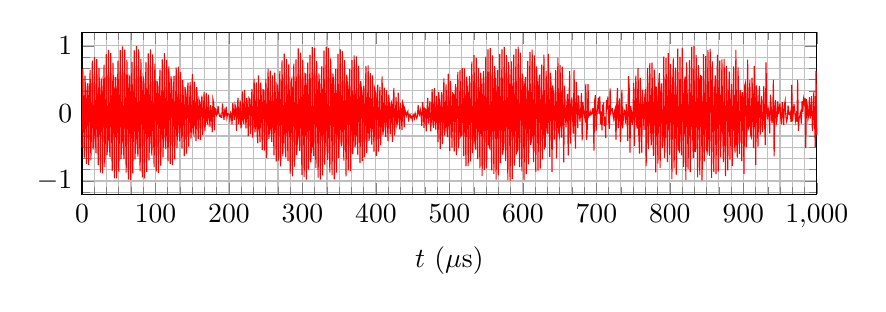
\begin{tikzpicture}
    \begin{axis}[
     clip=false,
     xmin=0,xmax=1000,
     xlabel= $t$ ($\mu$s),
     %axis lines=left,
     %axis x line=middle,
     %axis y line=left,
     width=.9\linewidth,
     height=.3\linewidth,
     ytick={},
     grid=both,
     minor tick num=5,
     ]
      \addplot[domain=0:1000,samples=1000,red]{0.5*sin(deg(x)*1e3)+0.5*sin(deg(x+.3)*(1e3+1.6e-7*24.125*1e3*2*pi))};
      %\addplot[domain=0:1000,samples=200,black,dashed]{cos(deg(x)*1.6e-7*24.125*1e3*pi)};
      %\addplot[domain=0:1000,samples=200,black,dashed]{-cos(deg(x)*1.6e-7*24.125*1e3*pi)};
    \end{axis}
  \end{tikzpicture}
\end{EnvUplevel}
Le véhicule respecte-t-il la limitation en vigueur ?
\uplevel{Pour que le signal soit plus exploitable, on effectue une détection synchrone : le signal reçu $s(t)$ est multiplié par le signal émis $s_0(t)$ et on lui applique un filtre qui coupe les fréquences plus grandes ou égales à $f$.}
    \question Quel est alors ce nouveau signal $g(t)$ ? En quoi ce nouveau signal est plus simple ?
\end{questions}
  

\end{exercise}

\begin{solution}
\begin{questions}
    \question Propagation : $s(x,t) = s(x - ct)$ à droite et $s(x,t) = s(x+ct)$ à gauche.
    \question $T' = \dfrac{1}{1+v/c}T$.
    \question $T'' = (1+v/c)T' = \dfrac{1-v/c}{1+v/c}T$.
    \question 88 km/h
    \question Montage 258
\end{questions}
\end{solution}
% Niveau :      PCSI
% Discipline :  Ondes signaux
% Mots clés :   Propagation des ondes

\begin{exercise}{Sono pourrie}{2}{Sup,Spé}
{Ondes,Propagation des ondes,Doppler}{bermudez}

\noindent\textsfbf{Problème ouvert}

Lors d'un concert de Ariana Grande à Bercy, vous avez le malheur de vous trouver au rang ZC à 150 m de la scène. La salle est approximativement de dimensions $\mathrm{150\,m\times 350\,m \times 30\,m}$. Les haut parleurs émettent la musique de part et d'autre de la scène, qui fait 30 mètres de long.

En quoi cette configuration risque d'altérer votre expérience de spectateur ?

\end{exercise}

\begin{solution}

On superpose deux signaux, modélisés comme sinusoidaux mais légèrement déphasés à cause d'une différence de propagation.

Soit la différence entre les deux haut-parleurs. Soit la différence entre le son direct et le son réfléchi sur le plafond. On peut regarder la différence entre les oreilles aussi.

On pourra étudier le temps d'écho également.
\end{solution}
%% RC passe bas
\begin{exercise}{Filtres linéaires du premier ordre}{0}{Sup}
{\'Electrocinétique,Filtrage linéaire, Premier ordre}{bermudez}

\begin{minipage}[t]{.3\linewidth}
\vspace{-1.5em}
\begin{circuitikz}
      \draw
      (0,0) to [open, v^=$\underline{e}$, *-o] (0,2)
      (0,2) to [R, l=$R$] (2,2) 
      to [C, l^=$C$, *-*] (2,0)
      (2,2) to [short] (3,2)
      (3,0) to [open, v_=$\underline{s}$, *-o] (3,2)
      (0,0) to [short] (3,0);
\end{circuitikz}
\vspace{1em}
\end{minipage}\begin{minipage}[t]{.7\linewidth}
    \textsf{Question de cours : } Déterminez la nature et le diagramme de Bode de ce filtre, en précisant sa fréquence de coupure et son gain statique.
\end{minipage}
\end{exercise}


% RL passe haut
\begin{exercise}{Filtres linéaires du premier ordre}{0}{Sup}
{\'Electrocinétique,Filtrage linéaire, Premier ordre}{bermudez}

\begin{minipage}[t]{.3\linewidth}
\vspace{-1.5em}
\begin{circuitikz}
      \draw
      (0,0) to [open, v^=$\underline{e}$, *-o] (0,2)
      (0,2) to [R, l=$R$] (2,2) 
      to [L, l^=$L$, *-*] (2,0)
      (2,2) to [short] (3,2)
      (3,0) to [open, v_=$\underline{s}$, *-o] (3,2)
      (0,0) to [short] (3,0);
\end{circuitikz}
\vspace{1em}
\end{minipage}\begin{minipage}[t]{.7\linewidth}
    \textsf{Question de cours : } Déterminez la nature et le diagramme de Bode de ce filtre, en précisant sa fréquence de coupure et son gain statique.
\end{minipage}
\end{exercise}


% RC passe bas
\begin{exercise}{Filtres linéaires du premier ordre}{0}{Sup}
{\'Electrocinétique,Filtrage linéaire, Premier ordre}{bermudez}

\begin{minipage}[t]{.3\linewidth}
\vspace{-1.5em}
\begin{circuitikz}
      \draw
      (0,0) to [open, v^=$\underline{e}$, *-o] (0,2)
      (0,2) to [C, l=$C$] (2,2) 
      to [R, l^=$R$, *-*] (2,0)
      (2,2) to [short] (3,2)
      (3,0) to [open, v_=$\underline{s}$, *-o] (3,2)
      (0,0) to [short] (3,0);
\end{circuitikz}
\vspace{1em}
\end{minipage}\begin{minipage}[t]{.7\linewidth}
    \textsf{Question de cours : } Déterminez la nature et le diagramme de Bode de ce filtre, en précisant sa fréquence de coupure et son gain statique.
\end{minipage}
\end{exercise}


% RL passe haut
\begin{exercise}{Filtres linéaires du premier ordre}{0}{Sup}
{\'Electrocinétique,Filtrage linéaire, Premier ordre}{bermudez}

\begin{minipage}[t]{.3\linewidth}
\vspace{-1.5em}
\begin{circuitikz}
      \draw
      (0,0) to [open, v^=$\underline{e}$, *-o] (0,2)
      (0,2) to [L, l=$L$] (2,2) 
      to [R, l^=$R$, *-*] (2,0)
      (2,2) to [short] (3,2)
      (3,0) to [open, v_=$\underline{s}$, *-o] (3,2)
      (0,0) to [short] (3,0);
\end{circuitikz}
\vspace{1em}
\end{minipage}\begin{minipage}[t]{.7\linewidth}
    \textsf{Question de cours : } Déterminez la nature et le diagramme de Bode de ce filtre, en précisant sa fréquence de coupure et son gain statique.
\end{minipage}
\end{exercise}


% Tableau des solutions

{
\def\thesolution{Solutions \arabicAlph{part}\arabicAlph{section}\hspace{2pt}01--\twodigits{exercise}\quad---\quad}
\begin{solution}

\newcounter{subsol}
\newcommand{\parti}{\large\bfseries\sffamily\stepcounter{subsol}\arabicAlph{part}\arabicAlph{section}\hspace{2pt}\twodigits{subsol}\quad}

\noindent\begin{tabularx}{\linewidth}{@{\parti}C@{\vspace{1em}}Ccp{5em}}

\begin{circuitikz}[baseline={(0,2)}]
      \draw
      (0,0) to [open, v^=$\underline{e}$, *-o] (0,2)
      (0,2) to [R, l=$R$] (2,2) 
      to [C, l^=$C$, *-*] (2,0)
      (2,2) to [short] (3,2)
      (3,0) to [open, v_=$\underline{s}$, *-o] (3,2)
      (0,0) to [short] (3,0);
\end{circuitikz} &
$ \underline{H}(\omega) = \dfrac{1}{1+j RC\omega}$ &
Passe-bas &
$H_0 = 1$, \newline $\omega_\text{c} = \dfrac{1}{RC}$ \\

\begin{circuitikz}[baseline={(0,2)}]
      \draw
      (0,0) to [open, v^=$\underline{e}$, *-o] (0,2)
      (0,2) to [R, l=$R$] (2,2) 
      to [L, l^=$L$, *-*] (2,0)
      (2,2) to [short] (3,2)
      (3,0) to [open, v_=$\underline{s}$, *-o] (3,2)
      (0,0) to [short] (3,0);
\end{circuitikz} &
$ \underline{H}(\omega) = \dfrac{j L/R\omega}{1+j L/R\omega}$ &
Passe-haut &
$H_0 = 1$, \newline $\omega_\text{c} = \dfrac{R}{L}$ \\

\begin{circuitikz}[baseline={(0,2)}]
      \draw
      (0,0) to [open, v^=$\underline{e}$, *-o] (0,2)
      (0,2) to [C, l=$C$] (2,2) 
      to [R, l^=$R$, *-*] (2,0)
      (2,2) to [short] (3,2)
      (3,0) to [open, v_=$\underline{s}$, *-o] (3,2)
      (0,0) to [short] (3,0);
\end{circuitikz} &
$ \underline{H}(\omega) = \dfrac{jRC\omega}{1+j RC\omega}$ &
Passe-haut &
$H_0 = 1$, \newline $\omega_\text{c} = \dfrac{1}{RC}$ \\

\begin{circuitikz}[baseline={(0,2)}]
      \draw
      (0,0) to [open, v^=$\underline{e}$, *-o] (0,2)
      (0,2) to [L, l=$L$] (2,2) 
      to [R, l^=$R$, *-*] (2,0)
      (2,2) to [short] (3,2)
      (3,0) to [open, v_=$\underline{s}$, *-o] (3,2)
      (0,0) to [short] (3,0);
\end{circuitikz} &
$ \underline{H}(\omega) = \dfrac{1}{1+j L/R\omega}$ &
Passe-bas &
$H_0 = 1$, \newline $\omega_\text{c} = \dfrac{R}{L}$ \\

\end{tabularx}

\end{solution}

}
 % AJOUTE
%% RLC passe bas 
\begin{exercise}{RLC série}{0}{Sup}
{\'Electrocinétique,Filtrage linéaire, Second ordre}{bermudez}

\begin{minipage}[t]{.4\linewidth}
\vspace{-1.5em}
\begin{circuitikz}
      \draw
      (0,0) to [open, v^=$\underline{e}$, *-o] (0,2)
      (0,2) to [R, l=$R$] (2,2)
      to [L, l=$L$] (4,2) 
      to [C, l^=$C$, *-*] (4,0)
      (4,2) to [short] (5,2)
      (5,0) to [open, v_=$\underline{s}$, *-o] (5,2)
      (0,0) to [short] (5,0);
\end{circuitikz}
\vspace{1em}
\end{minipage}\begin{minipage}[t]{.6\linewidth}
    \textsf{Question de cours : } Déterminez la nature et le diagramme de Bode de ce filtre, en précisant sa fréquence propre, sa fréquence de de résonance, son gain statique / à la résonance, et son facteur de qualité.
\end{minipage}
\end{exercise}



% RLC passe bande 
\begin{exercise}{RLC série}{0}{Sup}
{\'Electrocinétique,Filtrage linéaire, Second ordre}{bermudez}

\begin{minipage}[t]{.4\linewidth}
\vspace{-1.5em}
\begin{circuitikz}
      \draw
      (0,0) to [open, v^=$\underline{e}$, *-o] (0,2)
      (0,2) to [L, l=$L$] (2,2)
      to [C, l=$C$] (4,2) 
      to [R, l^=$R$, *-*] (4,0)
      (4,2) to [short] (5,2)
      (5,0) to [open, v_=$\underline{s}$, *-o] (5,2)
      (0,0) to [short] (5,0);
\end{circuitikz}
\vspace{1em}
\end{minipage}\begin{minipage}[t]{.6\linewidth}
    \textsf{Question de cours : } Déterminez la nature et le diagramme de Bode de ce filtre, en précisant sa fréquence propre, sa fréquence de de résonance, son gain statique / à la résonance, et son facteur de qualité.
\end{minipage}
\end{exercise}



% RLC passe haut 
\begin{exercise}{RLC série}{0}{Sup}
{\'Electrocinétique,Filtrage linéaire, Second ordre}{bermudez}

\begin{minipage}[t]{.4\linewidth}
\vspace{-1.5em}
\begin{circuitikz}
      \draw
      (0,0) to [open, v^=$\underline{e}$, *-o] (0,2)
      (0,2) to [R, l=$R$] (2,2)
      to [C, l=$C$] (4,2) 
      to [L, l^=$L$, *-*] (4,0)
      (4,2) to [short] (5,2)
      (5,0) to [open, v_=$\underline{s}$, *-o] (5,2)
      (0,0) to [short] (5,0);
\end{circuitikz}
\vspace{1em}
\end{minipage}\begin{minipage}[t]{.6\linewidth}
    \textsf{Question de cours : } Déterminez la nature et le diagramme de Bode de ce filtre, en précisant sa fréquence propre, sa fréquence de de résonance, son gain statique / à la résonance, et son facteur de qualité.
\end{minipage}
\end{exercise}




% Tableau des solutions

{
\def\thesolution{Solutions \arabicAlph{part}\arabicAlph{section}\hspace{2pt}01--\twodigits{exercise}\quad---\quad}
\begin{solution}
\ifx\thesubsol\undefined
    \newcounter{subsol}
 \else
    \setcounter{subsol}{-1}
 \fi
\def\parti{\large\bfseries\sffamily\stepcounter{subsol}\arabicAlph{part}\arabicAlph{section}\hspace{2pt}\twodigits{subsol}\quad}

\noindent\begin{tabularx}{\linewidth}{@{\parti}C@{\vspace{1em}}Cp{11em}}

\begin{circuitikz}[baseline={(0,2)}]
      \draw
      (0,0) to [open, v^=$\underline{e}$, *-o] (0,2)
      (0,2) to [R, l=$R$] (2,2)
      to [L, l=$L$] (4,2) 
      to [C, l^=$C$, *-*] (4,0)
      (4,2) to [short] (5,2)
      (5,0) to [open, v_=$\underline{s}$, *-o] (5,2)
      (0,0) to [short] (5,0);
\end{circuitikz}  &
$ \underline{H}(\omega) = \dfrac{1}{1+j RC\omega - LC\omega^2}$ &
Passe-bas du 2\textsuperscript{nd} ordre \newline
$H_0 = 1$, \newline $\omega_\text{c} = \dfrac{1}{\sqrt{LC}}$ \newline $Q = \dfrac{1}{R}\sqrt{\dfrac{L}{C}}$ \\

\begin{circuitikz}[baseline={(0,2)}]
      \draw
      (0,0) to [open, v^=$\underline{e}$, *-o] (0,2)
      (0,2) to [L, l=$L$] (2,2)
      to [C, l=$C$] (4,2) 
      to [R, l^=$R$, *-*] (4,0)
      (4,2) to [short] (5,2)
      (5,0) to [open, v_=$\underline{s}$, *-o] (5,2)
      (0,0) to [short] (5,0);
\end{circuitikz}  &
$ \underline{H}(\omega) = \dfrac{jRC\omega}{1+j RC\omega - LC\omega^2}$ &
Passe-bande du 2\textsuperscript{nd} ordre \newline
$H_0 = 1$, \newline $\omega_\text{c} = \dfrac{1}{\sqrt{LC}}$ \newline $Q = \dfrac{1}{R}\sqrt{\dfrac{L}{C}}$ \\

\begin{circuitikz}[baseline={(0,2)}]
      \draw
      (0,0) to [open, v^=$\underline{e}$, *-o] (0,2)
      (0,2) to [R, l=$R$] (2,2)
      to [C, l=$C$] (4,2) 
      to [L, l^=$L$, *-*] (4,0)
      (4,2) to [short] (5,2)
      (5,0) to [open, v_=$\underline{s}$, *-o] (5,2)
      (0,0) to [short] (5,0);
\end{circuitikz}  &
$ \underline{H}(\omega) = \dfrac{-LC\omega^2}{1+j RC\omega - LC\omega^2}$ &
Passe-haut du 2\textsuperscript{nd} ordre \newline
$H_0 = 1$, \newline $\omega_\text{c} = \dfrac{1}{\sqrt{LC}}$ \newline $Q = \dfrac{1}{R}\sqrt{\dfrac{L}{C}}$ \\

\end{tabularx}

\end{solution}

}
 % AJOUTE
%% RLC passe bas 
\begin{exercise}{Filtres linéaires du second ordre}{0}{Sup}
{\'Electrocinétique,Filtrage linéaire, Second ordre}{bermudez}

\begin{minipage}[t]{.4\linewidth}
\vspace{-1.5em}
\begin{circuitikz}
      \draw
      (0,0) to [open, v^=$\underline{e}$, *-o] (0,2)
      (0,2) to [R, l=$R$] (2,2)
      to [L, l=$L$] (4,2) 
      to [C, l^=$C$, *-*] (4,0)
      (4,2) to [short] (5,2)
      (5,0) to [open, v_=$\underline{s}$, *-o] (5,2)
      (0,0) to [short] (5,0);
\end{circuitikz}
\vspace{1em}
\end{minipage}\begin{minipage}[t]{.6\linewidth}
    \textsf{Question de cours : } Déterminez la nature et le diagramme de Bode de ce filtre, en précisant sa fréquence propre, sa fréquence de de résonance, son gain statique / à la résonance, et son facteur de qualité.
\end{minipage}
\end{exercise}



% RLC passe bande 
\begin{exercise}{RLC série}{0}{Sup}
{\'Electrocinétique,Filtrage linéaire, Second ordre}{bermudez}

\begin{minipage}[t]{.4\linewidth}
\vspace{-1.5em}
\begin{circuitikz}
      \draw
      (0,0) to [open, v^=$\underline{e}$, *-o] (0,2)
      (0,2) to [L, l=$L$] (2,2)
      to [C, l=$C$] (4,2) 
      to [R, l^=$R$, *-*] (4,0)
      (4,2) to [short] (5,2)
      (5,0) to [open, v_=$\underline{s}$, *-o] (5,2)
      (0,0) to [short] (5,0);
\end{circuitikz}
\vspace{1em}
\end{minipage}\begin{minipage}[t]{.6\linewidth}
    \textsf{Question de cours : } Déterminez la nature et le diagramme de Bode de ce filtre, en précisant sa fréquence propre, sa fréquence de de résonance, son gain statique / à la résonance, et son facteur de qualité.
\end{minipage}
\end{exercise}



% RLC passe haut 
\begin{exercise}{RLC série}{0}{Sup}
{\'Electrocinétique,Filtrage linéaire, Second ordre}{bermudez}

\begin{minipage}[t]{.4\linewidth}
\vspace{-1.5em}
\begin{circuitikz}
      \draw
      (0,0) to [open, v^=$\underline{e}$, *-o] (0,2)
      (0,2) to [R, l=$R$] (2,2)
      to [C, l=$C$] (4,2) 
      to [L, l^=$L$, *-*] (4,0)
      (4,2) to [short] (5,2)
      (5,0) to [open, v_=$\underline{s}$, *-o] (5,2)
      (0,0) to [short] (5,0);
\end{circuitikz}
\vspace{1em}
\end{minipage}\begin{minipage}[t]{.6\linewidth}
    \textsf{Question de cours : } Déterminez la nature et le diagramme de Bode de ce filtre, en précisant sa fréquence propre, sa fréquence de de résonance, son gain statique / à la résonance, et son facteur de qualité.
\end{minipage}
\end{exercise}




% Tableau des solutions

{
\def\thesolution{Solutions \arabicAlph{part}\arabicAlph{section}\hspace{2pt}01--\twodigits{exercise}\quad---\quad}
\begin{solution}

\newcounter{subsol}
\newcommand{\parti}{\large\bfseries\sffamily\stepcounter{subsol}\arabicAlph{part}\arabicAlph{section}\hspace{2pt}\twodigits{subsol}\quad}

\noindent\begin{tabularx}{\linewidth}{@{\parti}C@{\vspace{1em}}Cp{11em}}

\begin{circuitikz}[baseline={(0,2)}]
      \draw
      (0,0) to [open, v^=$\underline{e}$, *-o] (0,2)
      (0,2) to [R, l=$R$] (2,2)
      to [L, l=$L$] (4,2) 
      to [C, l^=$C$, *-*] (4,0)
      (4,2) to [short] (5,2)
      (5,0) to [open, v_=$\underline{s}$, *-o] (5,2)
      (0,0) to [short] (5,0);
\end{circuitikz}  &
$ \underline{H}(\omega) = \dfrac{1}{1+j RC\omega - LC\omega^2}$ &
Passe-bas du 2\textsuperscript{nd} ordre \newline
$H_0 = 1$, \newline $\omega_\text{c} = \dfrac{1}{\sqrt{LC}}$ \newline $Q = \dfrac{1}{R}\sqrt{\dfrac{L}{C}}$ \\

\begin{circuitikz}[baseline={(0,2)}]
      \draw
      (0,0) to [open, v^=$\underline{e}$, *-o] (0,2)
      (0,2) to [L, l=$L$] (2,2)
      to [C, l=$C$] (4,2) 
      to [R, l^=$R$, *-*] (4,0)
      (4,2) to [short] (5,2)
      (5,0) to [open, v_=$\underline{s}$, *-o] (5,2)
      (0,0) to [short] (5,0);
\end{circuitikz}  &
$ \underline{H}(\omega) = \dfrac{jRC\omega}{1+j RC\omega - LC\omega^2}$ &
Passe-bande du 2\textsuperscript{nd} ordre \newline
$H_0 = 1$, \newline $\omega_\text{c} = \dfrac{1}{\sqrt{LC}}$ \newline $Q = \dfrac{1}{R}\sqrt{\dfrac{L}{C}}$ \\

\begin{circuitikz}[baseline={(0,2)}]
      \draw
      (0,0) to [open, v^=$\underline{e}$, *-o] (0,2)
      (0,2) to [R, l=$R$] (2,2)
      to [C, l=$C$] (4,2) 
      to [L, l^=$L$, *-*] (4,0)
      (4,2) to [short] (5,2)
      (5,0) to [open, v_=$\underline{s}$, *-o] (5,2)
      (0,0) to [short] (5,0);
\end{circuitikz}  &
$ \underline{H}(\omega) = \dfrac{-LC\omega^2}{1+j RC\omega - LC\omega^2}$ &
Passe-haut du 2\textsuperscript{nd} ordre \newline
$H_0 = 1$, \newline $\omega_\text{c} = \dfrac{1}{\sqrt{LC}}$ \newline $Q = \dfrac{1}{R}\sqrt{\dfrac{L}{C}}$ \\

\end{tabularx}

\end{solution}

}
 % AJOUTE
%% Niveau :      PCSI
% Discipline :  Elec
% Mots clés :   Elec, Ordre 1

\begin{exercise}{Bobine réelle}{1}{Sup}
{\'Electrocinétique, Circuits d'ordre 1}{lelay}

\begin{questions}
    \questioncours Donne la loi reliant la tension aux bornes d'une bobine au courant qui la traverse, sous forme différentielle et complexe. Unité et ordre de grandeur de l'inductance d'une bobine.
    \question La bobine "idéale" existe-t-elle dans la vraie vie ? Justifie qu'on représente une bobine "réelle" par une bobine idéale et un résistance $r$ en série. Comment doit être $r$ afin de se rapproche le plus possible de la bobine idéale ?
    \question On cherche maintenant à trouver l'inductance d'une certaine bobine, en prenant en compte sa résistance interne. On considère le circuit ci-dessous, où $R$ vaut 100 $\Omega$ :
    \begin{circuit}
          \draw
          (0,0) to [open, v_=$\underline{e}$, *-o] (0,2)
          (0,2) to [R, l=$r$] (2,2) 
                to [L, l=$L$] (4,2)
                to [R, l=$R$] (4,0)
          (4,2) to [short] (6,2)
          (6,0) to [open, v_=$\underline{s}$, *-o] (6,2)
          (0,0) to [short] (6,0);
    \end{circuit}
    Donner sa fonction de transfert $\underline{H} = \frac{\underline{s}}{\underline{e}}$
    \question Tracer l'allure du graphe de $\abs{\underline{H}}$ et $\arg(\underline{H})$ en fonction de $\frac{\omega}{\omega_0}$ où $\omega_0$ est une pulsation caractéristique du système que l'on précisera.
    \question Si on se place à très basse fréquence et que le signal d'entrée $\underline{e}$ a une amplitude de 6 V, le signal de sortie présente une amplitude de 5 V. En déduire la valeur de $r$.
    \question On constate qu'à $f = 2.4$ kHz, les deux signaux $\underline{s}$ et $\underline{e}$ sont en quadrature de phase. En déduire la valeur de l'inductance $L$.
\end{questions}
\end{exercise}


\begin{solution}


\begin{questions}
    \questioncours $U = L\dv{i}{t}$, $L\sim 10$ mH
    \question Impossible ideale, une bobine est faite de fil long donc au bout d'un moment on doit avoir de la résistance. idéale : résistance nul du fil, donc $r=0$.
    \question On a un diviseur de tension : 
    $$ \underline{s} = \frac{R}{R\,+\,r + jL\omega}\underline{e}$$
    soit sous forme canonique
    $$ H(\omega) = \frac{H_0}{1 + j\frac{\omega}{\omega_0}}$$
    avec $H_0 = R/(R+r)$ et $\omega_0 = (R+r)/L$
    \question On a un passe bas d'ordre 1, avec une phase qui va de 0 à $-\pi/2$
    \question À très basse fréquence on $H = H_0 = 5/6$ d'où $r = R/5 = 20$ $\Omega$
    \question quadrature de phase : on a $\omega = \omega_0$. On en déduit $L = (R+r)/(2\pi f)$ soit 8 mH.
\end{questions}

\end{solution}

%\begin{exercise}{Héliosphère solaire}{0}{Spé}
{Electromagnetisme, Magétostatique, Theoreme d'ampère, Plaque de courant}{bermudez}

\begin{questions}
    \questioncours Énoncé (succint) du théorème d'Ampère, version locale et intégrale. Comment passe-t-on de l'un à l'autre ?
    \uplevel{Le soleil possède des structures apparentées à de très fines couches de courant dans lesquelles sont dissipées l'énergie issue de la fusion nucléaire de l'étoile. On se propose de les modéliser par un plan en $z = 0$, infiniment fin, ayant un courant surfacique $\vec{j}_s = j_s \ve_x$.}
    \question Trouver l'expression du champ magnétique $\vec{B}$ engendré par le plan de courant.
    \question On considère maintenant la quantité $u = \dfrac{\vec{B}^2}{2\mu_0}$, qui a la dimension d'une énergie par unité de volume. Quelle est l'énergie engendrée par le plan de courant ?
\end{questions}

\end{exercise}


\begin{exercise}{Fil électrique}{0}{Spé}
{Electromagnetisme, Theoreme d'Ampère}{bermudez}

\begin{questions}
    \questioncours Énoncé (succint) du théorème d'Ampère, version locale et intégrale. Comment passe-t-on de l'un à l'autre ?
    \question On considère un cylindre de longueur infinie et de rayon $R$ parcouru par un courant $I$ uniformément réparti sur sa section. Trouver l'expression du champ magnétique $\vec{B}$ engendré par le fil, pour $r \leq R$ et $r \geq R$.
    \question On considère maintenant la quantité $u = \dfrac{\vec{B}^2}{2\mu_0}$, qui a la dimension d'une énergie par unité de volume. Quelle est l'énergie contenue dans un cylindre de rayon $r \leq R$ et de hauteur $H$ ? Même question pour $r \geq R$.
\end{questions}

\end{exercise}


\begin{exercise}{Bobine}{0}{Spé}
{Electromagnetisme, Theoreme d'Ampère}{bermudez}

\begin{questions}
    \questioncours Énoncé (succint) du théorème d'Ampère, version locale et intégrale. Comment passe-t-on de l'un à l'autre ?
    \uplevel{On considère un solénoïde modélisé comme un ensemble de boucles de courant de rayon $R$ parcourues d'un courant $I$ disposées sur un même axe de révolution avec une densité linéique $n_\ell$. On néglige les effets de bord.}
    \question Trouver l'expression du champ magnétique $\vec{B}$ engendré par le solénoïde, pour $r \leq R$ et $r \geq R$.
    
    \question Rappeler la définition de l'inductance $L$ en électronique en termes du champ magnétique $\vB$ et du courant $I$ et déduire de la question précédente l'inductance $L$ du solénoide. La calculer pour une bobine typique de TP $n_\ell = 10^4$ tours/m.
    \question On considère maintenant la quantité $u = \dfrac{\vec{B}^2}{2\mu_0}$, qui a la dimension d'une énergie par unité de volume. Quelle est l'énergie contenue dans un cylindre de rayon $r \leq R$ et de hauteur $H$ ? Même question pour $r \geq R$.
    \question Retrouver l'expression usuelle de l'énergie emmagasinée par une inductance.
\end{questions}

\paragraph{Données}

\begin{itemize}
    \item susceptibilité magnétique du vide $\mu_0 \simeq 4\pi \times 10^{-7}$ H$\cdot\text{m}^{-1}$.
\end{itemize}

\end{exercise}

\newpage

\begin{exercise}{Câble coaxial}{2}{Spé}
{Electromagnetisme, Theoreme d'Ampère}{bermudez}

\begin{questions}
    \questioncours Énoncé (succint) du théorème d'Ampère, version locale et intégrale. Comment passe-t-on de l'un à l'autre ?
    \uplevel{On considère un câble coaxial constitué de deux cylindres concentriques de longueur infinie et de rayons $R_1$ et $R_2 > R_1$. La région intérieure $r < R_1$, l'âme, est conductrice et est parcourue par un courant $I$ réparti uniformément sur sa section. La région $R_1 < r < R_2$, la gaine, est isolante et un courant $-I$ est réparti à sa surface en $r = R_2$.}
    \question  Trouver l'expression du champ magnétique $\vec{B}$ engendré par le courant $I$ dans la gaine, l'âme et à l'extérieur du câble coaxial.
    \question Rappeler la définition de l'inductance $L$ en électronique en termes du champ magnétique $\vB$ et du courant $I$ et déduire de la question précédente l'inductance de ligne $\Lambda$ (par unité de longueur du câble). La calculer pour un câble BNC usuel.
    \question On considère maintenant la quantité $u = \dfrac{\vec{B}^2}{2\mu_0}$, qui a la dimension d'une énergie par unité de volume. Quelle est l'énergie contenue dans  une longueur $H$ de câble coaxial ?
    \question Retrouver l'expression usuelle de l'énergie emmagasinée par une inductance.
\end{questions}

\paragraph{Données}

\begin{itemize}
    \item susceptibilité magnétique du vide $\mu_0 \simeq 4\pi \times 10^{-7}$ H$\cdot\text{m}^{-1}$.
\end{itemize}

\end{exercise}

\begin{solution}
    \begin{questions}
        \question ~
        \question Âme : $B(r) = \dfrac{\mu_0 I}{2\pi}\dfrac{r}{R_1^2}$, Gaine : $B(r) = \dfrac{\mu_0 I}{2\pi}\dfrac{1}{r}$, Extérieur : $B = 0$.
        \question $\cal{E}_\text{m} = \dfrac{\mu_0 I^2}{2\pi} L\qty(\dfrac{1}{4} + \ln\dfrac{R_2}{R_1})$
        \question D'où $\Lambda = \dfrac{\mu_0}{2\pi}\qty(\dfrac{1}{4} + \ln\dfrac{R_2}{R_1})$ \\
        AN : $R_1 = 2$ mm, $R_2 = 4$ mm, $\Lambda \sim 10^{-6}$ H$\cdot\text{m}^{-1}$.
    \end{questions}
\end{solution} %MODIFIE

%\begin{exercise}{Usine alimentée par un courant sinusoïdal}{1}{Sup}{\'Electrocinétique,Régime sinusoidal forcé}{correge}

\begin{questions}
    \questioncours Montrer le lien entre valeur efficace et amplitude pour un signal sinusoïdal.

    \uplevel{Une usine, alimentée sous la tension sinusoïdale de valeur efficace $U=\SI{220}{V}$ et de fréquence $f=\SI{50}{Hz}$, consomme une puissance moyenne $P=\SI{100}{kW}$; son facteur de puissance est $\cos \phi=0.8$.}
    
    \question Calculer l'intensité efficace $I$. \\ On pourra montrer que $P$ ne dépend que de $U$ et $I$ et $\cos\phi$, $\phi$ étant le déphasage entre $u(t)$ et $i(t)$.

    \uplevel{Souvent, les installations industrielles et domestriques ont un caractère inductif (\emph{i.e.} se comportent comme une inductance résistive), lié à la présence de fils et de bobinages (moteurs, transformateurs~\emph{etc.}).}

    \question Représenter qualitativement dans le plan complexe $\ubar{u}$ et $\ubar{i}$ en prenant comme référence la phase de $\ubar{u}$, ainsi que l'argument $\varphi$ de l'impédance équivalente $\ubar{Z}$ de l'usine.

    \question EDF facture à l'usine la puissance moyenne consommée $P$. Sachant que le réseau pour acheminer l'électricité possède une résistance $R_\textsc{edf}$, quelle puissance $P_\text{f}$ doit fournir EDF en fonction de $P$, $R_\textsc{edf}$ et $I$ ? Que doit valoir $\phi$ pour réduire la charge sur le réseau ?
    
    \uplevel{EDF met en parallèle avec l'usine un condensateur de capacité $C$ de sorte que le facteur de puissance $\cos\phi_\text{tot}$ de l'ensemble soit maximal.}

    \question Compléter la figure de la question 3 en y représentant les amplitudes complexes de $\ubar{i}_C$ et $\ubar{i}_\text{tot}$.

    \question Que doit valoir $C$ pour que le facteur de puissance $\cos\phi = 1$ ? Calculer en pourcentage l'économie réalisée par le fournisseur de l'énergie électrique, l'industriel consommant toujours la même puissance.
\end{questions}
\end{exercise}

\begin{solution}
    \begin{questions}
        \question La valeur efficace est telle que :
        $$U^2 = \ev{u(t)^2} = {u_0}^2 \ev{\cos^2(\omega t)} = \dfrac{1}{2}{u_0}^2 \ev{1 + \cos(2\omega t)} = \dfrac{{u_0}^2}{2}.$$
        D'où $U = u_0/\sqrt{2}$.

        \question $P = \ev{u(t) i(t)} = 2 UI\ev{\cos(\omega t)\cos(\omega t + \phi)} = UI\ev{\cos\phi + \cos(2\omega t + \phi)} = UI\cos\phi$.

        AN. : $I = 568$ A.

        \question $\ubar{u} = \ubar{Z}\, \ubar{i}$, donc $u_0 = Z_0 i_0 e^{j(\phi + \varphi)}$, ce qui indique que $\varphi = -\phi$, l'angle entre $(Ox)$ et $\ubar{i}$. Comme $\ubar{Z} = R + jL\omega$, $0 < \varphi < \pi/2$ et donc $0 > \phi > -\pi/2$, quart bas droite du plan complexe.

        Ainsi $\cos\phi \ll 1$ : on diminue la puissance consommée.

        \question $$P_\text{f} = R_\textsc{edf} I^2 + \abs{Z}\cos\phi I^2 = \dfrac{R_\textsc{edf} I^2 + \abs{Z}\cos\phi}{\cos^2\phi}\dfrac{P^2}{U^2}.$$
        Ainsi pour une même puissance, la charge sur réseau diverge quand $\cos\phi = 0$, EDF tente donc d'optimiser en prenant $\phi = 0$.

        \question $\ubar{i}_C = jC\omega \ubar{u}$ sera donc dans l'axe $Oy$.
        
        $\ubar{i}_\text{tot} = \ubar{i} + \ubar{i}_C = j\qty(C\omega - \dfrac{1}{Z_0}\sin\varphi) + \dfrac{1}{Z_0}\cos\varphi\ubar{u}$ sera entre les deux.

        Pour que $\phi_\text{tot} = 0$, il faut que $\text{Im }\ubar{i}_C = - \text{Im }\ubar{i}$ soit $I_C = I \sin\varphi$ ou encore $C\omega = \dfrac{1}{Z_0}\sin\varphi$.

        \question Ainsi $C = \dfrac{\sin\varphi}{Z_0\omega}$. L'industriel économise donc d'un facteur $\dfrac{1 - \cos\phi}{\cos\phi} = 25\%$.
        
    \end{questions}
\end{solution} % MODIFIE

%% Niveau :      Spé
% Discipline :  Méca
% Mots clés :   Chaine, caténaire

\begin{exercise}{Analogie RMN et pendule en rotation}{2}{Spé}
{Mécanique,Mécanique en référentiel non galiléen,Pendule}{bermu}

\begin{questions}
    \questioncours Forces d'inertie d'entraînement et de Coriolis.
\begin{EnvUplevel}
Considérons un pendule rigide de longueur $\ell$ et de masse $m$ fixé en $O$ dans un champ de pesanteur $\vg = -g\ve_z$. Le pendule se trouve dans un référentiel $\cal{R}'$ en rotation uniforme à la vitesse $\Omega$ autour de l'axe $\ve_z$. \\
On se placera dans un système de coordonnées sphériques $(r,\theta,\varphi)$ où $\theta\in\qty[0,\pi]$ est l'angle entre $Oz$ et l'axe du pendule.
\end{EnvUplevel}
    \question Chercher les positions d'équilibre du pendule $\theta_\text{eq}$, ainsi que leur stabilité. \\
    On ne fera intervenir que la fréquence propre du pendule $\omega_0$ et la fréquence de rotation $\Omega$.
    \question Tracer pour plusieurs valeurs pertinentes de $\Omega$ le profil d'énergie potentielle ainsi que les positions d'équilibre stables et instables. Interpréter les différentes zones de ce graphe.
    \uplevel{Nous allons maintenant étudier la dynamique locale du pendule proche des positions d'équilibre.}
    \question Pour chaque position d'équilibre $\theta_{\text{eq}, i}$, en substituant $\theta$ dans l'équation de la dynamique du pendule par
    $$\theta = \theta_{\text{eq}, i} + \varepsilon_i,$$
    montrer que pour de faibles variations $\varepsilon_i$ autour de la position d'équilibre, l'équation de la dynamique devient à l'ordre 1 en $\varepsilon_i$
    \begin{itemize}
        \item celle d'un oscillateur harmonique classique de pulsation $\omega_i$, si elle est stable,
        \item celle d'un système exponentiellement divergent avec taux de croissance $\sigma_i$, si elle est instable.
    \end{itemize}
    Interpréter physiquement ces deux résultats en discutant notamment des limites du modèle.
    Tracer $\theta_{\text{eq}, i}$, $\omega_i$ et $\sigma_i$ en fonction de $\Omega$ et interpréter.
\end{questions}
\paragraph{Questions facultatives (niveau PC) :}
\begin{questions}
    \question Rappeler ce qu'est la précession de Larmor et dresser une analogie avec le système précédent.
    \question Rappeler ce qu'est une transition de phase, ou changement d'état. \\
    En quoi peut-on dire que ce système effectue une transition de phase à la pulsation $\omega_c$ ?
\end{questions}

\end{exercise}% MODIFIE

%% Niveau :      Spé
% Discipline :  Méca
% Mots clés :   Chaine, caténaire

\begin{exercise}{Gravimétrie terrestre}{3}{Spé}
{Mécanique,Mécanique en référentiel non galiléen,Pesanteur,Gravité,Forces d'inertie}{bermu}

\begin{questions}
    \questioncours Caractère conservatif de la force d'inertie d’entraînement et champ de pesanteur dans un référentiel non galiléen. 
    
\begin{EnvUplevel}
On considère le référentiel terrestre qui se situe en surface de la Terre à la latitude $\lambda$.

\end{EnvUplevel}
    \question \textsf{Question ouverte :} le champ de pesanteur $g$ varie plus significativement si on se déplace de $h = \SI{1}{m}$ vers le nord, vers l'est, ou en altitude ? \`A quelle conditions peut-on estimer que $g$ est constant ?
\end{questions}
\paragraph{Notations :} 
On note $\Omega_\textsc{t}$ la pulsation associée à la rotation de la Terre, et $R_\textsc{t}$ son rayon.

\hspace{4.3em}
On note $\lambda$ la latitude qui est l'angle entre l'équateur et point le étudié ($\lambda = 49^\circ$ à Paris).
\end{exercise}

\begin{solution}
\begin{questions}
    \questioncours $$\vec{g} = \vec{g}_0 + \vec{a}_\text{ie} = -\dfrac{GM}{(R_\textsc{t}+z)^2}\vec{e}_z + \Omega^2_\textsc{t} R_\textsc{t} \cos\lambda \vec{e}_h = -\grad\qty(\dfrac{GM}{R_\textsc{t}+h} + \dfrac{1}{2}\Omega^2_\textsc{t} R_\textsc{t}^2 \cos\lambda^2),$$
$\vec{e}_z$ étant la verticale locale (depuis le centre de la Terre) et $\vec{e}_h$ le projeté orthogonal depuis l'axe de rotation de la Terre.
    \question
    \begin{itemize}
        \item \textsf{Variation selon $y$ :} nulle
        \item \textsf{Variation selon $z$ :}
        $$\delta g \simeq \delta\qty(-\dfrac{GM}{(R_\textsc{t}+h)^2}) = g_0 \dfrac{2 \delta z}{R_\textsc{t}} \qquad \dfrac{\delta  g}{g_0} \simeq \SI{3e-7}{}$$
        Raisonnable donc pour $\delta z \ll R_\textsc{t}$.
        \item \textsf{Variation selon $x$ :}
        $$\delta g \simeq \delta\qty(\Omega^2_\textsc{t} R_\textsc{t} \cos\lambda) = \Omega^2_\textsc{t} R_\textsc{t} \sin\lambda \delta\lambda = \Omega^2_\textsc{t} \sin\lambda \delta x \qquad \dfrac{\delta  g}{g_0} \simeq \SI{4e-10}{}$$
        Toujours raisonnable car $a_\text{ie}/g_0 \simeq \SI{5e-3}{}$ au max.
    \end{itemize}
\end{questions}
\end{solution}

% Niveau :      Spé
% Discipline :  Méca
% Mots clés :   Chaine, caténaire

\begin{exercise}{Expérience de Cassini}{3}{Spé}
{Mécanique,Mécanique en référentiel non galiléen,Chute libre,Déviation vers l'est}{bermu}

\begin{questions}
    \questioncours Caractère galiléen approché du référentiel terrestre. \\
    On appuiera la démonstration d'ordres de grandeur et on estimera la contribution des forces d'inertie dans un problème de dynamique terrestre.
    

\begin{EnvUplevel}
On se propose d'étudier l'expérience effectuée par Cassini en 1679 à l'observatoire de Paris sur les effets du caractère non galiléen du référentiel terrestre sur la chute libre d'un corps de masse $m$, supposé ponctuel, lâché sans vitesse dans un puits de profondeur $h$, et situé à la latitude $\lambda$.

On se placera dans le repère $(O,x,y,z)$ placé à la surface de la Terre, $Ox$ pointant vers le nord et $Oy$ vers l'ouest.

\end{EnvUplevel}
    \question Donner les équations de la dynamique de la particule, projetées sur chaque axe.
    \question Considérant que les effets non-galiléens son faibles, simplifier l'équation de sorte à ce qu'il n'y ait qu'un terme de force suivant chaque composante et résoudre l'équation.
    \question \`A l'observatoire de Paris (lattitude $\lambda = 49^\circ$), dans un puits de $h = \SI{158}{m}$ de profondeur,\linebreak Cassini a mesuré une déviation vers l'est de $y = 28$ mm vers l'est. Interpréter.
    \questionbonus Montrer également qu'on devrait observer une faible déviation vers le sud.
\end{questions}
\paragraph{Notations :} 
On note $\Omega_\textsc{t}$ la pulsation associée à la rotation de la Terre, et $R_\textsc{t}$ son rayon.

\hspace{4.3em}
On note $\lambda$ la latitude qui est l'angle entre l'équateur et point le étudié ($\lambda = 49^\circ$ à Paris).\end{exercise}

\begin{solution}
\begin{questions}
    \questioncours Dynamique inférieure à 24 heures.
    \question 
    $$\dv{\vv}{t} = -g\vec{e}_z - 2\vec{\Omega}_\textsc{t}\cross\vv = -g\mqty(0,0,1) - 2\Omega_\textsc{t} \mqty(\cos\lambda\\0\\-\sin\lambda)\cross\mqty(\dot{x}\\\dot{y}\\\dot{z}).$$

    $$\left\lbrace\begin{array}{l}
        \ddot{x} = 2\Omega_\textsc{t} \sin\lambda \dot{y}  \\
        \ddot{y} = 2\Omega_\textsc{t} (\sin\lambda \dot{x} + \cos\lambda \dot{z})  \\
        \ddot{z} = -g - 2\Omega_\textsc{t} \cos\lambda \dot{y}
    \end{array}\right.$$
    \question Or on a $\dot{x}$ et $\dot{y}$ négligeables, donc :
    $$\left\lbrace\begin{array}{l}
        \ddot{x} = 2\Omega_\textsc{t} \sin\lambda \dot{y}  \\
        \ddot{y} = 2\Omega_\textsc{t} \cos\lambda \dot{z}  \\
        \ddot{z} = -g
    \end{array}\right.$$
    d'où
    \begin{align*}
        \ddot{z} &= -g &
        \dot{z} &= -gt &
        z &= -\dfrac{1}{2}gt^2 \\
        \ddot{y} &= -2\Omega_\textsc{t} \cos\lambda g t &
        \dot{y} &= -\Omega_\textsc{t} \cos\lambda g t^2 &
        y &= - \dfrac{1}{3}\Omega_\textsc{t} \cos\lambda g t^3 \\
        \ddot{x} &= -2\Omega_\textsc{t}^2 \cos\lambda \sin\lambda g t^2 &
        \dot{x} &= -\dfrac{2}{3}\Omega_\textsc{t}^2 \cos\lambda \sin\lambda g t^3 &
        x &= -\dfrac{1}{6}\Omega_\textsc{t}^2 \cos\lambda \sin\lambda g t^4
    \end{align*}
    or $t = \sqrt{\dfrac{2h}{g}}$ d'où
    $$\left\lbrace\begin{array}{l}
        x =  -\dfrac{2}{3}\Omega_\textsc{t}^2 \cos\lambda \sin\lambda \dfrac{h^2}{g} \\
        y = - \dfrac{1}{3}\Omega_\textsc{t} \cos\lambda g \qty(\dfrac{2h}{g})^{3/2} \\
        z = - h
    \end{array}\right.$$
    \question On introduit une longueur typique :
    $$\ell = \dfrac{g}{\Omega_\textsc{t}^2} \simeq \SI{1,8e9}{m}$$
    $$\left\lbrace\begin{array}{l}
        x =  -\dfrac{2}{3} \cos\lambda \sin\lambda \dfrac{h^2}{\ell} \\
        y = - \dfrac{2\sqrt{2}}{3} \cos\lambda h \sqrt{\dfrac{h}{\ell}} \\
        z = - h
    \end{array}\right.$$
    On retrouve bien l'ODG.
    \question Pour $x$ on trouve une déviation vers le sud de $x = \SI{0,13}{um}$
\end{questions}
\end{solution} % MODIFIE

%\begin{exercise}{Sismographe}{2}{Sup}
{Mécanique,Oscillateur harmonique amorti,Ressort,Amortisseur,Oscillateur harmonique forcé}{bermudez,mines}

\begin{questions}
    \questioncours Analogie formelle entre le circuit RLC et le système masse--ressort--amortisseur en régime sinusoïdal forcé. \textsl{On fera un tableau comparant les différentes grandeurs typiques (résonance, facteur de qualité) de ces systèmes du second ordre.}
\end{questions}

\begin{multicols}{2}
    On considère un capteur d'amplitude constitué d'un support et d'une masse $m$ reliés par un ressort de raideur $k$ et de longueur à vide $\ell_0$, et un amortisseur de constante $h$, tout deux de masses négligeables.

    Le support est animé d'un mouvement de type sinusoïdal : $x_1 = b \cos\omega t$ par rapport au référentiel terrestre $(Oxy)$, supposé galiléen.

    \vspace{1cm}

    ~

\begin{figure}[H]
    \centering
    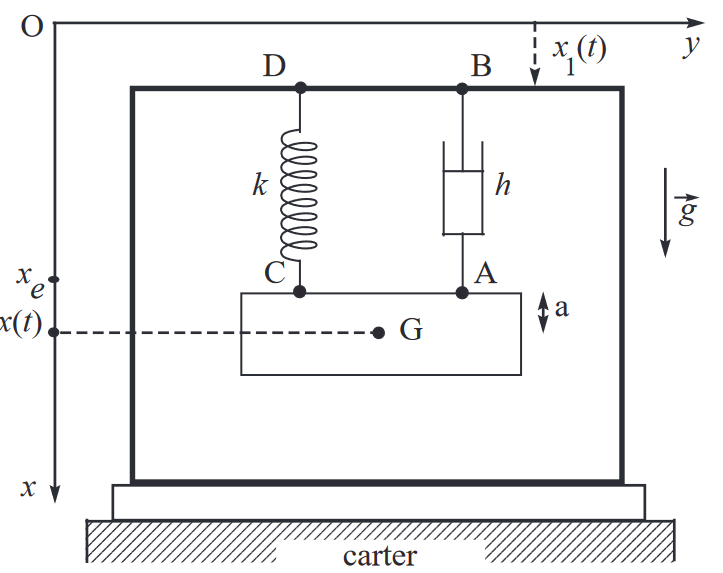
\includegraphics[width=\linewidth]{meca/oscharm/sismo.png}
    \caption{Schéma simplifié du sismomètre.}
\end{figure}
\end{multicols}

\begin{questions}    
\stepcounter{question}
    \question Déterminer l'expression de la position de la masse $m$ à l'équilibre $x_\text{eq}$ quand $x_1(t) = 0$ est immobile.
    \uplevel{On note $X(t) = x(t) - x_1(t) - x_\text{eq}$ la position relative d'une aiguille qui enregistre le signal dans le référentiel du support.}
    \question Déterminer l'équation du mouvement $x(t)$ de la masse $m$ dans le référentiel $(Oxy)$, puis dans la boite $X(t)$.
    \question Comment paramétrer $m$, $\gamma$ et $k$ pour avoir un bon sismomètre ?
\end{questions}
\end{exercise}

\begin{solution}
\begin{questions}
    \questioncours Les deux systèmes se mettent sous la forme :
    $$\ddot{X} + \dfrac{\omega_0}{Q}\dot{X} + \omega_0^2 X = F,$$
    avec : \\
    \begin{tabular}{c|c}
        \textbf{RLC série} & \textbf{Osc. méca} \\ \hline
        $X(t) = u_C(t)$ & $X(t) = x(t)$ \\
        $\omega_0 = \dfrac{1}{\sqrt{LC}}$ & $\omega_0 = \sqrt{\dfrac{k}{m}}$ \\
        $Q = \dfrac{1}{R}\sqrt{\dfrac{L}{C}}$ & $Q = \dfrac{1}{h}\sqrt{mk}$ \\ \hline
        $L$ & $m$ \\
        $C$ & $1/k$ \\
        $R$ & $h$
    \end{tabular}
    \question $x_e = \ell_0 + \dfrac{mg}{k} + a$
    \question PFD dans $(Oxy)$
    $$m\ddot{x} = - h\qty(\dot{x}(t) - \dot{x}_1(t)) - k\qty(x(t) - x_1(t) - x_\text{eq})$$
    ce qui donne
    $$\ddot{X} + \dfrac{\omega_0}{Q}\dot{X} + \omega_0^2 X = F,$$
    avec $F = b\omega^2$.
    \question L'amplitude de réaction est donc donnée par la fonction de transfert :
    $$H = \dfrac{X(t)}{x_1(t)} = \dfrac{1}{\sqrt{\qty(1-\dfrac{\omega_0^2}{\omega^2})^2 + \qty(\dfrac{\omega_0}{Q\omega})^2}}$$
    qui est un passe haut d'ordre 2.

    Ainsi pour limiter l'interie il faut $Q \leqslant 1$ et $\omega_0 \ll \omega_\text{typique séisme}$
\end{questions}
\end{solution}
 % NOUVEAU


%% Niveau :      PCSI *
% Discipline :  Méca
% Mots clés :   Ballistique, Mécanique du point, PFD, Chute libre

\begin{exercise}{Parabole de sureté}{2}{Sup, Spé}
{Mécanique,Mécanique du point}{bedo,bermu}

\begin{questions}
\questioncours Conservation de l'énergie mécanique. Cas d'une chute libre.

\uplevel{
On considère un point matériel $m$ en chute libre dans un champ de pesanteur $g$ partant initialement de $(0,0)$ avec une vitesse initiale $$\vv_0 = v_0\cos\theta\ve_x + v_0\sin\theta\ve_z.$$
}

\question Quelle est l'altitude maximale $H$ que $m$ peut atteindre ? Pour quel angle de tir $\theta$ cette altitude est-elle atteinte ?

\question Quelle est la trajectoire $z(x)$ de $m$ ? On exprimera $z$ uniquement en fonction de $x$, $\tan\theta$ et $H$.\\[-2em]
\uplevel{\textbf{\sffamily Indication :} $\dfrac{1}{\cos^2 x} = 1 + \tan^2 x$.

\bigskip

Par la suite, on chercher à tirer sur une cible $M$ de coordonnées $(X,Z)$ avec la balle $m$.

On appelle \emph{parabole de sûreté} la courbe qui enveloppe toutes les trajectoires possibles de $m$, la norme de sa vitesse initiale $v_0$ étant constante.}

\question Déduire de la question précédente l'équation de la parabole de sûreté de ce tir balistique.

\question Qu’en est-il lorsque l’on prend en compte les frottements de l’air ? Donner qualitativement le changement des résultats précédents.
\end{questions}
\end{exercise}

\begin{solution}
\begin{questions}
    \questioncours $\vec{F} = m\vec{a}$
    \question Par intégration : $\vr(t) = -\dfrac{1}{2}\vg t^2 + \vv_0 t$, d'où la parabole
    $$z = -\dfrac{g}{2 {v_0}^2}(1 + \tan^2\theta)x^2 + \tan\theta x.$$
    \question Une considération d'énergie mécanique permet d'obtenir que : $m g h = \dfrac{1}{2}m v_0^2$. L'altitude maximale est donc $h = \dfrac{{v_0}^2}{2g}$, pour $\theta = 0$.
    \question 
    $$z = -\dfrac{1}{4 h}(1 + \tan^2\theta)x^2 + \tan\theta x.$$
     \questionIl faut que
    $$z_0 = -\dfrac{1}{4 h}(1 + \tan^2\theta){x_0}^2 + \tan\theta x_0.$$
    Donc le discriminant par rapport à $\tan\theta$ doit être positif ou nul
    $$h - z_0 - \dfrac{{x_0}^2}{4 h} \geqslant 0.$$
   \questionPour le cas limite on trouve l'équation de la parabole de sûreté
    $$z = h - \dfrac{x^2}{4 h},$$
    telle que si $(x_0,z_0)$ est à l'intérieur, il est touché.
    \question Qualitativement, la parabole de sûreté est plus petite (le projectile va moins haut moins loin), il faut viser plus haut pour aller un peu plus loin (a priori le projectile sera aussi ralenti verticalement dans sa chute que la balle).
\end{questions}
\end{solution}

%\section{Parabole de s\^uret\'e}
%\tags{M\'ecanique du point} \\
%\level{Sup} \\
%\difficulty{1}

%On cherche à tirer un projectile avec une vitesse $V_0$ sur un point $M$. Le but de l'exercice est de trouver un critère simple pour savoir si cela est ou non possible.
%\begin{questions}
%\question \'Ecrire l'\'equation cartésienne $z(x)$ de la parabole décrite par le projectile
%\question Le point $M$ est-il toujours solution de cette équation ?
%\question En déduire l'équation de la parabole de sûreté d'un tir balistique
%\end{questions}

%\section{Tir au pigeon}
%\tags{M\'ecanique du point} \\
%\level{Sup} \\
%\difficulty{2}

%À $t=0$, on tire avec un canon orienté avec un angle $\theta$ sur un objet lâché en chute libre.
%\begin{questions}
%\question On suppose dans un premier temps qu'il n'y a pas de frottements.
%    \begin{parts}
%        \part À quel temps $t$ le projectile atteindra-t-il l'abscisse de la cible ?
%        \part En déduire $\theta$. La puissance du canon est-elle importante ?
%    \end{parts}
%\question On suppose maintenant que le problème prend en compte les frottements.
%    \begin{parts}
%        \part Quels changements attend-t-on par rapport à la situation précédente ?
%        \part Proposer une modélisation des frottements.
%        \part Dans quel cas la situation précédente est-elle toujours vérifiée ?
%    \end{parts}
%\end{questions}

\begin{exercise}{Il touche à tous les coups}{2}{Sup, Spé}
{Mécanique,Mécanique du point}{bedo,bermu}

\begin{questions}
\questioncours Principe fondamental de la dynamique

\uplevel{
On considère un point matériel $P$ en chute libre dans un champ de pesanteur $g$ partant initialement de $(x_0,z_0,0)$ sans vitesse. On cherche à tirer dessus avec une balle $M$ partant de $(0,0)$ avec une vitesse $$\vv_0 = v_0\cos\theta\ve_x + v_0\sin\theta\ve_z.$$
}

\question Quelle est la trajectoire $X(t)$ et $Z(t)$ du point $P$ ?

\question Quelle est la trajectoire $x(t)$ et $z(t)$ de la balle $M$ ?

\question À quel temps $t$ la balle atteindra sa cible ?

\question En déduire la direction $\theta$ qu'il faut viser initialement pour qu’un tir balistique atteigne sa cible si elle est également en chute libre ? En quoi la puissance du canon intervient-elle ? Interpréter ces résultats.
\end{questions}
\end{exercise} % MODIFIE

% \section{\'Electrostatique}
% \begin{exercise}{Condensateur plan}{1}{Spé}
{Electromagnetisme, Theoreme de gauss}{lelay,bermudez}

\paragraph{Point méthode en électromagnétisme :}
\begin{itemize}
    \item à partir de la géométrie de problème, choisir le bon système de coordonnées ;
    \item utiliser les invariances du problème pour réduire le nombre de variables ;
    \item utiliser les symétries pour réduire le nombre de composantes ;
    \item identifier une surface fermée, un contour \emph{etc.} et appliquer le théorème intégral pertinent.
\end{itemize}

\begin{questions}
    \questioncours Énoncé du théorème de Gauss. \\
    Donner sa version locale. Comment passe-t-on de l'un à l'autre ?
    \uplevel{On considère un plan infini dans le vide, en $z=0$, uniformément chargé par une charge surfacique~$\sigma$.}
    \question Donner l'expression du champ électrique $\vec{E}$ engendré par le plan chargé, en veillant bien à distinguer plusieurs cas.
    \uplevel{On considère maintenant deux plans infinis et parallèles, l'un de charge surfacique $\sigma$ placé en $z = -d/2$ et l'autre de charge surfacique $-\sigma$ placé en $z = d/2$.}
    \question Quel est le champ électrique résultant hors des deux plans ($\abs{z} > d/2$) ? Quel est le champ électrique entre les deux plans ($\abs{z} < d/2$) ?
    \question Quel est le potentiel électrique $V(z)$ à l'intérieur et à l'extérieur du condensateur.
    \question On appelle $U$ la différence de potentiel entre les deux plans. Exprimer $U$ en fonction de $\sigma$, $d$ et $\epsilon_0$.
    \question Dans un condensateur électrique, quelle est le lien entre sa charge $q$, la différence de potentiel $U$ sa capacité $C$ ? En déduire le lien entre $C$ et les caractéristiques géométriques du condensateur (sa surface $S$, nottament). 
    \uplevel{En réalité, le milieu entre les deux armatures n'est pas le vide mais un diéléctrique (il faut donc remplacer $\ep_0$ par $\ep_0\ep_r$).}
    \question \textsf{Application numérique :} condensateur céramique constitué d'armatures circulaires de diamètre 5 mm et d'une épaisseur de 1 $\mu$m de céramique de permittivité $\ep_r = 200$, $\ep_0 = \SI{8.9e-12}{F.m^{-1}}$.
								  
    %\questionbonus On suppose maintenant que l'espace entre les plaques la distribution suivante de charge volumique dans l'espace : $\rho(x, y, z \geq 0) = \rho_0 e^{-z/\lambda}$ où $\lambda$ est une constante, et $\rho(x, y, z<0) = 0$. Quel est le champ électrique $\vec{E}(x, y, z)$ pour $z < 0$ ? Pour $z \geq 0$ ?
\end{questions}

\end{exercise}


\begin{exercise}{Cylindre infini}{1}{Spé}
{Electromagnetisme, Theoreme de gauss}{lelay,bermudez}

\paragraph{Point méthode en électromagnétisme :}
\begin{itemize}
    \item à partir de la géométrie de problème, choisir le bon système de coordonnées ;
    \item utiliser les invariances du problème pour réduire le nombre de variables ;
    \item utiliser les symétries pour réduire le nombre de composantes ;
    \item identifier une surface fermée, un contour \emph{etc.} et appliquer le théorème intégral pertinent.
\end{itemize}

\begin{questions}
    \questioncours Énoncé du théorème de Gauss. \\
    Donner sa version locale. Comment passe-t-on de l'un à l'autre ?
    \uplevel{On considère un cylindre de rayon $R$ de longueur infinie dans le vide, uniformément chargé par une charge volumique $\rho$.}
    \question Donner l'expression du champ électrique $\vec{E}$ engendré par le cylindre chargé, en veillant bien à distinguer plusieurs cas.
    \question Donner l'expression du potentiel électrique $V(r)$ correspondant. Que se passe-t-il quand $r$ tend vers l'infini ? Est-ce physique ? Quelle hypothèse de départ cause ce problème ?
    %\question On considère maintenant la quantité $u = \frac12 \epsilon_0 \vec{E}^2$, qui a la dimension d'une énergie par unité de volume. Quelle est l'énergie contenue dans un cylindre de rayon $r \leq R$ et de hauteur $H$ ? Même question pour $r \geq R$.
								  
    %\question En remplaçant le cylindre infini par une sphère de rayon $R$, calculez l'énergie contenue dans une sphère de rayon $r \geq R$. Quelle est la limite de cette énergie lorsque $r$ tend vers l'infini ?
\end{questions}

\end{exercise}



\begin{exercise}{La Terre creuse}{1}{Spé}
{Electromagnetisme, Theoreme de gauss}{lelay,bermudez}

\paragraph{Point méthode en électromagnétisme :}
\begin{itemize}
    \item à partir de la géométrie de problème, choisir le bon système de coordonnées ;
    \item utiliser les invariances du problème pour réduire le nombre de variables ;
    \item utiliser les symétries pour réduire le nombre de composantes ;
    \item identifier une surface fermée, un contour \emph{etc.} et appliquer le théorème intégral pertinent.
\end{itemize}

\begin{questions}
    \questioncours Énoncé du théorème de Gauss. \\
    Donner sa version locale. Comment passe-t-on de l'un à l'autre ?
    \uplevel{On considère une sphère de rayon $R_1$ dans le vide, uniformément chargée par une charge volumique $\rho$.}
    \question Donner l'expression du champ électrique $\vec{E}_1$  engendré par la sphère chargée, en veillant bien à distinguer plusieurs cas.
    \question On considère maintenant une autre sphère dans le vide de charge $-\rho$ et de rayon $R_2 < R_1$. Quel est le champ $\vec{E}_2$ généré par cette seconde sphère ?
    \question En déduire le champ engendré une sphère creuse, uniformément chargée par une densité volumique de charge $\rho$ comprise entre les rayons interne $R_2$ et externe $R_1$.
	 
		  
		  
		  
	  
    \question Que penser des théories de la Terre creuse selon lesquelles la Terre est en fait creuse et qu'une partie de l'humanité pourrait habiter à l'intérieur ?
    %\question On considère maintenant une sphère de rayon $R$ et de charge $Q$ et on introduit la quantité $u = \frac12 \epsilon_0 \vec{E}^2$, qui a la dimension d'une énergie par unité de volume. Quelle est l'énergie contenue dans une sphère de rayon $r \leq R$ ? $r \geq R$ ? Dans tout l'espace ?
\end{questions}

\end{exercise}

% % Niveau :      PC
% Discipline :  Electromagnétisme
%Mots clés :    Equations de Maxwell, Debye-Hückel

\begin{exercise}{Cerceau -- Dipole}{3}{Spé}
{\'Electromagnétisme,\'Electrostatique,Statique des fluides}{bermu}

\begin{questions}
    \questioncours Quelle est l'expression du potentiel $V(\vr)$ et du champ $\vE(\vr)$ électriques de deux charges ponctuelles de signes opposés $\pm q$ distantes de $d$. \\
    Sans calcul, comment généraliser cela à une distribution continue ?
\begin{EnvUplevel}

On considère une distribution linéaire de charge électrique de forme circulaire, de rayon $R$ et de charge totale $q$. On appelle $O$ le centre du cercle. 

On définit $Oz = (O, \ve_z)$ l'axe de symétrie de la distribution. On étudiera uniquement les effets de la distribution pour une charge test située en $Oz$.
\end{EnvUplevel}
    \question Faire un schéma de la situation et introduire un système de coordonnées pertinent.
    \question Discuter les éléments de symétrie de la distribution et en déduire la forme attendue du champ $\vE(z)$ pour un observateur situé sur $Oz$.
    \question Calculer la contribution au potentiel électrique $\dd{V}(z)$ d'un élément $\dd{q}$ de la distribution --- qu'on exprimera dans le système de coordonnées choisi --- pour un observateur situé en $z$ sur $Oz$.
    \question En déduire le potentiel total $V(z)$ généré par le cercle en $z$, puis le champ électrique $\vE(z)$.
    \question Soit une charge test $q'$ contrainte sur l'axe $Oz$. Etablir la dynamique de $q'$ proche de $z = 0$.
\uplevel{On considère que cette charge $q' = -q$ est désormais fixée en $z = d$.}
    \question Quel est le potentiel total $V'$ ressenti pour un observateur en $z$ ?
    \question Montrez que la distribution totale se comporte comme un dipôle, dont on calculera le moment dipolaire $\vec{p}$.
    \question Quid du cas $d = 0$ ?
\end{questions}


\end{exercise}

\begin{solution}
\begin{questions}
    \questioncours 
    \question
    \question
    \question $\dd{V} = \dfrac{q\dd{\theta}/2\pi}{4\pi\varepsilon_0 \sqrt{R^2 + z^2}}$
    \question $V = \dfrac{q}{4\pi\varepsilon_0 \sqrt{R^2 + z^2}}$, $\vE = \dfrac{q z}{4\pi\varepsilon_0 (R^2 + z^2)^{3/2}}$
\end{questions}
\end{solution}
% % Niveau :      PC
% Discipline :  Electromagnétisme
%Mots clés :    Equations de Maxwell, Debye-Hückel

\begin{exercise}{Forces de Van der Waals}{3}{Spé}
{\'Electromagnétisme,\'Electrostatique,Statique des fluides}{bermu}

\begin{questions}
    \questioncours Quelle est l'expression du potentiel $V(\vr)$ et du champ $\vE(\vr)$ électriques de deux charges ponctuelles de signes opposés $\pm q$ distantes de $d$ ?
    \question Obtenir l'expression de la force et de l'énergie potentielle $\En_p$ exercée sur ce dipôle par un champ électrique extérieur $\vE_\text{ext}$.
    \question Rappeler le principe des forces de Van der Waals.
   
\begin{EnvUplevel}

On se place en deux dimensions. On considère deux molécules modélisées comme des dipôles permanents $\vp_1$ et $\vp_2$ fixées en $x = \pm d/2, y = 0$. On utilisera la notation
$$\kappa = \dfrac{p_1 p_2}{4\pi\varepsilon_0}.$$
\end{EnvUplevel}
    \question Donner l'énergie potentielle d'interaction des deux dipôles.
    \question \'Etablir les équations de la dynamique de $\vp_2$, $\vp_1$ étant constant.
    \question Donner la force appliquée à $\vp_1$ due à $\vp_2$.
    \question \`A l'aide des deux questions précédentes, donner la force moyenne subie par $\vp_1$ considéré comme fixe sachant que $\vp_2$ varie, étant soumis à la dynamique calculée à la question précédente.
\end{questions}


\end{exercise}

% \begin{exercise}{Foudre dans un pré}{2}{Spé}
{Electrostatique}{correge}

Un éclair frappe le sol au milieu d'un pré, à proximité d'une vache. Nous cherchons à savoir si cette vache est en sécurité. On modélise la foudre par un fil rectiligne vertical semi-infini, parcouru par un courant $I$. La vache se trouve à une distance $d$ du point d'impact, et la distance entre ses pattes est notée $p$. 

\begin{center}
    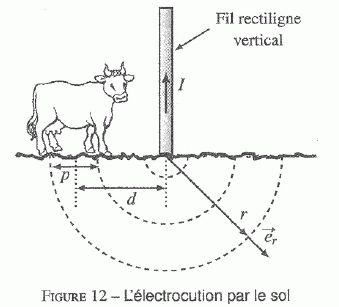
\includegraphics[width=0.4\linewidth]{electromag/electrostat/vache_foudre.png}
\end{center}

\begin{questions}

    \question Déterminer la densité de courant électrique $\vec{j}$ dans le sol.
    \question Rappeler l'expression de la loi d'ohm locale. Exprimer le champ électrique dans le sol et en déduire son potentiel $V(r)$ en le supposant nul à l'infini.
    \question Exprimer en fonction de $p$ et $d$ les potentiels au niveau des pattes avant et arrière de la vache. Quelle est la tension entre les pattes de la vache ?
    \question A quelle distance minimale $d_m$ du point d'impact est-elle en sécurité ?
    
    
    
\end{questions}

\paragraph{Données :} 
\begin{itemize}
    \item Foudre : $I=\SI{15}{kA}$
    \item Conductivité électrique du sol : $\gamma = \SI{1}{S/m}$
    \item Résistance de la vache : $R= \SI{30}{k\Omega}$
    \item Distance entre les pattes : $p=\SI{1.5}{m}$
    \item Courant létal pour une vache : $I_{max} = \SI{25}{mA}$
\end{itemize}

\end{exercise}

\begin{solution}
\begin{questions}

    \question $\vec j(r) = \frac{-I}{2\pi r^2} \vec{e}_r$
    \question $V(r) = \frac{-I}{2\pi \gamma  r} $
    \question $U = V(d+\frac{p}{2}) - V(d+\frac{p}{2}) \approx \frac{Ip}{2\pi \gamma d^2} $
    \question $d_m = \sqrt{\frac{Ip}{2\pi \gamma R I_{max} }}$
    
\end{questions}
\end{solution}


% \section{Magnétostatique}
% \begin{exercise}{Héliosphère solaire}{0}{Spé}
{Electromagnetisme, Magétostatique, Theoreme d'ampère, Plaque de courant}{bermudez}

\begin{questions}
    \questioncours Énoncé (succint) du théorème d'Ampère, version locale et intégrale. Comment passe-t-on de l'un à l'autre ?
    \uplevel{Le soleil possède des structures apparentées à de très fines couches de courant dans lesquelles sont dissipées l'énergie issue de la fusion nucléaire de l'étoile. On se propose de les modéliser par un plan en $z = 0$, infiniment fin, ayant un courant surfacique $\vec{j}_s = j_s \ve_x$.}
    \question Trouver l'expression du champ magnétique $\vec{B}$ engendré par le plan de courant.
    \question On considère maintenant la quantité $u = \dfrac{\vec{B}^2}{2\mu_0}$, qui a la dimension d'une énergie par unité de volume. Quelle est l'énergie engendrée par le plan de courant ?
\end{questions}

\end{exercise}


\begin{exercise}{Fil électrique}{0}{Spé}
{Electromagnetisme, Theoreme d'Ampère}{bermudez}

\begin{questions}
    \questioncours Énoncé (succint) du théorème d'Ampère, version locale et intégrale. Comment passe-t-on de l'un à l'autre ?
    \question On considère un cylindre de longueur infinie et de rayon $R$ parcouru par un courant $I$ uniformément réparti sur sa section. Trouver l'expression du champ magnétique $\vec{B}$ engendré par le fil, pour $r \leq R$ et $r \geq R$.
    \question On considère maintenant la quantité $u = \dfrac{\vec{B}^2}{2\mu_0}$, qui a la dimension d'une énergie par unité de volume. Quelle est l'énergie contenue dans un cylindre de rayon $r \leq R$ et de hauteur $H$ ? Même question pour $r \geq R$.
\end{questions}

\end{exercise}


\begin{exercise}{Bobine}{0}{Spé}
{Electromagnetisme, Theoreme d'Ampère}{bermudez}

\begin{questions}
    \questioncours Énoncé (succint) du théorème d'Ampère, version locale et intégrale. Comment passe-t-on de l'un à l'autre ?
    \uplevel{On considère un solénoïde modélisé comme un ensemble de boucles de courant de rayon $R$ parcourues d'un courant $I$ disposées sur un même axe de révolution avec une densité linéique $n_\ell$. On néglige les effets de bord.}
    \question Trouver l'expression du champ magnétique $\vec{B}$ engendré par le solénoïde, pour $r \leq R$ et $r \geq R$.
    
    \question Rappeler la définition de l'inductance $L$ en électronique en termes du champ magnétique $\vB$ et du courant $I$ et déduire de la question précédente l'inductance $L$ du solénoide. La calculer pour une bobine typique de TP $n_\ell = 10^4$ tours/m.
    \question On considère maintenant la quantité $u = \dfrac{\vec{B}^2}{2\mu_0}$, qui a la dimension d'une énergie par unité de volume. Quelle est l'énergie contenue dans un cylindre de rayon $r \leq R$ et de hauteur $H$ ? Même question pour $r \geq R$.
    \question Retrouver l'expression usuelle de l'énergie emmagasinée par une inductance.
\end{questions}

\paragraph{Données}

\begin{itemize}
    \item susceptibilité magnétique du vide $\mu_0 \simeq 4\pi \times 10^{-7}$ H$\cdot\text{m}^{-1}$.
\end{itemize}

\end{exercise}

\newpage

\begin{exercise}{Câble coaxial}{2}{Spé}
{Electromagnetisme, Theoreme d'Ampère}{bermudez}

\begin{questions}
    \questioncours Énoncé (succint) du théorème d'Ampère, version locale et intégrale. Comment passe-t-on de l'un à l'autre ?
    \uplevel{On considère un câble coaxial constitué de deux cylindres concentriques de longueur infinie et de rayons $R_1$ et $R_2 > R_1$. La région intérieure $r < R_1$, l'âme, est conductrice et est parcourue par un courant $I$ réparti uniformément sur sa section. La région $R_1 < r < R_2$, la gaine, est isolante et un courant $-I$ est réparti à sa surface en $r = R_2$.}
    \question  Trouver l'expression du champ magnétique $\vec{B}$ engendré par le courant $I$ dans la gaine, l'âme et à l'extérieur du câble coaxial.
    \question Rappeler la définition de l'inductance $L$ en électronique en termes du champ magnétique $\vB$ et du courant $I$ et déduire de la question précédente l'inductance de ligne $\Lambda$ (par unité de longueur du câble). La calculer pour un câble BNC usuel.
    \question On considère maintenant la quantité $u = \dfrac{\vec{B}^2}{2\mu_0}$, qui a la dimension d'une énergie par unité de volume. Quelle est l'énergie contenue dans  une longueur $H$ de câble coaxial ?
    \question Retrouver l'expression usuelle de l'énergie emmagasinée par une inductance.
\end{questions}

\paragraph{Données}

\begin{itemize}
    \item susceptibilité magnétique du vide $\mu_0 \simeq 4\pi \times 10^{-7}$ H$\cdot\text{m}^{-1}$.
\end{itemize}

\end{exercise}

\begin{solution}
    \begin{questions}
        \question ~
        \question Âme : $B(r) = \dfrac{\mu_0 I}{2\pi}\dfrac{r}{R_1^2}$, Gaine : $B(r) = \dfrac{\mu_0 I}{2\pi}\dfrac{1}{r}$, Extérieur : $B = 0$.
        \question $\cal{E}_\text{m} = \dfrac{\mu_0 I^2}{2\pi} L\qty(\dfrac{1}{4} + \ln\dfrac{R_2}{R_1})$
        \question D'où $\Lambda = \dfrac{\mu_0}{2\pi}\qty(\dfrac{1}{4} + \ln\dfrac{R_2}{R_1})$ \\
        AN : $R_1 = 2$ mm, $R_2 = 4$ mm, $\Lambda \sim 10^{-6}$ H$\cdot\text{m}^{-1}$.
    \end{questions}
\end{solution}
% \begin{exercise}{Piège de Ioffe--Pritchard}{2}{Spé}
{Magnétostatique}{bermu, lelay}

\paragraph{Point méthode en électromagnétisme :}
\begin{itemize}
    \item à partir de la géométrie de problème, choisir le bon système de coordonnées ;
    \item utiliser les invariances du problème pour réduire le nombre de variables ;
    \item utiliser les symétries pour réduire le nombre de composantes ;
    \item identifier une surface fermée, un contour \emph{etc.} et appliquer le théorème intégral pertinent.
\end{itemize}


\begin{questions}
    \questioncours Exprimer le champ magnétique $\vB(\vr)$ d'un cylindre de rayon $R$ parcouru par un courant $I$, réparti volumiquement. On présentera les résultats d'électromagnétisme utiles.
    \question Justifier rapidement que l'on puisse écrire $\vB(\vr) = \rot(A(r)\ve_z)$, et trouver l'expression de $A(r)$ pour le champ précédent.
    \uplevel{On considère désormais le dispositif suivant : quatre fils conducteurs sont disposés aux sommets d'un carré de côté $2a$ et sont parcourus par des courants $+I$ et $-I$, alternativement.}
    \question Quelle est l'expression du potentiel vecteur $A(x, y)$ en un point $M$ d'un plan $(O, x, y)$ dont l'origine et les axes auront été judicieusement choisis ?
    \question Exprimer $A$ à l'ordre le plus bas pour $x$ et $y$ proches de l'origine.
    \question En déduire le champ magnétique $\vec{B}$ pour un point proche de l'origine. Son expression est-elle cohérente avec les invariances et les symétries de cette nouvelle configuration ? 
    \uplevel{On place dans ce champ un neutron de moment magnétique $\vec{m}$. À l'aide de techniques de pompage optique, il est possible de maintenir le moment magnétique du neutron dans la direction opposée de celle du champ.}
    
    \question Par analogie avec un dipôle électrique, donner l'énergie magnétique $E_m$ d'un tel neutron placé dans un champ $\vB$.
    
    \question Tracer la courbe $E_m(\rho)$ avec $\rho = \sqrt{x^2+y^2}$ pour le système étudié et commenter l'appellation "piège" de Ioffe pour ce dispositif.
    % \question On place dans ce champ un neutron de moment magnétique $\vec{m}$. Justifiez que le moment magnétique du neutron s'aligne avec celui du champ magnétique.
    % \question Quelle est la force appliquée par le champ magnétique sur le neutron ? En déduire la dynamique du neutron. Commenter l'appellation "piège" de Ioffe pour ce dispositif.
\end{questions}

\paragraph{Données :} 
% Rotationnel en coordonées cartésiennes
% $$\rot\vA = \qty(\pdv{A_z}{y} - \pdv{A_y}{z}) \ve_x
% + \qty(\pdv{A_x}{z} - \pdv{A_z}{x}) \ve_y
% + \qty(\pdv{A_y}{x} - \pdv{A_x}{y}) \ve_z$$ 
Rotationnel en coordonnées cylindrique
$$\rot\vA = \qty(\dfrac{1}{r}\pdv{A_z}{\theta} - \pdv{A_\theta}{z}) \ve_r
+ \qty(\pdv{A_r}{z} - \pdv{A_z}{r}) \ve_\theta
+ \qty(\dfrac{1}{r}\pdv{}{r} (r A_\theta) - \dfrac{1}{r}\pdv{A_r}{\theta}) \ve_z$$ 

\end{exercise}

\begin{solution}

\begin{questions}
    \questioncours $\vB(\vr) = \mu_o I/2\pi r \ve_\theta$
    \question On a $\vB(\vr) = \rot(A(r)\ve_z) = -\pdv{A}{r}\ve_\theta$ soit ici $A(r) = \mu_0 \frac{I}{2\pi}\ln(\frac{r}{R})$
    \uplevel{On considère désormais le dispositif suivant : quatre fils conducteurs sont disposés aux sommets d'un carré de côté $2a$ et sont parcourus par des courants $+I$ et $-I$, alternativement.}
    \question Les axes passent par les fils et le centre est au centre, les quatre distances aux fils sont $r_1 = \sqrt{x^2 + (a+y)^2}$, $r_2 = \sqrt{(a+x)^2 + y^2}$, $r_3 = \sqrt{x^2 + (a-y)^2}$, $r_4 = \sqrt{(a-x)^2 + y^2}$ et on a $$ A(x,y) =  \mu_0 \frac{I}{2\pi}\qty( \ln(\frac{r_1}{R}) - \ln(\frac{r_2}{R}) + \ln(\frac{r_3}{R}) - \ln(\frac{r_4}{R}) ) $$
    \question Attention il faut garder les termes d'ordre 2 c'est un peu degueulasse.
    \begin{align*}
        r_{1,3} & = a\sqrt{1 \pm 2\frac{y}{a} + \frac{x^2}{a^2} + \frac{y^2}{a^2}} \\
        &\approx a\qty(1 + \frac12\qty(\pm 2\frac{y}{a} + \frac{x^2}{a^2} + \frac{y^2}{a^2}) - \frac18\qty(2\frac{y}{a})^2) \\
        & = a\qty(1 \pm \frac{y}{a} + \frac12\frac{x^2}{a^2}) \\
        \ln(r_{1,3}) &= \ln\frac{a}{R} + \ln(1 \pm \frac{y}{a} + \frac12\frac{x^2}{a^2}) \\
        &\approx \ln\frac{a}{R} \pm \frac{y}{a} + \frac12\frac{x^2}{a^2} - \frac12\qty(\frac{y}{a})^2 \\
        &= \ln\frac{a}{R} \pm \frac{y}{a} + \frac12\frac{x^2-y^2}{a^2}
    \end{align*}
    et ainsi $r_{2,4}$ en échangeant $x$ par $y$ et vice versa.
    
    D'où
    \begin{align*}
        A(x,y) &=  \mu_0 \frac{I}{2\pi} \bigg(&& \\
        & &&+      \ln\frac{a}{R} + \frac{y}{a} + \frac12\frac{x^2-y^2}{a^2}\\ 
        & &&- \qty(\ln\frac{a}{R} + \frac{x}{a} - \frac12\frac{y^2-x^2}{a^2}) \\
        & &&+      \ln\frac{a}{R} - \frac{y}{a} + \frac12\frac{x^2-y^2}{a^2} \\
        & &&- \qty(\ln\frac{a}{R} - \frac{x}{a} + \frac12\frac{y^2-x^2}{a^2}) \\
        & &&\bigg)\\
        &=  \mu_0 \frac{I}{2\pi}\bigg(&& 2\frac{x^2-y^2}{a^2} \bigg) 
    \end{align*}
    
    \question On a $A(r) = \mu_0 \frac{I}{\pi}\frac{x^2-y^2}{a^2} $ et $B = (\partial_y A , -\partial_x A , 0) = -\mu_0 \frac{2I}{\pi a^2}(y, x, 0)$, $B$ ne dépend toujours pas de $z$.
    \uplevel{On place dans ce champ un neutron de moment magnétique $\vec{m}$. À l'aide de techniques de pompage optiques utilisant des faisceaux laser, il est possible de maintenir le moment magnétique du neutron dans la direction opposée de celle du champ.}
    
    \question $E_m = -\vec{m}\cdot \vB = m \abs{B}$ dans le cas où ils sont antiparallèle.
    
    \question On a $\abs{B} \propto \sqrt{x^2 +y^2}$ d'où $Em \propto \rho$ : on a bien un piège.
\end{questions}
\end{solution}


% \section{Equations de Maxwell}
% \begin{exercise}{Divergence en cylindrique}{0}{Spé}
{Electromagnetisme, Conservation de la charge}{bermu}

\begin{questions}
    \questioncours Donner les 4 équations de Maxwell avec sources sous forme locale et en déduire l'équation de conservation de la charge. \\
    On notera $\vec{j}(\vr,t)$ et $\rho(\vr,t)$ les densités de courant et de charge.
    
    \uplevel{On considère un tube cylindrique, de hauteur $h$, de rayon $r$ et d'épaisseur $dr$. Ce tube reçoit sur sa surface intérieure un flux de charge uniforme, quantifié par le vecteur densité de courant $\vec{j}(r, \theta, z, t) = j(r, t)\vec{e_r}$, et perd depuis sa surface extérieure un flux de charge, donné par $j(r+dr, t) \vec{e_r}$. On note $Q(t)$ sa charge totale et $\rho(r, t)$ sa densité volumique de charge, supposée uniforme dans le tube.}
    
    \uplevel{On considère une électrode cylindrique de rayon $a$ et de hauteur $H \gg a$ qui émet un courant radial~$I(t)$.}
    
    \question Quelles sont les symétries de $\rho$ et $\vec{j}$ ?
    
    \question On étudie la conservation de la charge dans le cylindre. Effectuer un bilan de charges entre $t$ et $t + \dd{t}$, $r$ et $r + \dd{r}$ et retrouver l'équation de la conservation de la charge précédemment obtenue.

    \question En déduire l'expression de la divergence du champ $\vec{j}$ en coordonnées cylindriques.

\end{questions}

\end{exercise}

% % Niveau :      PC
% Discipline :  Electromagnétisme
%Mots clés :    Equations de Maxwell, Drude

\begin{exercise}{Relaxation des charges dans un métal}{2}{Spé}
{\'Equations de Maxwell, Temps de Maxwell,Plasma résistif}{bermu}

On considère un plasma conducteur constitué d'un gaz neutre d'ions et d'électrons de densité de charges $\rho$ et de conductivité électrique $\sigma$. On considérera les ions immobiles.

\begin{questions}
    \questioncours Établir l'équation de la conservation de la charge à partir des équations de Maxwell.
    \question Montrez que la densité de charges créé un champ électrique $\vE$, induisant lui-même un courant électrique $\vJ$.
    \question \'Etablir l'équation régissant $\rho$. On fera apparaître un temps caractéristique $\tau_\textsc{m}$, le temps de Maxwell, dont on donnera une interprétation physique.
    \question Calculer le temps de Maxwell le cuivre, $\sigma = 6\times 10^8$ $\Omega^{-1}\cdot\text{m}^{-1}$. \`A quelle condition peut-on considérer que les charges dans circuit électrique sont toutes relaxées ?
\end{questions}

\paragraph{Données :}
\begin{itemize}
    \item permittivité du vide $\varepsilon_0 = 8,854\times 10^{-12}$ F$\cdot$m$^{-1}$.
\end{itemize}
\end{exercise}

\begin{solution}
\begin{questions}
    \question $\pdv{\rho}{t} + \div\vJ = 0$
    \question $\div \vE = \dfrac{1}{\sigma}\div\vJ =\dfrac{\rho}{\ep_0}$
    \question $\pdv{\rho}{t} + \dfrac{1}{\tau_\textsc{m}} \rho = 0$ avec $\tau_\textsc{m} = \dfrac{\ep_0}{\sigma}$
    \question $\tau_\textsc{m} = 1 \times 10^{-20}$ s. On doit donc avoir $f < 10^{20}$ Hz : toujours vrai !
\end{questions}
\end{solution}


% Niveau :      PC
% Discipline :  Electromagnétisme
%Mots clés :    Equations de Maxwell, Drude

\begin{exercise}{\'Ecrantage magnétique \textbullet\ Effet Meissner}{2}{Spé}
{\'Equations de Maxwell,Plasma inertiel}{bermu}

On considère un plasma constitué d'un gaz neutre d'ions et d'électrons de densité $n$. On considérera les ions immobiles. On impose dans une région $x<0$ de ce gaz un champ magnétique homogène $\vB_0(t) = B_0(t) \ve_z$. On étudie le régime de relaxation des courants dans $x>0$.

\begin{questions}
    \question Montrez qu'un champ $\vB$ induit un champ $\vE$. On supposera que $\vB = B(t)\ve_z$ et $\vE = E\ve_y$ (le justifier). Donner la relation (1) entre $E$ et $B$.
    \question Montrez que par conséquent, les électrons se mettent en mouvement et établir une équation (2) entre la densité de courant $J$ et le champ $E$.
    \question Montrez que le courant $J$ rétroagit lui-même sur $B$ et donner la relation (3) entre les deux.
    \question En déduire l'équation vérifiée par $E$. On fera apparaître une longueur caractéristique $\ell_\text{p}$, la longueur de London.
    \question Au vu des conditions aux limites, résoudre l'équation pour $B$, puis $E$, puis $J$ et en déduire une interprétation de la longueur de London.
    \question Calculer la longeur de London pour un plasma de densité $n = 10^{23}$ m$^{-3}$.
\end{questions}

\paragraph{Données :}
\begin{itemize}
    \item charge élémentaire $e = 1,602\times 10^{-19}$ C,
    \item masse le l'électron $m_e = 9,109\times 10^{-31}$ kg,
    \item pereabilité du vide $\mu_0 = 1,26 \times 10^{-6}$ $H\cdot$m$^{-1}$.
\end{itemize}
\end{exercise}

\begin{solution}
\begin{questions}
    \question Maxwell Faraday (1) $\pdv{E}{x} = -\pdv{B}{t}$
    \question Newton PFD (2) $\pdv{J}{t} = -\dfrac{ne^2}{m_e} E$
    \question Maxwell Ampère (3) $\pdv{B}{x} = -\mu_0 J$ (on vire le courant de déplacement de l'ordre de $v/c$).
    \question D'où $\pdv[2]{E}{x} = \ell_\text{p}^{-2}E$, $\ell_\text{p} = \dfrac{m_e}{\mu_0 e^2} = \dfrac{c}{\omega_\text{p}}$.
    \question $B(x,t) = B_0(t) e^{-x/\ell_\text{p}}$, $E(x,t) = \ell_\text{p} B'_0(t) e^{-x/\ell_\text{p}}$, $J = J_0 e^{-x/\ell_\text{p}}$.
\end{questions}
\end{solution}






% Niveau :      PC
% Discipline :  Electromagnétisme
%Mots clés :    Equations de Maxwell, Drude

\begin{exercise}{Lampe à plasma}{3}{Spé}
{\'Equations de Maxwell,\'Equation de conservation,Statique des fluides}{bermu}

\begin{questions}
    \questioncours Rappeler l'expression de la conductivité $\sigma$ d'un nuage d'électrons du modèle de Drude en fonction de sa densité $n$ et la fréquence de collision des électrons $\nu_\text{c}$, et d'autres données nécessaires. \\
    Expliciter la relation entre la vitesse $\vv$ des électrons et le potentiel $V(\vr)$ dans lequel ils se trouvent.
\begin{EnvUplevel}
Afin de modéliser une décharge électrique près d'une électrode d'une lampe à plasma, considérons un gaz d'atomes qui s'ionise. On considère alors la densité d'électrons $n_e(\vr)$ et d'ions $n_i(r)$ autour de la boule.

Le nuage électronique créé un champ de pression $p(\vr)$ et un champ électrique $V(\vr)$ à cause des charges.
\end{EnvUplevel}
    \question Considérant que le gaz électronique est à l'équilibre hydrostatique à la température $T$ et que son équation d'état est celle d'un gaz parfait, donner une relation entre la densité du gaz $n_e(\vr)$, le potentiel électrique $V(r)$ et la température $T$. \\
    Cette loi vous rappelle-t-elle quelque chose ? Discuter cette hypothèse.
\uplevel{On modélise la boule plasma comme une électrode quasi plane en $z=0$ portée au potentiel $V_0 = 10$~kV et un gaz d'ions et d'électrons en $z>0$ supposé quasi neutre $n_i = n_e = n$.}
    \question Considérant qu'à chaque collision avec un atome, un électron expulse $\alpha$ électrons et en notant son libre parcours moyen $\ell$ et l'énergie de première ionisation des atomes $V_\text{ion}$ (en volts), estimer par un raisonnement de votre choix $\alpha$.
    \question Justifier que le taux d'ionisation peut s'écrire $\alpha\nu_\text{c}n$ et déduire de la relation de conservation des électrons un lien entre $\vv$ et $n$.
    \question Déduire des questions précédentes l'équation de Schottky
    $$\qty(\grad^2 - {\ell_\textsc{s}}^{-2})n = 0,$$
    en exprimant la longueur de Schottky $\ell_\textsc{s}$ en fonction des données du problème et la vitesse
    $$c_\textsc{s} = \sqrt{\dfrac{k_\textsc{b}T}{m_e}}.$$
    Interpréter physiquement $\ell_\textsc{s}$ et $c_\textsc{s}$.
    \question Quelle est l'équation régissant $V(\vr)$ ?
    \question Résoudre et tracer les profils de potentiel $V(\vr)$, de densité $n(\vr)$ et de vitesse $\vv(\vr)$ ?
    \question Montrez que les particules passent le mur du son. Interpréter. Considérant que la décharge électrique se dissipe à ce moment là, estimer la taille de la décharge électrique.
\end{questions}

\paragraph{Données :}
\begin{itemize}
    \item charge élémentaire $e = 1,602\times 10^{-19}$ C,
    \item masse le l'électron $m_e = 9,109\times 10^{-31}$ kg,
    \item permittivité du vide $\varepsilon_0 = 8,854\times 10^{-12}$ F$\cdot$m$^{-1}$,
    \item vitesse de la lumière dans le vide $c = 2,998 \times 10^8$ m$\cdot$s$^{-1}$,
    \item constante de Boltzmann $k_\textsc{b} = 1,381\times 10^{-23}$ J$\cdot$K$^{-1}$,
    \item Dans une décharge électrique : $T = 10 000$ K, $n = 10^{23}$ m$^{-3}$.
\end{itemize}
\end{exercise}

% \part{\'Electromagnétisme}
% \section{Induction}
% \begin{exercise}{Rail de Laplace}{1}{Sup}
{Induction}{lelay}

On considère un rail de Laplace (dans un champ $\vec{B} = B_0\ve_z$, une barre conductrice placée en $x_0 > 0$ dans la direction $y$ perpendiculairement à une paire de rails dirigés selon $Ox$, écartés d'une distance $a$ et reliés en $x = 0$ par une résistance $R$).

\begin{questions}
    \questioncours Loi de Lenz
    \question On donne à la tige une vitesse initiale $v_0$. 
    \begin{parts}
        \part Sans calcul, quelle sera la vitesse de la barre lorsque $ t \rightarrow \infty$ ?
        \part Donner la durée caractéristique d'évolution de la vitesse de la barre.
    \end{parts}
    \question Pour cette question, on ne donne pas de vitesse initiale mais un opérateur applique une force constante de norme $F_0$ sur la barre.
    \begin{parts}
        \part Quelle sera la vitesse de la barre lorsque $ t \rightarrow \infty$ ?
        \part Quelle est aux temps longs la puissance dissipée dans la résistance ?
    \end{parts}
    \question Pour cette question, on n'applique pas de force mais on remplace la résistance de la barre par une bobine d'inductance $L$. Quelle énergie faut-il pour déplacer la barre sur une distance $D$ ?
\end{questions}

\end{exercise}

% \begin{exercise}{Rails de Laplace inclinés}{2}{Sup}
{Induction}{lelay}

On considère un rail de Laplace (dans un champ $\vec{B} = B_0\ve_z$, une barre conductrice est placée en $x_0 > 0$ dans la direction $y$ perpendiculairement à une paire de rails dirigés selon $Ox$, écartés d'une distance $a$ et reliés en $x = 0$ par une résistance $R$).

\begin{questions}
    \questioncours Principe d'induction.
    \question On donne à la tige une vitesse initiale $v_0$. 
    \begin{parts}
        \part Sans calculs, quelle sera la vitesse de la barre lorsque $ t \rightarrow \infty$ ?
        \part Donner le temps caractéristique d'évolution de la vitesse de la barre.
    \end{parts}
    \question Cette fois on ne donne pas de vitesse initiale et on incline les rails d'un angle $\alpha$, de manière à ce que la barre subisse une force $g\sin(\alpha)$ la poussant vers l'avant.
    \begin{parts}
        \part Quelle sera la vitesse de la barre lorsque $ t \rightarrow \infty$ ?
        \part Donner le temps caractéristique d'évolution de la vitesse de la barre.
    \end{parts}
    \question Est-il raisonnable de supposer que les rails n'ont pas de résistance ? On suppose maintenant qu'ils sont chacun dotés d'une résistance linéique $\rho/2$.
    \begin{parts}
        \part Quelle différence par rapport à la question précédente ?
        \part Quelle sera la vitesse de la barre lorsque $ t \rightarrow \infty$ ?
        \part Donner le temps caractéristique d'évolution de la vitesse de la barre.
    \end{parts}
    \question Même question pour des rails divergents (au lieu d'être parallèles, ils sont écartés d'un angle $\alpha$).
\end{questions}

\end{exercise}
% \begin{exercise}{Mesure de mutuelle}{2}{Sup}
{Induction,Bobines}{lelay}

On dispose de deux bobines d'inductance propre $L = 10$~mH et d'inductance mutuelle $M$. On cherche à mesure cette inductance propre. Pour ce faire, une des bobines est mise en série avec une résistance $R = 100$~$\Omega$ et un GBF fournissant une tension $e(t)$. On mesure la tension $u(t)$ aux bornes de la seconde bobine à l'aide d'un  voltmètre.

\begin{questions}
    \questioncours Loi de Faraday pour les bobines
    \question Exprimer $u(t)$ en fonction du courant $i(t)$ passant à travers la résistance et de l'inductance mutuelle entre les deux bobines $M$.
    \question Comment doit-on choisir la fréquence d'oscillation $f$ pour que le courant $i(t)$ soit proportionnel à $e(t)$ ?
    \question Le GBF délivre une tension triangulaire oscillant entre $-10$~V et $+10$~V à la fréquence $f = 100$~Hz. La tension mesurée $u(t)$ a une valeur efficace de $40\pm 5$~mV. En déduire une estimation de l'inductance mutuelle $M$.
\end{questions}

\end{exercise}

\begin{solution}
    
\begin{questions}
    \questioncours Loi de Faraday pour les bobines
    \question $u = M\dv{i}{t}$
    \question Dans le circuit avec le GBF on a (loi des mailles) $e = Ri + L\dv{i}{t}$. On veut $i\propto e$ donc $R i \gg L\dv{i}{t}$ i.e. $R\gg L\omega$ soit $f \ll R/(2\pi L)$
    \question En combinant les deux relations on a $u = \frac{M}{R}\dv{e}{t}$. La tension $e$ change de 20~V en une demie période soit 5~ms, d'où $\dv{e}{t} = 4$~kV/s. Le signal $u$ est la dérivée d'un signal triangle, donc un signal rectangulaire (en créneau), donc sa valeur efficace est égale à son amplitude. On en déduit $M = Ru \dv{t}{e} = 1.0 \pm 0.1$~mH.
\end{questions}
\end{solution}

% \begin{exercise}{Couplage inertiel}{2}{Sup}
{Induction}{lelay}

On considère deux circuits $LC$ identiques, les bobines placés en vis-à vis de sorte à ce que l'inductance mutuelle entre les deux circuits soit $M$.

\begin{questions}
    \questioncours Inductances propres et mutuelle de bobines
    \question Donner les équations régissant les intensités circulant dans les deux circuits.
    \question Initialement on charge un des deux condensateurs, puis on laisse le système évoluer. Que se passe-t-il ? On discutera les fréquences caractéristiques d'oscillation du système.
\end{questions}

\end{exercise}

% \begin{exercise}{Freinage magnétique}{1}{Sup}
{Induction}{lelay}

On considère un cadre métallique de masse $m$, de résistance $R$, de largeur $a$ et de hauteur $h$ disposé verticalement dans le plan $yz$. Le point le plus bas du cadre est placé en $z = z_0 > 0$.

Dans l'espace $0 > z > -H$ se trouve un champ magnétique $\vec{B} = B_0\ve_x$ orthogonal au cadre.

À $t=0$ on lâche le cadre, qui tombe sous l'effet de la gravité $g$.

\begin{questions}
    \questioncours Loi de Lenz
    \question En utilisant la loi de Lenz, expliquer ce qu'il se passe lorsque
    \begin{parts}
        \part Le cadre tombe en restant au dessus du champ magnétique
        \part Le cadre entre dans le champ magnétique
        \part Le cadre tombe dans le champ magnétique (en supposant $H > h$)
        \part Le cadre sors du champ magnétique
    \end{parts}
    \question Pour chacun des cas précédents, donner les équations du mouvement. Donner le temps $t_s$ de sortie du haut du cadre du champ magnétique dans le cas $H = h$
    % \question Faire la même étude pour un cadre circulaire de rayon $a$.
\end{questions}

\end{exercise}

% \begin{exercise}{Couplage visqueux}{2}{Sup}
{Induction}{lelay}

On considère deux rails conducteurs parallèles écartés d'une distance $a$. Perpendiculairement à ces rails on place deux barres, chacune de résistance $R/2$. Les barres sont chacune reliées à un bâti isolant par un ressort. On plonge le tout dans un champ constant $B_0$ orthogonal à la fois aux rails et aux barres.

\begin{questions}
    \questioncours Force de Laplace
    \question Exprimer $\Phi$ le flux du champ magnétique entre les deux barres en fonction de $B_0$, $a$ et les positions $x_1$ et $x_2$ des deux barres.
    \question En déduire une expression de l'intensité $I(t)$ parcourant le circuit
    \question Exprimer les forces de Laplace s'appliquant sur les barres et en déduire l'équation de la dynamique pour chacune des deux barres.
    \question Initialement chaque barre est fixée à la position de repos du ressort auquel elle est attaché. Une des barres est lancée avec une vitesse $v_0$. Décrire l'évolution du système au long terme.
\end{questions}

\end{exercise}

\begin{solution}
    \begin{questions}
        \questioncours $\dd{\vec{F}} = I\dd{\vec{\ell}}\cross\vec{B}$
        \question $\Phi = a B(x_2 - x_1 + \ell_0)$
        \question Resistance totale $R$. $e = RI = \dv{\Phi}{t} = \dfrac{B_0 a}{R}(\dot{x}_2-\dot{x}_1)$
        \question $F_1 = -IaB_0$, $F_2 = IaB_0$, d'où :
        \begin{align*}
            m\ddot{x}_1 &= -kx_1-\gamma(\dot{x}_1-\dot{x}_2) &
            m\ddot{x}_2 &= -kx_2+\gamma(\dot{x}_1-\dot{x}_2) &
            \gamma &= \dfrac{(B_0 a)^2}{R}
        \end{align*}
        \question On pose le changement de variable : $\sigma = x_1 + x_2$, $\delta = x_1 - x_2$.
        \begin{align*}
            m\ddot{\sigma} &= -k\sigma &
            m\ddot{\delta} &= -k\delta-\gamma\dot{\delta}
        \end{align*}
        d'où
        \begin{align*}
            \sigma &= \dfrac{v_0}{\omega}\sin\omega_0 t &
            \delta &= \dfrac{v_0}{\omega}\sin\omega_1 t e^{-t/\tau_1} &
            \omega_0 &= \sqrt{\dfrac{k}{m}} & \omega_1 + i\tau_1 &= \dfrac{1}{2}\qty(\omega_0 \pm \sqrt{(\omega_0)^2 - 4\dfrac{\gamma}{m}})
        \end{align*}
    \end{questions}
\end{solution}



% \section{Ondes électromagnétiques}
% \begin{exercise}{Onde électromagnétique}{0}{Spé}
{Ondes électromagnétiques,Vide}{lelay}

On étudie la propagation d'une onde électromagnétique dans le vide dont le champ électrique correspondant est de la forme $\vec{E} = E_0\cos(\omega t - kz)\vec{u}_x$.
\begin{questions}
    \questioncours Rappeler les équations aux dérivées partielles auxquelles sont soumis les champs électriques et magnétiques dans le vide.
    \question Quelle est la direction, le sens et la vitesse de propagation de cette onde ? Quel type d'onde est-ce ? 
    \question Exprimer le vecteur d'ondes $\vec{k}$, le champ magnétique $\vec{B}$ et le vecteur de Poynting associés à l'onde.
    \question On suppose que cette onde rayonne à travers une surface effective $S = 4$ mm$^2$ une puissance moyenne $P = 10$ mW (valeur typique pour un laser de classe III.b). Calculer les amplitudes $E_0$ ey $B_0$ des champs électriques et magnétiques.
    \question La longueur d'onde de ce rayonnement est de 632 nm dans l'air. Dans quel domaine du spectre électromagnétique se situe cette onde ?
    \question Donner la fréquence correspondante en THz.
\end{questions}

\end{exercise}

\begin{solution}

\begin{questions}
    \questioncours Eqn de Mxl sans les sources
    \question direction $z$, sens propageant ($+z$), vitesse de propagation $c$ (on est dans le vide). OPPH (onde propageante plane harmonique) polarisée rectilignement
    \question $\vec{k} = \frac{\omega}{c}\vec{u}_z$, $\vec{B} = \frac{E_0}{c}\cos(\omega t - kz) \vec{u}_y$, vecteur de Poyting $\vec{\Pi} = EB/\mu_0 = E_0^2/(c\mu_0) \cos^2(\omega t - kz)$
    \question $\ev{\vec{\Pi}} = \frac12 \frac{E_0^2}{c\mu_0} = 2.5$ mW/mm$^2$. D'où $E_0$ et $B_0  =E_0 / c$
    \question Visible (rouge)
    \question $\nu = v_\phi / \lambda$, $v_\phi = c/n \approx c$ car $n_\text{air} \approx 1$
\end{questions}
\end{solution}
% \begin{exercise}{Vitesse de phase, vitesse de groupe}{1}{Spé}
{Ondes électromagnétiques}{lelay}

On étudie la propagation d'une onde électromagnétique dans un milieu transparent d'indice $n$ régit par la loi de Cauchy : 
$$
n = A + \frac{B}{\lambda^2}
$$
où $A$ et $B$ sont des constantes dépendant du matériau.
\begin{questions}
    \questioncours Donner la définition de la vitesse de phase et de la vitesse de groupe ainsi que leur interprétation.
    \question Quelle est la vitesse de phase de l'onde considérée ?
    \question Quelle est sa vitesse de groupe $v_g$ ?
    \question En considérant que $B/\lambda^2 \ll A$, exprimer $v_g$ au premier ordre non nul en $k$
    \question Comment varie cette vitesse avec la fréquence de la lumière étudiée ? Comment évolue une impulsion lumineuse initialement blanche au fur et à mesure qu'elle progresse dans le milieu ?
\end{questions}

\end{exercise}

\begin{solution}

\begin{questions}
    \questioncours --
    \question $v_\phi = c/n$
    \question $v_g=\dv{\omega}{k}$ mais $\omega = ck/n$ d'où $c\dv{k/n}{k} = c/n\qty(1 -k \dv{n}{k}) = c/n\qty(1-k^2\frac{B}{2\pi^2 n})$
    \question $ v_g= c/A\qty(1-k^2\frac{3B}{4\pi^2 A})$
    \question augmente avec lambda, diminue avec $f$. Le rouge va plus vite et va à l'avant, le bleu plus lentement et va à l'arrière, le paquet d'onde s'étale et est soumis à de la dispersion chromatique
\end{questions}
\end{solution}
% Rayonnement dipolaire (MP)
% \begin{exercise}{Effet de peau}{2}{Spé}
{\'Equations de Maxwell,Diffusion magnétique,Longeur de Kelvin,Plasma résistif,Rélfexion métallique }{bermu}

On considère un plasma conducteur constitué d'un gaz neutre d'ions et d'électrons de densité $n$ et de conductivité électrique $\sigma$. On considérera les ions immobiles. On impose dans une région $x<0$ de ce gaz un champ magnétique homogène oscillant $\vB_0(t) = B_0 \cos{\omega t} \ve_z$. On étudie le régime de relaxation des courants dans $x>0$.

\begin{questions}
    \question Montrez qu'un champ $\vB$ induit un champ $\vE$. On supposera que $\vB = B(t)\ve_z$ et $\vE = E\ve_y$ (le justifier). Donner la relation (1) entre $E$ et $B$.
    \question Montrez que par conséquent, un courant $J$ se créé et donner la relation (2) entre la densité de courant $J$ et le champ $E$.
    \question Montrez que le courant $J$ rétroagit lui-même sur $B$ et donner la relation (3) entre les deux.
    \question En déduire l'équation vérifiée par $B$. On fera apparaître la quantité $\eta = \dfrac{1}{\mu_0\sigma}$ dont on donnera un sens physique. Quelle est la nature de cette équation ?
    \question Au vu des conditions aux limites, résoudre l'équation pour $B$, puis $E$, puis $J$. On fera apparaître une longueur caractéristique $\ell_\textsc{k}$, la longueur de Kelvin, dont on donnera une interprétation.
    \question \`A quelle condition peut-on considérer que les courants dans un circuit de taille $L$ sont tous relaxés ?
\end{questions}

\paragraph{Données :}
\begin{itemize}
    \item charge élémentaire $e = 1,602\times 10^{-19}$ C,
    \item masse le l'électron $m_e = 9,109\times 10^{-31}$ kg,
    \item permeabilité du vide $\mu_0 = 1,26 \times 10^{-6}$ $H\cdot$m$^{-1}$,
    \item conductivité du cuivre $\sigma = 6\times 10^8$ $\omega^{-1}\cdot\text{m}^{-1}$.
\end{itemize}
\end{exercise}

\begin{solution}
\begin{questions}
    \question Maxwell Faraday (1) $\pdv{E}{x} = -\pdv{B}{t}$
    \question Loi d'Ohm (2) $J = \sigma E$
    \question Maxwell Ampère (3) $\pdv{B}{x} = -\mu_0 J$ (on vire le courant de déplacement de l'ordre de $v/c$).
    \question D'où $\pdv[2]{E}{xt} = \ell_\text{p}^{-2}E$, $\ell_\text{p} = \dfrac{m_e}{\mu_0 e^2} = \dfrac{c}{\omega_\text{p}}$.
    \question $B(x,t) = B_0(t) e^{-x/\ell_\text{p}}$, $E(x,t) = \ell_\text{p} B'_0(t) e^{-x/\ell_\text{p}}$, $J = J_0 e^{-x/\ell_\text{p}}$.
\end{questions}
\end{solution}

% \begin{exercise}{Protection d'un four à micro-ondes}{2}{Spé}
{Ondes électromagnétiques,Guide d'ondes,Réflection métallique}{lelay}

On considère une plaque métallique d'épaisseur $d$ et de normale $\ve_z$ dans le vide. Cette plaque est percée d'une ouverture carrée de côté $a$. Un OPPH électromagnétique polarisée selon $\ve_x$ arrive depuis $-\infty$ sur la plaque.
\begin{questions}
    \questioncours Propriétés du conducteur parfait, conditions aux limites des champs électriques et magnétiques.
    \question On cherche à déterminer la champ $\vec{E}$ se propageant dans l'ouverture. Justifier qu'on le cherche sous la forme
    $$
    \vec{E}(x, y, z) = E_0 f(x,y) e^{i(\omega t - k z)} \ve_x
    $$
    \begin{parts}
        \part Quelle est la dépendance de $f$ en $x$ ?
        \part Quelle est l'équation de propagation vérifiée par $\vec{E}$ ? En déduire l'équation différentielle vérifiée par $f$.
        \part Quelles sont les conditions aux limites pour $\vec{E}$ ?
        \part En déduire que les fonctions $f$ possibles appartiennent à une famille de fonctions $(f_n)$ indexées par un entier $n$.
    \end{parts}
    \uplevel{On considère par la suite le cas $n=1$.}
    \question Exprimer le champ magnétique dans l'ouverture.
    \question À quelle condition sur $a$ et $f$ l'onde se propage-t-elle ?
    \question Que se passe-t-il si cette condition n'est pas respectée ? On introduira une longueur caractéristique pertinente $\delta$.
    \question Estimer l'épaisseur de la plaque métallique accolée à la fenêtre d'un micro-ondes ($f = 2.45$ GHz).
\end{questions}

\end{exercise}

\begin{solution}

\begin{questions}
    \questioncours $E=B=J=\rho=0$ condition de passage, $E_\perp = 0$.
    \question 
    \begin{parts}
        \part $\div\vE=0$ donc $\pdv{f}{x}=0$.
        \part $\pdv[2]{\vE}{t} = c^2\grad^2\vE$ donc $f'' + (\omega^2/c^2 - k^2)f$.
        \part $E_\perp = 0$, $f(y=0)=f(y=a)=0$.
        \part $f_n(y) = f_{n0} \sin(2\pi n y/ a)$
    \end{parts}
    \question $\rot\vE = -\pdv{\vB}{t}$ D'où $ \vB = -E_0/\omega \mqty(0 \\ k \sin(2\pi y/a) \\ 2i\pi/a\cos(2\pi y/a))e^{i\omega t -kz}$
    \question On a $f^2/c^2 = \lambda^{-2} + a^{-2}$, donc il faut $f^2/c^2 > a^{-2}$ soit $a > c/f$.
    \question Si ce n'est pas respecté, $k^2 = \omega^2/c^2 - 4\pi^2/a^2$ soit donc $k = i\sqrt{4\pi^2/a^2 - \omega^2/c^2} = 1/\delta$...
    \question $a = 122$ $\mu$m.
\end{questions}

\end{solution}

% % Guidé (MP)
% \begin{exercise}{Protection d'un four à micro-ondes}{2}{Spé}
{Ondes électromagnétiques,Guide d'ondes,Réflection métallique}{lelay}

On considère une plaque métallique d'épaisseur $d$ et de normale $\ve_z$ dans le vide. Cette plaque est percée d'une ouverture carrée de côté $a$. Un OPPH électromagnétique polarisée selon $\ve_x$ arrive depuis $-\infty$ sur la plaque.
\begin{questions}
    \questioncours Propriétés du conducteur parfait, conditions aux limites des champs électriques et magnétiques.
    \question On cherche à déterminer la champ $\vec{E}$ se propageant dans l'ouverture. Justifier qu'on le cherche sous la forme
    $$
    \vec{E}(x, y, z) = E_0 f(x,y) e^{i(\omega t - k z)} \ve_x
    $$
    \begin{parts}
        \part Quelle est la dépendance de $f$ en $x$ ?
        \part Quelle est l'équation de propagation vérifiée par $\vec{E}$ ? En déduire l'équation différentielle vérifiée par $f$.
        \part Quelles sont les conditions aux limites pour $\vec{E}$ ?
        \part En déduire que les fonctions $f$ possibles appartiennent à une famille de fonctions $(f_n)$ indexées par un entier $n$.
    \end{parts}
    \uplevel{On considère par la suite le cas $n=1$.}
    \question Exprimer le champ magnétique dans l'ouverture.
    \question À quelle condition sur $a$ et $f$ l'onde se propage-t-elle ?
    \question Que se passe-t-il si cette condition n'est pas respectée ? On introduira une longueur caractéristique pertinente $\delta$.
    \question Estimer l'épaisseur de la plaque métallique accolée à la fenêtre d'un micro-ondes ($f = 2.45$ GHz).
\end{questions}

\end{exercise}

\begin{solution}

\begin{questions}
    \questioncours $E=B=J=\rho=0$ condition de passage, $E_\perp = 0$.
    \question 
    \begin{parts}
        \part $\div\vE=0$ donc $\pdv{f}{x}=0$.
        \part $\pdv[2]{\vE}{t} = c^2\grad^2\vE$ donc $f'' + (\omega^2/c^2 - k^2)f$.
        \part $E_\perp = 0$, $f(y=0)=f(y=a)=0$.
        \part $f_n(y) = f_{n0} \sin(2\pi n y/ a)$
    \end{parts}
    \question $\rot\vE = -\pdv{\vB}{t}$ D'où $ \vB = -E_0/\omega \mqty(0 \\ k \sin(2\pi y/a) \\ 2i\pi/a\cos(2\pi y/a))e^{i\omega t -kz}$
    \question On a $f^2/c^2 = \lambda^{-2} + a^{-2}$, donc il faut $f^2/c^2 > a^{-2}$ soit $a > c/f$.
    \question Si ce n'est pas respecté, $k^2 = \omega^2/c^2 - 4\pi^2/a^2$ soit donc $k = i\sqrt{4\pi^2/a^2 - \omega^2/c^2} = 1/\delta$...
    \question $a = 122$ $\mu$m.
\end{questions}

\end{solution}

% % Plasma et rflexion métallique
% \begin{exercise}{Effet de peau}{2}{Spé}
{\'Equations de Maxwell,Diffusion magnétique,Longeur de Kelvin,Plasma résistif,Rélfexion métallique }{bermu}

On considère un plasma conducteur constitué d'un gaz neutre d'ions et d'électrons de densité $n$ et de conductivité électrique $\sigma$. On considérera les ions immobiles. On impose dans une région $x<0$ de ce gaz un champ magnétique homogène oscillant $\vB_0(t) = B_0 \cos{\omega t} \ve_z$. On étudie le régime de relaxation des courants dans $x>0$.

\begin{questions}
    \question Montrez qu'un champ $\vB$ induit un champ $\vE$. On supposera que $\vB = B(t)\ve_z$ et $\vE = E\ve_y$ (le justifier). Donner la relation (1) entre $E$ et $B$.
    \question Montrez que par conséquent, un courant $J$ se créé et donner la relation (2) entre la densité de courant $J$ et le champ $E$.
    \question Montrez que le courant $J$ rétroagit lui-même sur $B$ et donner la relation (3) entre les deux.
    \question En déduire l'équation vérifiée par $B$. On fera apparaître la quantité $\eta = \dfrac{1}{\mu_0\sigma}$ dont on donnera un sens physique. Quelle est la nature de cette équation ?
    \question Au vu des conditions aux limites, résoudre l'équation pour $B$, puis $E$, puis $J$. On fera apparaître une longueur caractéristique $\ell_\textsc{k}$, la longueur de Kelvin, dont on donnera une interprétation.
    \question \`A quelle condition peut-on considérer que les courants dans un circuit de taille $L$ sont tous relaxés ?
\end{questions}

\paragraph{Données :}
\begin{itemize}
    \item charge élémentaire $e = 1,602\times 10^{-19}$ C,
    \item masse le l'électron $m_e = 9,109\times 10^{-31}$ kg,
    \item permeabilité du vide $\mu_0 = 1,26 \times 10^{-6}$ $H\cdot$m$^{-1}$,
    \item conductivité du cuivre $\sigma = 6\times 10^8$ $\omega^{-1}\cdot\text{m}^{-1}$.
\end{itemize}
\end{exercise}

\begin{solution}
\begin{questions}
    \question Maxwell Faraday (1) $\pdv{E}{x} = -\pdv{B}{t}$
    \question Loi d'Ohm (2) $J = \sigma E$
    \question Maxwell Ampère (3) $\pdv{B}{x} = -\mu_0 J$ (on vire le courant de déplacement de l'ordre de $v/c$).
    \question D'où $\pdv[2]{E}{xt} = \ell_\text{p}^{-2}E$, $\ell_\text{p} = \dfrac{m_e}{\mu_0 e^2} = \dfrac{c}{\omega_\text{p}}$.
    \question $B(x,t) = B_0(t) e^{-x/\ell_\text{p}}$, $E(x,t) = \ell_\text{p} B'_0(t) e^{-x/\ell_\text{p}}$, $J = J_0 e^{-x/\ell_\text{p}}$.
\end{questions}
\end{solution}

% \begin{exercise}{Onde électromagnétique longitudinale}{2}{Spé}
{Ondes électromagnétiques,Plasma inertiel}{lelay}

On étudie la propagation dans un plasma peu dense d'une onde électromagnétique dont le champ électrique s'exprime $\vec{E} = \vec{E_0}\cos(\omega t - \vec{k}\cdot\vec{r})$.
\begin{questions}
    \questioncours Structure d'une onde électromagnétique dans le vide.
    \question Établir l'équation du mouvement d'un électron, de masse $m_e$ et associé à la densité $n_e$, en faisant les approximations qui sembleront nécessaires.

    \question Que dire du mouvement des ions ?
    
    \question Montrer que la conductivité $\sigma$ du plasma pour cette onde est complexe et en donner une expression.

    \uplevel{On considère que la densité locale du plasma $\rho$ est non nulle.}
    
    \question En utilisant l'équation locale de conservation de la charge, établir une nouvelle expression de la conductivité $\sigma$.
    
    \question En déduire la pulsation de l'onde obtenue.
    
    \question Montrer que le champ magnétique $\vec{B}$ associé à cette onde est nul dans tout le plasma. En déduire la direction de $\vec{k}$. Quel type d'onde est-ce ?
\end{questions}

\end{exercise}

\begin{solution}

\begin{questions}
    \questioncours triedre EBk direct
    \question $m \dot{v} = -e E$. force de lorentz magnetique negligeable

    \question Ions lents osef
    
    \question $\sigma = e n_e v$ d'où $\sigma = -in_e e^2/m\omega$

    \uplevel{On considère que la densité locale du mplasma $\rho$ est non nulle.}
    
    \question $\dot \rho = i\omega \rho$ et $\div j = \sigma \div E = \sigma \rho/\epsilon_0$ d'où $(i\omega + \sigma/\epsilon_0)\rho = 0$. $\rho \neq 0$ donc $\sigma = -i\omega \epsilon_0$
    
    \question $\omega = \omega_p = \sqrt{\frac{ne^2}{m\epsilon_0}}$
    
    \question $\rot B = 0$ or $\div B = 0$ donc $B = 0$. maxwell-faraday donne $E$ colineaire a $k$, d'où une onde LONGITUDINALE
\end{questions}
\end{solution}

% % Milieux complexes
% % Niveau :      PC
% Discipline :  Electromagnétisme
%Mots clés :    Equations de Maxwell, Drude

\begin{exercise}{Modèle de Drude pour les isolants}{2}{Spé}
{Ondes électromagnétiques,Plasma,Diélectrique}{bermu}

\paragraph{Rappel :} le modèle de Drude décrit la dynamique des électrons dans un champ électrique $\vE$ de la manière suivante
$$m\dv[2]{\vv}{t} = q\vE - m\gamma\pdv{\vr}{t}.$$
où $\vr$ est la position de la particule, $m$ sa masse, $q$ sa charge.
\begin{questions}
    \questioncours Rappeler les conditions du modèle de Drude et la relation de dispersion des ondes dans un conducteur décrit par ce modèle.\\
    On introduira et estimera un ordre de grandeur de la fréquence $\gamma$, la densité du plasma $n$, la pulsation plasma $\omega_\textsc{p}$ et de la conductivité $\sigma$.
\begin{EnvUplevel}
    Afin de généraliser ce modèle pour un isolant, Drude a également proposé le modèle suivant
    $$m\dv[2]{\vv}{t} = q\vE -m{\omega_0}^2\vr - m\gamma\pdv{\vr}{t}.$$
\end{EnvUplevel}
    \question Rappeler ce qu'est un diélectrique. Quelle différence y a-t-il avec un conducteur ? En déduire le sens du terme en $\omega_0$. \\
    Pour un diélectrique $\omega_0$ est dans le domaine visible.
    \question Déduire du modèle précédent la polarisabilité $\alpha$ du diélectrique, telle que le moment dipolaire
    $$\vp = \alpha\vE.$$
    Quelle est l'unité de $\alpha$ ?
    \question En utilisant le fait que la perméabilité $\varepsilon(\omega)$ d'un diélectrique s'écrit
    $$\varepsilon(\omega) = 1 + n\alpha = \dfrac{k^2c^2}{\omega^2},$$
    déduire de la question précédente la relation de dispersion des électrons.
    \question Montrer que pour $\gamma$ faible (on dira devant quoi et on vérifiera si cela est vrai) que la relation de dispersion des ondes peut s'écrire
    $$k^2 = \dfrac{\omega^2}{c^2}\:\dfrac{\omega^2 - {\omega_\infty}^2}{\omega^2 - {\omega_0}^2},$$
    avec $\omega_\infty$ dont on donnera l'expression et le sens physique.
    \question Tracer la relation de dispersion et montrer qu'il existe une bande interdite en fréquence et comparer au cas du simple conducteur.
    \question Peut-on construire une cage de Faraday avec une bâche en plastique ?
\end{questions}

\paragraph{Données :}
\begin{itemize}
    \item charge élémentaire $e = 1,602\times 10^{-19}$ C,
    \item masse le l'électron $m_e = 9,109\times 10^{-31}$ kg,
    \item vitesse de la lumière dans le vide $c = 2,998 \times 10^8$ m$\cdot$s$^{-1}$,
    \item permittivité du vide $\varepsilon_0 = 8,854\times 10^{-12}$ F$\cdot$m$^{-1}$,
\end{itemize}
\end{exercise}
%\begin{exercise}{Lame quart d'onde}{2}{Spé}
{Ondes électromagnétiques,Biréfringence}{lelay}

On considère une lame biréfringente d'épaisseur $e$ et de normale $\ve_z$. Biréfringente signifie que la propagation selon l'axe $Ox$ est caractérisée par un indice $n_x$ et la propagation selon l'axe $Oy$ par un indice $n_y$. La lame est transparente et non absorbante. Les axes $Ox$ et $Oy$ sont appelés \emph{lignes neutres} de la lame.
\begin{questions}
    \questioncours Équation de propagation de la lumière, notion d'indice optique.
    \question On suppose $n_x < n_y$. Expliquer pourquoi la ligne neutre $Ox$ est appelée \textit{axe rapide} alors que $Oy$ est appelée \textit{axe lent}.
    \question À l'entrée de la lame, en $z = 0$, on considère une onde électromagnétique incidente sous la forme d'une OPPH de longueur d'onde $\lambda_0$ dans le vide dont le champ électrique s'écrit en $z=0$
    $$
    \vec{E} = \vec{E}_0\cos(\omega t)
    $$
    Une fois dans la lame, quelle est l'équation différentielle vérifiée par chacune des composantes du champ électrique ?
    \question Donner la forme de $\vec{E}$ en sortie de la lame, en utilisant la notation $\bar{n} = n_y+n_x$ et $\Delta n = n_y-n_x$.
    \question Exprimer $\vec{E}_0$ si l'onde incidente est polarisée selon $\ve_x$. Caractériser l'état de polarisation en sortie de la lame.
    \uplevel{On se place maintenant dans le cas où l'épaisseur $e$ de la lame vérifie $\frac{\omega}{c}(n_y-n_x)e = \frac{\pi}{2}$.}
    \question Exprimer $e$ en fonction de $\lambda_0$ et $\Delta n$. Justifier l'appellation \textit{lame quart d'onde} pour ce type d'objets.
    \question On considère le cas $\vec{E}_0 = E_0 \qty(\frac{\ve_x}{\sqrt{2}}+\frac{\ve_y}{\sqrt{2}})$. Quelle est l'état de polarisation de la lame en entrée ? Faire un schéma. Que devient cet état en sortie de lame ?
    \question L'onde incidente est maintenant polarisée circulairement. Comment est alors $\vec{E}_0$ ? Que devient la polarisation en sortie de lame ?
    \question On place, sur un miroir plan l'ensemble constitué d'un polarisateur rectiligne P et d'une lame quart d'onde Q. L'axe du polariseur est  selon une bissectrice des lignes neutres de Q. Qu'observe-t-on à travers l'ensemble P+Q+miroir ?
\end{questions}

\end{exercise}
% \begin{exercise}{Loi de Biot}{3}{Spé}
{Ondes électromagnétiques,Polarisation rotatoire}{lelay}

On considère la propagation d'une OPPH électromagnétique dans un milieu optiquement actif occupant l'espace $z > 0$. Dans ce milieu, les ondes se propagent différemment en fonction de leur polarisation, ici les ondes polarisées circulairement gauches et droites se propagent avec des indices $n_g$ et $n_d$. On considère une OPPH se propageant dans la direction $Oz$, polarisée rectilignement selon $\ve_x$ en $z=0$.
\begin{questions}
    \questioncours Équation de propagation de la lumière, polarisation.
    \question Montrer que l'onde incidente, dans le vide ($z < 0$) peut s'écrire comme la superposition de deux ondes polarisées circulairement gauche et droite.
    \question Quelle est la polarisation de l'onde en $z$ quelconque, $z \geq 0$ ?
    \question Une substance est dite \textit{dextrogyre} si une onde initialement polarisée vers le haut (pour un observateur en face d'elle) tourne `vers la droite' d'un angle $\theta >0$, si elle tourne dans l'autre sens on dit que la substance est \textit{lévogyre}. Comment se traduit la différence entre ces deux milieux en fonction du signe de $\Delta n$ ?
    \question En s'inspirant de la loi de Beer-Lambert, donner la forme de la loi de Biot qui donne l'angle de rotation du plan de polarisation d'une onde lumineuse à travers une solution en fonction de la longueur de la cuve $\ell$, de la concentration de la solution $c$ et du pouvoir rotatoire spécifique du composé $[\alpha]$, dont on précisera l'unité.
\end{questions}

\end{exercise}

% %WTF
% \begin{exercise}{Pression de radiation}{2}{Spé}
{Ondes électromagnétiques}{lelay}

On considère une onde plane, monochromatique de fréquence $\nu$ se propageant dans la direction des $z$ croissant et dont le champ électrique s'exprime $\vec{E} = E_0\cos(\omega t - kz)\vec{u}_x$.
\begin{questions}
    \questioncours Rappeler l'équation aux dérivées partielles vérifiée par les champs $\vec{E}$ et $\vec{B}$ correspondant à cette onde.
    \question exprimer le champ magnétique associé à cette onde, puis son vecteur de Poynting.
    \question Exprimer l'éclairement $\mathcal{E}$, c'est-à-dire la puissance surfacique moyenne de l'onde dans la direction perpendiculaire à la propagation, en fonction de $E_0$, $c$ et $E_0$. 

    \uplevel{D'après le principe de la dualité onde-particule de la physique quantique, on peut aussi considérer cette onde comme un flux de photons individuels.}
    
    \question Quelle serait alors l'énergie de chacun de ces photons ?
    \question En déduire le flux surfacique de photons $\phi$ (nombre de photons traversant une surface du plan $x,y$ par unité de temps et de surface) correspondant à cette onde.
    \question Quel est la quantité de mouvement porté par chacun des photons ? En déduire le flux de quantité de mouvement surfacique de l'onde.
    
    \uplevel{On suppose que cette onde arrive sur un objet de masse $m$ présentant une surface $S$, orthogonale à la direction de propagation.}
    
    \question Donner l'énergie et la quantité de mouvement fournies par unité de temps à l'objet dans les cas suivants :
    \begin{parts}
        \part La surface est noire (absorbant parfaitement le rayonnement électromagnétique)
        \part La surface est un miroir
        \part La surface est blanche
    \end{parts}
    \question Sachant que la puissance surfacique reçue au niveau de la Terre est de 1.2 kW/m$^2$, donner la puissance lumineuse du Soleil $P_0$
    \question Quelle est la force de pression de radiation subie par une sphère absorbante (noire) de rayon $a$ située à une distance $r$ du Soleil ?
    \question Comparer cette force à la gravité pour les cas suivants
    \begin{parts}
        \part Une météorite ($a = 1$ m, $m = 10$ tonnes)
        \part Un grain de poussière stellaire ($a = 0.1$ $\mu$m, $m = 10^{-17}$ kg)
    \end{parts}
\end{questions}

\end{exercise}

\begin{solution}

\begin{questions}
    \questioncours Equation de d'alembert
    \question $B_0 = E_0/c$, $\Pi =E_0 B_)0/\mu_0 \cos^2(\omega t - kz) = E_0^2 c \epsilon_0 \cos^2(\omega t - kz)$
    \question $\mathcal{E} = \ev{\Pi} = \frac12 E_0^2 c \epsilon_0$,

    \uplevel{D'après le principe de la dualité onde-particule de la physique quantique, on peut aussi considérer cette onde comme un flux de photons individuels.}
    
    \question $E = h\nu$
    \question $ E\phi = \mathcal{E} $ d'où $\phi = c\epsilon_0 E_0^2/2h\nu$
    \question $p = \hbar k = h\nu/c$ d'où le flux $\phi p = \epsilon_0 E_0^2 / 2 = \Pi/c = \mathcal{E}/2c$
    
    \uplevel{On suppose que cette onde arrive sur un objet de masse $m$ présentant une surface $S$, orthogonale à la direction de propagation.}
    
    \question ON FAIT SOIT AVEC UN BILAN DE PARTICULES SOIT JUSTE AVEC L'ONDE
    \begin{parts}
        \part Noire : energie absorbée $\mathcal{E} S$, qté de mvt absorbée $\mathcal{E}S/2c$
        \part Miroir : Energie réféchie, qté de mvt absorbée double donc $\mathcal{E}S/c$
        \part Blanche : Energie reflechie, qté de mouvement = $\mathcal{E}S/2c(1 +$ qté de mvt diffusée de manière isotrope dans un angle solide de $2\pi$ (demi-sphère) soit
        $$
        \frac{1}{2\pi}\int_0^{2\pi}\dd{\varphi} \int_0^{\pi/2}\sin(\theta)\dd{\theta} = (1 - \sqrt{2}/2)
        $$
        ) donc voilà.
    \end{parts}
    \question Puissance isotrope qui decroit comme $R^2$ (R = 8 min lumière = 150 M de km) d'où $P_0 \sim 2\times 10^{24}$ W
    \question $dp/dt = \mathcal{E}S/2c = P_0 a^2 / 2cr^2$
    \question Gravité $F = mM/r^2$ d'où competition entre $mM$ et $P_0a^2/2c$. masse du soleil $2 \times 10^{30}$
    \begin{parts}
        \part la gravité gagne
        \part je sais pas
    \end{parts}
\end{questions}
\end{solution}
% \begin{exercise}{Réflexion sur un métal}{2}{Spé}
{Ondes électromagnétiques}{lelay}

On considère venant de $-\infty$ une onde plane, monochromatique de pulsation $\omega$ se propageant dans la direction des $z$ croissant et dont le champ électrique s'exprime $\vec{E} = E_0\cos(\omega t - kz)\vec{u}_x$.

Cette onde arrive sur un doncucteur parfait occupant le demi-espace $z > 0$.

On rappelle les relations de passage des champs électriques et magnétiques à l'interface entre deux milieux :
\begin{align*}
\vec{E}_2-\vE_1 &= \frac{\sigma}{\epsilon_0}\vec{n}_{12} \\
\vec{B}_2-\vB_1 &= \mu_0\vec{j}_S\cross\vec{n}_{12}
\end{align*}
Où $\sigma$ est la charge surfaçique et $\vec{j}_S$ le courant surfaçique.
\begin{questions}
    \questioncours Exprimer le champ magnétique associé à cette onde, puis son vecteur de Poynting.
    \question Montrer que lorsque l'onde arrive sur le conducteur, une onde réfléchie est nécessairement produite et donner son expression.
    \question Déterminer le champ électromagnétique résultant de l'onde incidente et de l'onde réfléchie dans le demi-espace $x < 0$. Interpréter. Que vaut alors la moyenne du vecteur de Poynting ?
    \question En déduire l'expression de $\sigma(x, y)$ et $\vec{j}_S(x,y)$.
    \uplevel{L'arrivée d'une onde électromagnétique sur un conducteur crée un effort mécanique sur le conducteur, qui prend la forme d'une force par unité de surface valant $\dd{\vec{F}} = \frac12(\sigma \vE + \vec{j}_S\cross\vec{B})\dd{S}$.}
    \question Quelle est l'origine microscopique de cette force ? Interpréter l'expression donnée.
    \question On parle de \textbf{pression de radiation}. Pourquoi ? 
    \question Calculer la valeur moyenne de la pression de radiation. Comment se compare-t-elle à la densité d'énergie moyenne de l'onde incidente (relation découverte par Maxwell) ?
    
    
    \question Exprimer pour l'onde incidente l'éclairement $\mathcal{E}$, c'est-à-dire la puissance surfacique moyenne de l'onde dans la direction perpendiculaire à la propagation, en fonction de $E_0$, $c$ et $E_0$. 

    \uplevel{D'après le principe de la dualité onde-particule de la physique quantique, on peut aussi considérer cette onde comme un flux de photons individuels.}
    
    \question Quelle serait alors l'énergie de chacun de ces photons ?
    \question En déduire le flux surfacique de photons $\phi$ (nombre de photons traversant une surface du plan $x,y$ par unité de temps et de surface) correspondant à cette onde.
    \question Quel est la quantité de mouvement porté par chacun des photons ? En déduire le flux de quantité de mouvement surfacique de l'onde.
    \question Retrouver l'expression de la pression de radiation.
    \question Par analogie, donner l'expression de la pression de radiation dans les cas suivants :
    \begin{parts}
        \part Au lieu d'être métallique, la surface $z=0$ est noire (absorbant parfaitement le rayonnement électromagnétique)
        \part La surface est blanche
    \end{parts}
\end{questions}

\end{exercise}

\begin{solution}

\begin{questions}
    \questioncours $B_0 = E_0/c$, $\Pi =E_0 B_)0/\mu_0 \cos^2(\omega t - kz) = E_0^2 c \epsilon_0 \cos^2(\omega t - kz)$
    
    \question Nullité du champ dans le conducteur et relation de passage.
    \question Déterminer le champ électromagnétique résultant de l'onde incidente et de l'onde réfléchie dans le demi-espace $x < 0$. Interpréter. Que vaut alors la moyenne du vecteur de Poynting ?
    \question $\sigma = 0$ , $j_S = 2\epsilon_0cE_0e^{i\omega t}\vec{e}_y$
    \uplevel{L'arrivée d'une onde électromagnétique sur un conducteur crée un effort mécanique sur le conducteur, qui prend la forme d'une force par unité de surface valant $\dd{\vec{F}} = \frac12(\sigma \vE + \vec{j}_S\cross\vec{B})\dd{S}$.}
    \question force de Lorentz, 12 pour pas prendre en compte champs induits.
    \question C'est une presion
    \question $P$=$E$ volumique (relation de Mxl) = $\epsilon E^2$
    
    
    \question vecteur de poynting en fait


    
    \uplevel{D'après le principe de la dualité onde-particule de la physique quantique, on peut aussi considérer cette onde comme un flux de photons individuels.}
    
    \question $E = h\nu$
    \question $ E\phi = \mathcal{E} $ d'où $\phi = c\epsilon_0 E_0^2/2h\nu$
    \question $p = \hbar k = h\nu/c$ d'où le flux $\phi p = \epsilon_0 E_0^2 / 2 = \Pi/c = \mathcal{E}/2c$
    
    \uplevel{On suppose que cette onde arrive sur un objet de masse $m$ présentant une surface $S$, orthogonale à la direction de propagation.}
    
    \question ON FAIT SOIT AVEC UN BILAN DE PARTICULES SOIT JUSTE AVEC L'ONDE
    \begin{parts}
        \part Noire : energie absorbée $\mathcal{E} S$, qté de mvt absorbée $\mathcal{E}S/2c$
        \part Miroir : Energie réféchie, qté de mvt absorbée double donc $\mathcal{E}S/c$
        \part Blanche : Energie reflechie, qté de mouvement = $\mathcal{E}S/2c(1 +$ qté de mvt diffusée de manière isotrope dans un angle solide de $2\pi$ (demi-sphère) soit
        $$
        \frac{1}{2\pi}\int_0^{2\pi}\dd{\varphi} \int_0^{\pi/2}\sin(\theta)\dd{\theta} = (1 - \sqrt{2}/2)
        $$
        ) donc voilà.
    \end{parts}
\end{questions}
\end{solution}


\end{document}